\mode<presentation>
{
  \usetheme{CambridgeUS}
  \usecolortheme{whale}
  \usecolortheme{lily}

  \setbeamercovered{transparent}
  \usefonttheme[onlymath]{serif}
}

\title[\RotationalAndFluidSystemsShortName] % (optional, use only with long paper titles)
{\course: \RotationalAndFluidSystemsName\license}

\subtitle
{Lecture \RotationalAndFluidSystemsNumber} % (optional)



\begin{document}

\begin{frame}
  \titlepage
\end{frame}

\mode<article>{
\maketitle
\tableofcontents
}

%\mode<presentation>{
%\begin{frame}{Outline}
%  \tableofcontents
%  % You might wish to add the option [pausesections]
%\end{frame}}
\section{Pre-requisite Material}
This lecture assumes that the reader is familiar with the following material:
\begin{itemize}
	\item Lecture \ImpedanceNumber:~\ImpedanceName
\end{itemize}


\section{Overview: More System Analogies}
In Lecture~\ImpedanceNumber, we introduced the concept of \textit{system analogies} based on ``across'' and ``through'' variables, i.e., those that must be measured across a component (e.g. voltage, position) and those that flow through an element (e.g., current, force). In this lecture, we continue to develop analogies for two more types of systems: rotating mechanical systems and fluid systems. Although some differential equations are included, we focus on impedance-based modeling techniques. 

The following table lists the across and through variables for the modeling domains that we have discussed and will discuss in this course.
\begin{frame}{Across and Through Variables}
\begin{center}
	\begin{tabular}{|c|c|c|}
		Domain & Across Variable & Through Variable \\\hline\hline
		Electrical & Voltage & Current \\\hline
		Translational Mechanical & Position & Force \\\hline
		Fluid & Pressure & Flow \\\hline
		Rotational Mechanical & Angular Position & Torque \\\hline
%		Thermal & Temperature & Heat Flow \\\hline
	\end{tabular}
\end{center}
\end{frame}


By utilizing variables that have the same function in different domains, we can come up with system analogies. Analogous systems are systems in different domains that have the same equations (with different parameters) describing their behavior.

In this lecture, we'll demonstrate impedance-based techniques for modeling fluid and rotational mechanical systems. In each of the two following article sections, we'll 
\begin{itemize}
\setlength{\itemsep}{0pt}
\setlength{\parskip}{0pt}
\setlength{\parsep}{0pt}
	\item note the across and through variables, 
	\item list the components with their component equations, 
	\item define the connection rules and boundary conditions, 
	\item give a table of the equivalent impedances for each component, and finally
	\item give an impedance example using the same steps you have previously seen for creating an impedance network: 
	\begin{itemize}
	\setlength{\itemsep}{0pt}
	\setlength{\parskip}{0pt}
	\setlength{\parsep}{0pt}
		\item identifying and sketching nodes (including ground),
		\item connecting components between nodes, and 
		\item incorporating sources. 
	\end{itemize}
\end{itemize}



\section{Rotational Mechanical Systems}

Previously, we modeled translational motion in one direction. When objects rotate, the modeling process is similar. For rotational mechanical systems, the variables that we are modeling are 
\begin{itemize}
	\item torque, which has units of Newton meters [N m], and
	\item angular position, which has units of radians [rad]. 
\end{itemize}
Unless otherwise specified, we will always assume that the torque and position variables have these units.
We will use the following elements to describe rotational mechanical systems. 

\subsection{Components}

%\begin{frame}{Inertia}
When objects rotate, they follow the rotational version of Newton's law, which relates applied torque to angular acceleration. The scaling parameter in this case is the rotational inertia, $J$ which has units of [kg m$^{2}$].
\begin{center}
	\begin{tikzpicture}
    \draw[very thick] (.5,0) node[cylinder,draw,shape aspect=.55,minimum width=1cm,minimum height=1.5cm] (J) {$J$};
    \draw[->] (-.2,.5) node[above] {$\theta$}  .. controls  ++(-.15,-.3) and ++(-.15,.3) ..  ++(0,-1);
    \draw[->] (1.4,-.5) node[below] {$\tau$}  .. controls  ++(.15,.3) and ++(.15,-.3) ..  ++(0,1);
    \draw (.5,-1) node {$J\ddot{\theta}=\tau$};
\end{tikzpicture}
\end{center}
\[
\tau = J\ddot{\theta}
\]
%\end{frame}

%\begin{frame}{Damping}
Viscous friction also applies in the rotational case. In this case, each of the ends of the damper can rotate in response to an applied torque. The scaling parameter $b$ has units of [N m s rad$^{-1}$].  
\begin{center}
	\begin{tikzpicture}
\draw[very thick] (-.2,0) -- (0,0);
\draw (.75,0) node {\begin{tikzpicture}
\draw[very thick] (-.2,0) -- (0,0);
\draw (.75,0) node {\begin{tikzpicture}
\draw[very thick] (-.2,0) -- (0,0);
\draw (.75,0) node {\input{\mainfolder/DrawingElements/MechanicalElements/damper.tex}};
\draw (.75,0) node[above=9pt] {$b$};
\draw[very thick] (1.5,0) -- ++(.2,0);
    \draw[<-,thick] (1.5,0) ++(.2,0) -- ++(.5,0) node[right] {$f$};
    \draw[<-,thick] (-.2,0) -- ++(-.5,0) node[left] {$f$};
    \draw[|->,thick] (-.2,.4) node[above=2pt] {$x_{1}$} -- ++(.5,0);  
    \draw[|->,thick] (1.7,.4) node[above=2pt] {$x_{2}$} -- ++(.5,0);  
    \draw (.6,-.6) node {$x=x_{1}-x_{2}$};
  %  \draw (.6,-1.2) node {$f=b\dot{x}$};
\end{tikzpicture}};
\draw (.75,0) node[above=9pt] {$b$};
\draw[very thick] (1.5,0) -- ++(.2,0);
    \draw[<-,thick] (1.5,0) ++(.2,0) -- ++(.5,0) node[right] {$f$};
    \draw[<-,thick] (-.2,0) -- ++(-.5,0) node[left] {$f$};
    \draw[|->,thick] (-.2,.4) node[above=2pt] {$x_{1}$} -- ++(.5,0);  
    \draw[|->,thick] (1.7,.4) node[above=2pt] {$x_{2}$} -- ++(.5,0);  
    \draw (.6,-.6) node {$x=x_{1}-x_{2}$};
  %  \draw (.6,-1.2) node {$f=b\dot{x}$};
\end{tikzpicture}};
\draw[very  thick] (1.5,0) -- ++(.2,0);
\draw (.75,0) node[above=9pt] {$b$};
\draw[->] (-.2,.5) node[above] {$\theta_{1}$}  .. controls  ++(-.15,-.3) and ++(-.15,.3) ..  ++(0,-1);
\draw[->] (-.5,.5) node[above] {$\tau$}  .. controls  ++(-.15,-.3) and ++(-.15,.3) ..  ++(0,-1);
\draw[->] (1.5,.5) node[above] {$\theta_{2}$}  .. controls  ++(-.15,-.3) and ++(-.15,.3) ..  ++(0,-1);
\draw[->] (1.9,.5) node[above] {$\tau$}  .. controls  ++(.15,-.3) and ++(.15,.3) ..  ++(0,-1);
\draw (.5,-1) node {$\dot{\theta}=\dot{\theta}_{1} - \dot{\theta}_{2}$};
\end{tikzpicture}
\end{center}
\[
\tau = b\dot{\theta}
\]
%\end{frame}
Note that the applied torque is always {\em equal and opposite} on both ends of the damper. 

%\begin{frame}{Spring}
A rotational spring.  Each of the ends of the spring can rotate in response to an applied torque. The scaling parameter has units of [N m rad$^{-1}$]. 
\begin{center}
	\begin{tikzpicture}
\draw[very thick] (-.2,0) -- (0,0);
\draw (.75,0) node {\begin{tikzpicture}
\draw (.75,0) node[inner sep=0,outer sep=0] (K1) {\begin{tikzpicture}
\draw (.75,0) node[inner sep=0,outer sep=0] (K1) {\input{\mainfolder/DrawingElements/MechanicalElements/spring.tex}};
\draw (K1)  node[above=6pt] {$k$};
\draw[very thick] (K1.180) -- ++(-.2,0);
\draw[very thick] (K1.0) -- ++(0.2,0);
\draw[<-,thick] (K1.0) ++(.2,0) -- ++(.5,0) node[right] {$f$};
\draw[<-,thick] (K1.180) ++(-.2,0) -- ++(-.5,0) node[left] {$f$};
\draw[|->,thick] (K1.180) ++(-.2,.4) node[above=2pt] {$x_{1}$} -- ++(.5,0);  
\draw[|->,thick] (K1.0) ++(.2,.4) node[above=2pt] {$x_{2}$} -- ++(.5,0);  
\draw<2-> (K1) ++(0,-.6) node {$f=k(x_{1}-x_{2})$};
\end{tikzpicture}
};
\draw (K1)  node[above=6pt] {$k$};
\draw[very thick] (K1.180) -- ++(-.2,0);
\draw[very thick] (K1.0) -- ++(0.2,0);
\draw[<-,thick] (K1.0) ++(.2,0) -- ++(.5,0) node[right] {$f$};
\draw[<-,thick] (K1.180) ++(-.2,0) -- ++(-.5,0) node[left] {$f$};
\draw[|->,thick] (K1.180) ++(-.2,.4) node[above=2pt] {$x_{1}$} -- ++(.5,0);  
\draw[|->,thick] (K1.0) ++(.2,.4) node[above=2pt] {$x_{2}$} -- ++(.5,0);  
\draw<2-> (K1) ++(0,-.6) node {$f=k(x_{1}-x_{2})$};
\end{tikzpicture}
};
\draw[very  thick] (1.5,0) -- ++(.2,0);
\draw (.75,0) node[above=9pt] {$k$};
\draw[->] (-.2,.5) node[above] {$\theta_{1}$}  .. controls  ++(-.15,-.3) and ++(-.15,.3) ..  ++(0,-1);
\draw[->] (-.5,.5) node[above] {$\tau$}  .. controls  ++(-.15,-.3) and ++(-.15,.3) ..  ++(0,-1);
\draw[->] (1.5,.5) node[above] {$\theta_{2}$}  .. controls  ++(-.15,-.3) and ++(-.15,.3) ..  ++(0,-1);
\draw[->] (1.9,.5) node[above] {$\tau$}  .. controls  ++(.15,-.3) and ++(.15,.3) ..  ++(0,-1);
\draw (.5,-1) node {$\theta=\theta_{1} - \theta_{2}$};
\end{tikzpicture}
\end{center}
\[
\tau = k\theta
\]
%\end{frame}
Like the damper, the applied torque is always {\em equal and opposite} on both ends of the spring. 

\subsection{Connection Rules and Boundary Conditions}

The connection rules and boundary conditions are the same as in the translational case.
\begin{itemize}
	\item When two elements are connected, the two components share the same {\em angular position}. 
	\item When two elements are connected, the torques at the connection {\em sum to zero}. 
	\item A ground fixes the position of that terminal to zero.
	\item A force or position input prescribes the force or position of that terminal.
\end{itemize}

\subsection{Impedances}
We note that the algebraic laws that relate rotational mechanical elements are {\em identical} to that of translational mechanical elements, with angular position as the across variable and torque as the through variable. We can use the following impedance elements.

\newpage \begin{frame}{Rotational Impedance}
\begin{center}
	\mode<article>{\begin{tabular}{c|ccc}
			& mass & spring & damper \\\hline
			Component & \begin{minipage}[b]{.75in}\begin{tikzpicture}
    \draw[very thick] (.5,0) node[cylinder,draw,shape aspect=.55,minimum width=1cm,minimum height=1.5cm] (J) {$J$};
    \draw[->] (-.2,.5) node[above] {$\theta$}  .. controls  ++(-.15,-.3) and ++(-.15,.3) ..  ++(0,-1);
    \draw[->] (1.4,-.5) node[below] {$\tau$}  .. controls  ++(.15,.3) and ++(.15,-.3) ..  ++(0,1);
    \draw (.5,-1) node {$J\ddot{\theta}=\tau$};
\end{tikzpicture}\\\vspace{.1in}\end{minipage} & \begin{tikzpicture}
\draw[very thick] (-.2,0) -- (0,0);
\draw (.75,0) node {\begin{tikzpicture}
\draw (.75,0) node[inner sep=0,outer sep=0] (K1) {\begin{tikzpicture}
\draw (.75,0) node[inner sep=0,outer sep=0] (K1) {\input{\mainfolder/DrawingElements/MechanicalElements/spring.tex}};
\draw (K1)  node[above=6pt] {$k$};
\draw[very thick] (K1.180) -- ++(-.2,0);
\draw[very thick] (K1.0) -- ++(0.2,0);
\draw[<-,thick] (K1.0) ++(.2,0) -- ++(.5,0) node[right] {$f$};
\draw[<-,thick] (K1.180) ++(-.2,0) -- ++(-.5,0) node[left] {$f$};
\draw[|->,thick] (K1.180) ++(-.2,.4) node[above=2pt] {$x_{1}$} -- ++(.5,0);  
\draw[|->,thick] (K1.0) ++(.2,.4) node[above=2pt] {$x_{2}$} -- ++(.5,0);  
\draw<2-> (K1) ++(0,-.6) node {$f=k(x_{1}-x_{2})$};
\end{tikzpicture}
};
\draw (K1)  node[above=6pt] {$k$};
\draw[very thick] (K1.180) -- ++(-.2,0);
\draw[very thick] (K1.0) -- ++(0.2,0);
\draw[<-,thick] (K1.0) ++(.2,0) -- ++(.5,0) node[right] {$f$};
\draw[<-,thick] (K1.180) ++(-.2,0) -- ++(-.5,0) node[left] {$f$};
\draw[|->,thick] (K1.180) ++(-.2,.4) node[above=2pt] {$x_{1}$} -- ++(.5,0);  
\draw[|->,thick] (K1.0) ++(.2,.4) node[above=2pt] {$x_{2}$} -- ++(.5,0);  
\draw<2-> (K1) ++(0,-.6) node {$f=k(x_{1}-x_{2})$};
\end{tikzpicture}
};
\draw[very  thick] (1.5,0) -- ++(.2,0);
\draw (.75,0) node[above=9pt] {$k$};
\draw[->] (-.2,.5) node[above] {$\theta_{1}$}  .. controls  ++(-.15,-.3) and ++(-.15,.3) ..  ++(0,-1);
\draw[->] (-.5,.5) node[above] {$\tau$}  .. controls  ++(-.15,-.3) and ++(-.15,.3) ..  ++(0,-1);
\draw[->] (1.5,.5) node[above] {$\theta_{2}$}  .. controls  ++(-.15,-.3) and ++(-.15,.3) ..  ++(0,-1);
\draw[->] (1.9,.5) node[above] {$\tau$}  .. controls  ++(.15,-.3) and ++(.15,.3) ..  ++(0,-1);
\draw (.5,-1) node {$\theta=\theta_{1} - \theta_{2}$};
\end{tikzpicture} & \begin{tikzpicture}
\draw[very thick] (-.2,0) -- (0,0);
\draw (.75,0) node {\begin{tikzpicture}
\draw[very thick] (-.2,0) -- (0,0);
\draw (.75,0) node {\begin{tikzpicture}
\draw[very thick] (-.2,0) -- (0,0);
\draw (.75,0) node {\input{\mainfolder/DrawingElements/MechanicalElements/damper.tex}};
\draw (.75,0) node[above=9pt] {$b$};
\draw[very thick] (1.5,0) -- ++(.2,0);
    \draw[<-,thick] (1.5,0) ++(.2,0) -- ++(.5,0) node[right] {$f$};
    \draw[<-,thick] (-.2,0) -- ++(-.5,0) node[left] {$f$};
    \draw[|->,thick] (-.2,.4) node[above=2pt] {$x_{1}$} -- ++(.5,0);  
    \draw[|->,thick] (1.7,.4) node[above=2pt] {$x_{2}$} -- ++(.5,0);  
    \draw (.6,-.6) node {$x=x_{1}-x_{2}$};
  %  \draw (.6,-1.2) node {$f=b\dot{x}$};
\end{tikzpicture}};
\draw (.75,0) node[above=9pt] {$b$};
\draw[very thick] (1.5,0) -- ++(.2,0);
    \draw[<-,thick] (1.5,0) ++(.2,0) -- ++(.5,0) node[right] {$f$};
    \draw[<-,thick] (-.2,0) -- ++(-.5,0) node[left] {$f$};
    \draw[|->,thick] (-.2,.4) node[above=2pt] {$x_{1}$} -- ++(.5,0);  
    \draw[|->,thick] (1.7,.4) node[above=2pt] {$x_{2}$} -- ++(.5,0);  
    \draw (.6,-.6) node {$x=x_{1}-x_{2}$};
  %  \draw (.6,-1.2) node {$f=b\dot{x}$};
\end{tikzpicture}};
\draw[very  thick] (1.5,0) -- ++(.2,0);
\draw (.75,0) node[above=9pt] {$b$};
\draw[->] (-.2,.5) node[above] {$\theta_{1}$}  .. controls  ++(-.15,-.3) and ++(-.15,.3) ..  ++(0,-1);
\draw[->] (-.5,.5) node[above] {$\tau$}  .. controls  ++(-.15,-.3) and ++(-.15,.3) ..  ++(0,-1);
\draw[->] (1.5,.5) node[above] {$\theta_{2}$}  .. controls  ++(-.15,-.3) and ++(-.15,.3) ..  ++(0,-1);
\draw[->] (1.9,.5) node[above] {$\tau$}  .. controls  ++(.15,-.3) and ++(.15,.3) ..  ++(0,-1);
\draw (.5,-1) node {$\dot{\theta}=\dot{\theta}_{1} - \dot{\theta}_{2}$};
\end{tikzpicture}\\\hline
			\rule{0pt}{12pt} Component Law & $J\ddot{\theta} = \tau$ & $\tau = k\theta$ & $\tau = b\dot{\theta}$ \\\hline
			\rule[-8pt]{0pt}{0pt}\rule{0pt}{14pt} Laplace Transform & $\theta(s)= \frac{1}{Js^{2}}\tau(s)$ & $\theta(s) = \frac{1}{k}\tau(s)$ & $\theta(s) = \frac{1}{bs}\tau(s)$ \\\hline
			\begin{minipage}[b]{1.5in}\begin{center}Impedance Component \\
					(force direction agrees with positive direction)\end{center}
			\end{minipage}
			& \begin{tikzpicture}
\draw (0,0) node (R) {\begin{tikzpicture}
\draw (0,0) node[circle,fill,inner sep=1pt,] {} node[above] {$\theta$};
\draw[very thick] (0,0)  -- ++(0,-.37);
\draw[very thick] (0,-1) node[rectangle,draw,minimum width=.1in,minimum height=.5in] {};
\draw[very thick] (0,-1.65) -- ++(0,-.37);
\draw[very thick] (0,-2) node{    \begin{tikzpicture}[scale=2] \useasboundingbox (-.1,0) rectangle (.1,.25); 
    \draw[very thick] (0,0) -- (0,.25);
    \draw[very thick] (-.1,.15) -- (.1,.15);
    \draw[very thick] (-.05,.1) -- (.05,.1);
    \draw[very thick] (-.025,.05) -- (.025,.05);
\end{tikzpicture}};
\end{tikzpicture}
};

\draw (R) node[right=6pt] {$\frac{1}{Js^{2}}$};
%\draw (6.1,.75) node[above] {$+$};
\draw (1,0) node[right] {$\begin{matrix} + \\ \\ \theta(s)\\  \\ - \end{matrix}$};
%\draw (7.9,.75) node[above] {$-$};
\draw[->] (-.3,.5) -- node[pos=.5,left] {$\tau(s)$} ++(0,-1);  

\end{tikzpicture} & \begin{tikzpicture}
\draw (7,.2) node (R) {\begin{tikzpicture}
\draw (0,0) node[circle,fill,inner sep=1pt,] {} node[above] {$\theta_{1}$};
\draw[very thick] (0,0) -- ++(.37,0);
\draw[very thick] (1,0) node[rectangle,draw,minimum width=.5in,minimum height=.1in] {};
\draw[very thick] (1.65,0) -- ++(.37,0);
\draw (2.02,0) node[circle,fill,inner sep=1pt,] {} node[above] {$\theta_{2}$};
\end{tikzpicture}
};
\draw (R) node[above=1pt] {$\frac{1}{k}$};
%\draw (6.1,.75) node[above] {$+$};
%\draw (7,.75) node[above] {$X(s)$};
%\draw (7.9,.75) node[above] {$-$};
\draw[->] (6.5,-.3) -- node[pos=.5,below] {$\tau(s)$} ++(1,0);  
\draw (7,-1.5) node[above] {$\begin{matrix} + & \theta(s) & - \end{matrix}$};

\end{tikzpicture} & \input{figures/rotdamperimpedance.tex}
	\end{tabular}}
	\mode<presentation>{\resizebox{10cm}{!}{\begin{tabular}{c|ccc}
				& mass & spring & damper \\\hline
				Component & \begin{tikzpicture}
    \draw[very thick] (.5,0) node[cylinder,draw,shape aspect=.55,minimum width=1cm,minimum height=1.5cm] (J) {$J$};
    \draw[->] (-.2,.5) node[above] {$\theta$}  .. controls  ++(-.15,-.3) and ++(-.15,.3) ..  ++(0,-1);
    \draw[->] (1.4,-.5) node[below] {$\tau$}  .. controls  ++(.15,.3) and ++(.15,-.3) ..  ++(0,1);
    \draw (.5,-1) node {$J\ddot{\theta}=\tau$};
\end{tikzpicture} & \begin{tikzpicture}
\draw[very thick] (-.2,0) -- (0,0);
\draw (.75,0) node {\begin{tikzpicture}
\draw (.75,0) node[inner sep=0,outer sep=0] (K1) {\begin{tikzpicture}
\draw (.75,0) node[inner sep=0,outer sep=0] (K1) {\input{\mainfolder/DrawingElements/MechanicalElements/spring.tex}};
\draw (K1)  node[above=6pt] {$k$};
\draw[very thick] (K1.180) -- ++(-.2,0);
\draw[very thick] (K1.0) -- ++(0.2,0);
\draw[<-,thick] (K1.0) ++(.2,0) -- ++(.5,0) node[right] {$f$};
\draw[<-,thick] (K1.180) ++(-.2,0) -- ++(-.5,0) node[left] {$f$};
\draw[|->,thick] (K1.180) ++(-.2,.4) node[above=2pt] {$x_{1}$} -- ++(.5,0);  
\draw[|->,thick] (K1.0) ++(.2,.4) node[above=2pt] {$x_{2}$} -- ++(.5,0);  
\draw<2-> (K1) ++(0,-.6) node {$f=k(x_{1}-x_{2})$};
\end{tikzpicture}
};
\draw (K1)  node[above=6pt] {$k$};
\draw[very thick] (K1.180) -- ++(-.2,0);
\draw[very thick] (K1.0) -- ++(0.2,0);
\draw[<-,thick] (K1.0) ++(.2,0) -- ++(.5,0) node[right] {$f$};
\draw[<-,thick] (K1.180) ++(-.2,0) -- ++(-.5,0) node[left] {$f$};
\draw[|->,thick] (K1.180) ++(-.2,.4) node[above=2pt] {$x_{1}$} -- ++(.5,0);  
\draw[|->,thick] (K1.0) ++(.2,.4) node[above=2pt] {$x_{2}$} -- ++(.5,0);  
\draw<2-> (K1) ++(0,-.6) node {$f=k(x_{1}-x_{2})$};
\end{tikzpicture}
};
\draw[very  thick] (1.5,0) -- ++(.2,0);
\draw (.75,0) node[above=9pt] {$k$};
\draw[->] (-.2,.5) node[above] {$\theta_{1}$}  .. controls  ++(-.15,-.3) and ++(-.15,.3) ..  ++(0,-1);
\draw[->] (-.5,.5) node[above] {$\tau$}  .. controls  ++(-.15,-.3) and ++(-.15,.3) ..  ++(0,-1);
\draw[->] (1.5,.5) node[above] {$\theta_{2}$}  .. controls  ++(-.15,-.3) and ++(-.15,.3) ..  ++(0,-1);
\draw[->] (1.9,.5) node[above] {$\tau$}  .. controls  ++(.15,-.3) and ++(.15,.3) ..  ++(0,-1);
\draw (.5,-1) node {$\theta=\theta_{1} - \theta_{2}$};
\end{tikzpicture} & \begin{tikzpicture}
\draw[very thick] (-.2,0) -- (0,0);
\draw (.75,0) node {\begin{tikzpicture}
\draw[very thick] (-.2,0) -- (0,0);
\draw (.75,0) node {\begin{tikzpicture}
\draw[very thick] (-.2,0) -- (0,0);
\draw (.75,0) node {\input{\mainfolder/DrawingElements/MechanicalElements/damper.tex}};
\draw (.75,0) node[above=9pt] {$b$};
\draw[very thick] (1.5,0) -- ++(.2,0);
    \draw[<-,thick] (1.5,0) ++(.2,0) -- ++(.5,0) node[right] {$f$};
    \draw[<-,thick] (-.2,0) -- ++(-.5,0) node[left] {$f$};
    \draw[|->,thick] (-.2,.4) node[above=2pt] {$x_{1}$} -- ++(.5,0);  
    \draw[|->,thick] (1.7,.4) node[above=2pt] {$x_{2}$} -- ++(.5,0);  
    \draw (.6,-.6) node {$x=x_{1}-x_{2}$};
  %  \draw (.6,-1.2) node {$f=b\dot{x}$};
\end{tikzpicture}};
\draw (.75,0) node[above=9pt] {$b$};
\draw[very thick] (1.5,0) -- ++(.2,0);
    \draw[<-,thick] (1.5,0) ++(.2,0) -- ++(.5,0) node[right] {$f$};
    \draw[<-,thick] (-.2,0) -- ++(-.5,0) node[left] {$f$};
    \draw[|->,thick] (-.2,.4) node[above=2pt] {$x_{1}$} -- ++(.5,0);  
    \draw[|->,thick] (1.7,.4) node[above=2pt] {$x_{2}$} -- ++(.5,0);  
    \draw (.6,-.6) node {$x=x_{1}-x_{2}$};
  %  \draw (.6,-1.2) node {$f=b\dot{x}$};
\end{tikzpicture}};
\draw[very  thick] (1.5,0) -- ++(.2,0);
\draw (.75,0) node[above=9pt] {$b$};
\draw[->] (-.2,.5) node[above] {$\theta_{1}$}  .. controls  ++(-.15,-.3) and ++(-.15,.3) ..  ++(0,-1);
\draw[->] (-.5,.5) node[above] {$\tau$}  .. controls  ++(-.15,-.3) and ++(-.15,.3) ..  ++(0,-1);
\draw[->] (1.5,.5) node[above] {$\theta_{2}$}  .. controls  ++(-.15,-.3) and ++(-.15,.3) ..  ++(0,-1);
\draw[->] (1.9,.5) node[above] {$\tau$}  .. controls  ++(.15,-.3) and ++(.15,.3) ..  ++(0,-1);
\draw (.5,-1) node {$\dot{\theta}=\dot{\theta}_{1} - \dot{\theta}_{2}$};
\end{tikzpicture}\\\hline
				\rule[-8pt]{0pt}{0pt}\rule{0pt}{14pt} Laplace Transform & $\theta(s)= \frac{1}{Js^{2}}\tau(s)$ & $\theta(s) = \frac{1}{k}\tau(s)$ & $\theta(s) = \frac{1}{bs}\tau(s)$ \\\hline
				\begin{minipage}[b]{1.5in}\begin{center}Impedance Component \\
						(force direction agrees with positive direction)\end{center}
				\end{minipage}
				& \begin{tikzpicture}
\draw (0,0) node (R) {\begin{tikzpicture}
\draw (0,0) node[circle,fill,inner sep=1pt,] {} node[above] {$\theta$};
\draw[very thick] (0,0)  -- ++(0,-.37);
\draw[very thick] (0,-1) node[rectangle,draw,minimum width=.1in,minimum height=.5in] {};
\draw[very thick] (0,-1.65) -- ++(0,-.37);
\draw[very thick] (0,-2) node{    \begin{tikzpicture}[scale=2] \useasboundingbox (-.1,0) rectangle (.1,.25); 
    \draw[very thick] (0,0) -- (0,.25);
    \draw[very thick] (-.1,.15) -- (.1,.15);
    \draw[very thick] (-.05,.1) -- (.05,.1);
    \draw[very thick] (-.025,.05) -- (.025,.05);
\end{tikzpicture}};
\end{tikzpicture}
};

\draw (R) node[right=6pt] {$\frac{1}{Js^{2}}$};
%\draw (6.1,.75) node[above] {$+$};
\draw (1,0) node[right] {$\begin{matrix} + \\ \\ \theta(s)\\  \\ - \end{matrix}$};
%\draw (7.9,.75) node[above] {$-$};
\draw[->] (-.3,.5) -- node[pos=.5,left] {$\tau(s)$} ++(0,-1);  

\end{tikzpicture} & \begin{tikzpicture}
\draw (7,.2) node (R) {\begin{tikzpicture}
\draw (0,0) node[circle,fill,inner sep=1pt,] {} node[above] {$\theta_{1}$};
\draw[very thick] (0,0) -- ++(.37,0);
\draw[very thick] (1,0) node[rectangle,draw,minimum width=.5in,minimum height=.1in] {};
\draw[very thick] (1.65,0) -- ++(.37,0);
\draw (2.02,0) node[circle,fill,inner sep=1pt,] {} node[above] {$\theta_{2}$};
\end{tikzpicture}
};
\draw (R) node[above=1pt] {$\frac{1}{k}$};
%\draw (6.1,.75) node[above] {$+$};
%\draw (7,.75) node[above] {$X(s)$};
%\draw (7.9,.75) node[above] {$-$};
\draw[->] (6.5,-.3) -- node[pos=.5,below] {$\tau(s)$} ++(1,0);  
\draw (7,-1.5) node[above] {$\begin{matrix} + & \theta(s) & - \end{matrix}$};

\end{tikzpicture} & \input{figures/rotdamperimpedance.tex}
	\end{tabular}}}
\end{center}
%Note that for the spring and damper, we have used $\theta = \theta_{1} - \theta_{2}$.
\end{frame}
\subsection{Example}
The process of finding the transfer function using impedances is straightforward.
\begin{enumerate}\addtocounter{enumi}{-1}
\setlength{\itemsep}{2pt}
\setlength{\parskip}{0pt}
\setlength{\parsep}{0pt}
\item Draw a diagram of ideal elements.
\item Identify all of the independent nodes (across variables) which for mechanical systems are positions. Add a ground node or identify a fixed node as ground.
\item Connect elements between nodes, with masses and inertias always connected between one node and ground
\item Add boundary conditions as sources.
\item Use circuit techniques to find the transfer function.
\end{enumerate}

Let's try this process to model a hard disk drive read head, which is an important application of control systems. The control system must move the read head over the correct track within a few milliseconds, and hold it there despite disturbances such as external shocks or disk irregularities.

\begin{frame}{Hard Disk Drive Read Head}
In order to move the read head to the correct track and hold it there, we need to be able to predict the relationship between the motor torque $\tau$ and the angular position of the read head $\theta_2$. First, find the equivalent impedance model. Then, find the transfer function $\frac{\theta_2}{\tau}$. 

\begin{center}
\includegraphics[width=2.2in]{figures/Hard_disk_labeled}\input{figures/diskdrivepicture.tex}
\end{center}
{\tiny Photo attribution: By Ed g2s, via Wikimedia Commons}
\end{frame}

Since the arm is thin, it is flexible. This can be modeled with ideal elements by splitting the inertia between the arm and the read head, and connecting these inertias with a spring and damper. The motor applies the torque $\tau$. $J_{1}$ is the inertia of the motor axis, while $J_{2} = mr^{2}$, where $m$ is the mass of the read head, and $r$ is the radius at which it rotates. $k$ and $b$ are constants that describe the stiffness and damping characteristics of the actuator arm.


\begin{itemize}
\item[Step 0] Diagram of ideal elements
\begin{frame}{Hard Disk Drive Ideal Elements}
\begin{center}
\input{figures/diskdrivediagram.tex}
\end{center}
\end{frame}
\item[Step 1] For this problem, there are two independent positions: $\theta_{1}$ and $\theta_{2}$. 
\item[Step 2] Neither of these are fixed, so we also add a ground node.
\begin{frame}{Nodes}
\begin{center}
\begin{tikzpicture}[inner sep=0pt, outer sep=0pt,very thick]
\draw (0,0) node[draw,fill,circle] (T1) {$\rule{2pt}{0pt}$};
\draw (T1.0) node[above=4pt,circle, inner sep=1pt,fill=yellow] {$\theta_{1}$};
\draw (2,0) node[draw,fill,circle] (T2) {$\rule{2pt}{0pt}$};
\draw (T2.0) node[above=4pt,circle, inner sep=1pt,fill=pink] {$\theta_{2}$};
\draw (1,-2) node[draw,fill,circle] (Gnd) {$\rule{2pt}{0pt}$};
\draw (Gnd) node[below,scale=.75] {    \begin{tikzpicture}[scale=2] \useasboundingbox (-.1,0) rectangle (.1,.25); 
    \draw[very thick] (0,0) -- (0,.25);
    \draw[very thick] (-.1,.15) -- (.1,.15);
    \draw[very thick] (-.05,.1) -- (.05,.1);
    \draw[very thick] (-.025,.05) -- (.025,.05);
\end{tikzpicture}};

\end{tikzpicture}
\end{center}
\end{frame}
\item[Step 3.1] Connect the correct impedance elements between nodes
\begin{frame}{Disk Drive Impedance Network}
\begin{center}
\input{figures/diskdrivecircuit2}
\end{center}
\end{frame}
\item[Step 3.2] The applied torque is a boundary condition. Since torque is a through variable, we should add a current source to the $\theta_{1}$ node. \begin{center}
\framebox{\begin{minipage}{5in}
Rule for assigning sign of sources: The current source goes {\em into} the node if a positive torque would tend to cause a positive $\theta_{1}(s)$.
\end{minipage}}\end{center}
\begin{frame}{Disk Drive Complete Circuit}
\begin{center}
\begin{tikzpicture}[inner sep=0pt, outer sep=0pt,very thick]
\draw (0,0) node[draw,fill,circle] (T1) {$\rule{2pt}{0pt}$};
\draw (T1.0) node[above=4pt,circle, inner sep=1pt,fill=yellow] {$\theta_{1}$};
\draw (3,0) node[draw,fill,circle] (T2) {$\rule{2pt}{0pt}$};
\draw (T2.0) node[above=4pt,circle, inner sep=1pt,fill=pink] {$\theta_{2}$};
\draw (1.5,-2) node[draw,fill,,circle] (Gnd) {$\rule{2pt}{0pt}$};
\draw (Gnd) node[below,scale=.75] {    \begin{tikzpicture}[scale=2] \useasboundingbox (-.1,0) rectangle (.1,.25); 
    \draw[very thick] (0,0) -- (0,.25);
    \draw[very thick] (-.1,.15) -- (.1,.15);
    \draw[very thick] (-.05,.1) -- (.05,.1);
    \draw[very thick] (-.025,.05) -- (.025,.05);
\end{tikzpicture}};


\draw (1.5,.5) node (k) {\documentclass[12pt]{article}
% \newcommand{\mainfolder}{/Users/coulston/Dropbox/EENG307Current}  	                    % @ Work PC
%\newcommand{\mainfolder}{C:/Users/Chris/Dropbox/Mycourses/EENG307Current}  	% @ Work Laptop
\newcommand{\mainfolder}{C:/Users/chris/Dropbox/Mycourses/EENG307Current}		% @ Home PC

% \newcommand{\mainfolder}{$HOME/Dropbox/EENG307Current}
\newcommand{\commonmaterial}{\mainfolder/CommonMaterial}
\input{\mainfolder/Headers/packageheader}
\input{\mainfolder/Headers/coursedefheader}

\usepackage{pbox}
%\usepackage{siunitx}
%\usepackage{draftwatermark}
%\SetWatermarkText{DRAFT}
%\SetWatermarkScale{1}

\setlength{\topmargin}{-.75in}
\setlength{\textheight}{9.25in}
\setlength{\oddsidemargin}{-0.25in}
\setlength{\evensidemargin}{-0.25in}
\setlength{\textwidth}{7in}




\begin{document}



%%%%%%%%%%%%%%%%%%%%%%%%%%%%%%%%%%%
\begin{frame}{Electrical Impedance}%
\begin{center}%
\mode<article>{

\begin{tabular}{c|ccc}
 & resistor & capacitor & inductor  \\\hline
 Component & \input{./figures/resistor.tex} & \input{./figures/capacitor.tex} & \input{./figures/inductor.tex}\\\hline
\rule[-8pt]{0pt}{0pt}\rule{0pt}{14pt} 
Component law & $v_1-v_2=iR$ & $i = C\frac{d(v_1-v_2)}{dt}$ & $v_1-v_2=L\frac{di}{dt}$  \\\hline
\rule[-8pt]{0pt}{0pt}\rule{0pt}{14pt} 
Laplace Transform & $V(s)= I(s)R$ & $V(s) = \frac{1}{Cs}I(s)$ & $V(s) = LsI(s)$ \\\hline
Impedance Component & \input{./figures/resistorimpedance.tex} & \input{./figures/capacitorimpedance.tex} & \input{./figures/inductorimpedance.tex}

\end{tabular}}
\end{center}
\end{frame}


%%%%%%%%%%%%%%%%%%%%%%%%%%%%%%%%%%%
\begin{frame}{Fluid Impedance}
\graphicspath{}
\begin{center}
\mode<article>{

\begin{tabular}{c|cc}
 & valve & tank \\\hline
%Component &\begin{tikzpicture}
\draw (.75,0) node (valve) {\input{\mainfolder/DrawingElements/FluidElements/valve.tex}};
\draw (.75,0) node[above=9pt] {$R$};
\draw (-.2,.25) node[above] {$p_{1}$};
\draw[<-] (valve.180) --  ++(-.5,0) node[left] {$q$};
\draw[->] (valve.0) -- ++(.5,0)  node[right] {$q$};
\draw (1.7,.25) node[above] {$p_{2}$};
\draw (.75,1.5) node {$p = p_{1}-p_{2}$};
\end{tikzpicture} &  \input{./figures/figurestank2.tex} \\\hline
Component &\begin{tikzpicture}
\draw (.75,0) node (valve) {\input{\mainfolder/DrawingElements/FluidElements/valve.tex}};
\draw (.75,0) node[above=9pt] {$R$};
\draw (-.2,.25) node[above] {$p_{1}$};
\draw[<-] (valve.180) --  ++(-.5,0) node[left] {$q$};
\draw[->] (valve.0) -- ++(.5,0)  node[right] {$q$};
\draw (1.7,.25) node[above] {$p_{2}$};
\draw (.75,1.5) node {$p = p_{1}-p_{2}$};
\end{tikzpicture} &  \input{./figures/tank.tex} \\\hline
\rule[-8pt]{0pt}{0pt}\rule{0pt}{14pt} Component law & $p=Rq$ & $\frac{A}{\rho g}\frac{dp}{dt} = q_{1} - q_{2}$ \\\hline
\rule[-8pt]{0pt}{0pt}\rule{0pt}{14pt} Laplace Transform & $P(s)= RQ(s)$ & $\frac{A}{\rho g}sP(s) = Q_{1}(s)-Q_{2}(s)$ \\\hline
 Impedance Component & \input{./figures/valveanalogycopy.tex} & \input{./figures/tankanalogycopy.tex}
 \end{tabular}}
 
\mode<presentation>{\resizebox{11cm}{!}{

\begin{tabular}{c|cc}
 & valve & tank \\\hline
Component &\begin{tikzpicture}
\draw (.75,0) node (valve) {\input{\mainfolder/DrawingElements/FluidElements/valve.tex}};
\draw (.75,0) node[above=9pt] {$R$};
\draw (-.2,.25) node[above] {$p_{1}$};
\draw[<-] (valve.180) --  ++(-.5,0) node[left] {$q$};
\draw[->] (valve.0) -- ++(.5,0)  node[right] {$q$};
\draw (1.7,.25) node[above] {$p_{2}$};
\draw (.75,1.5) node {$p = p_{1}-p_{2}$};
\end{tikzpicture} & \input{./figures/tank2.tex} \\\hline
\rule[-8pt]{0pt}{0pt}\rule{0pt}{14pt} Component law & $p=Rq$ & $\frac{A}{\rho g}\frac{dp}{dt} = q_{1} - q_{2}$ \\\hline
\rule[-8pt]{0pt}{0pt}\rule{0pt}{14pt} Laplace Transform & $P(s)= RQ(s)$ & $\frac{A}{\rho g}sP(s) = Q_{1}(s)-Q_{2}(s)$ \\\hline
 Impedance Component & \input{./figures/valveanalogycopy.tex} & \input{./figures/tankanalogycopy.tex}
 \end{tabular}}}
\end{center}
\end{frame}

\pagebreak

%%%%%%%%%%%%%%%%%%%%%%%%%%%%%%%%%%%
\begin{frame}{Mechanical Impedance}%
\begin{center}%
\mode<article>{\begin{tabular}{c|ccc}
 & mass & spring & damper \\\hline
 Component & \begin{tikzpicture}
%  \draw(-1,2.5) node (text) {\textsf{fixed point}};
%   \draw[->] (text.180) -- ++(-.7,0);
   \draw[inner sep=0pt,outer sep=0pt,very thick] (-3,1) node (gnd1) {\input{\mainfolder/DrawingElements/MechanicalElements/ground.tex}};
   \draw[->|,dotted] (-3,1.75) -- node[pos=.5,above] {$x_{f}$} ++(3.6,0); 
    \draw[very thick] (0,0) rectangle (1.2,1);
    \draw (.6,.5) node {$m$};
    \draw[->,thick] (1.2,.5) -- ++(.5,0) node[right] {$f$};
    \draw[|->,thick] (.6,1.2) node[above=2pt] {$x$} -- ++(.5,0);  
\end{tikzpicture}
 & \begin{tikzpicture}
\draw (.75,0) node[inner sep=0,outer sep=0] (K1) {\input{\mainfolder/DrawingElements/MechanicalElements/spring.tex}};
\draw (K1)  node[above=6pt] {$k$};
\draw[very thick] (K1.180) -- ++(-.2,0);
\draw[very thick] (K1.0) -- ++(0.2,0);
\draw[<-,thick] (K1.0) ++(.2,0) -- ++(.5,0) node[right] {$f$};
\draw[<-,thick] (K1.180) ++(-.2,0) -- ++(-.5,0) node[left] {$f$};
\draw[|->,thick] (K1.180) ++(-.2,.4) node[above=2pt] {$x_{1}$} -- ++(.5,0);  
\draw[|->,thick] (K1.0) ++(.2,.4) node[above=2pt] {$x_{2}$} -- ++(.5,0);  
\draw<2-> (K1) ++(0,-.6) node {$f=k(x_{1}-x_{2})$};
\end{tikzpicture}
 & \begin{tikzpicture}
\draw[very thick] (-.2,0) -- (0,0);
\draw (.75,0) node {\input{\mainfolder/DrawingElements/MechanicalElements/damper.tex}};
\draw (.75,0) node[above=9pt] {$b$};
\draw[very thick] (1.5,0) -- ++(.2,0);
    \draw[<-,thick] (1.5,0) ++(.2,0) -- ++(.5,0) node[right] {$f$};
    \draw[<-,thick] (-.2,0) -- ++(-.5,0) node[left] {$f$};
    \draw[|->,thick] (-.2,.4) node[above=2pt] {$x_{1}$} -- ++(.5,0);  
    \draw[|->,thick] (1.7,.4) node[above=2pt] {$x_{2}$} -- ++(.5,0);  
    \draw (.6,-.6) node {$x=x_{1}-x_{2}$};
  %  \draw (.6,-1.2) node {$f=b\dot{x}$};
\end{tikzpicture}\\\hline
\rule[-8pt]{0pt}{0pt}\rule{0pt}{14pt} 
Component law & $f = m\ddot{x}$ & $f = kx$ & $f=b\dot{x}$  \\\hline
\rule[-8pt]{0pt}{0pt}\rule{0pt}{14pt} Laplace Transform & $X(s)= \frac{1}{ms^{2}}F(s)$ & $X(s) = \frac{1}{k}F(s)$ & $X(s) = \frac{1}{bs}F(s)$ \\\hline
\begin{minipage}[b]{1.5in}\begin{center}Impedance Component \\
(positive $f$ direction agrees with positive $x$ direction)\end{center}
\end{minipage}
& \input{figures/massimpedance.tex} & \input{figures/springimpedance.tex} & \input{figures/damperimpedance.tex}
 \end{tabular}}
\mode<presentation>{\resizebox{10cm}{!}{\begin{tabular}{c|ccc}
 & mass & spring & damper \\\hline
 Component & \begin{tikzpicture}
%  \draw(-1,2.5) node (text) {\textsf{fixed point}};
%   \draw[->] (text.180) -- ++(-.7,0);
   \draw[inner sep=0pt,outer sep=0pt,very thick] (-3,1) node (gnd1) {\input{\mainfolder/DrawingElements/MechanicalElements/ground.tex}};
   \draw[->|,dotted] (-3,1.75) -- node[pos=.5,above] {$x_{f}$} ++(3.6,0); 
    \draw[very thick] (0,0) rectangle (1.2,1);
    \draw (.6,.5) node {$m$};
    \draw[->,thick] (1.2,.5) -- ++(.5,0) node[right] {$f$};
    \draw[|->,thick] (.6,1.2) node[above=2pt] {$x$} -- ++(.5,0);  
\end{tikzpicture}
& \begin{tikzpicture}
\draw (.75,0) node[inner sep=0,outer sep=0] (K1) {\input{\mainfolder/DrawingElements/MechanicalElements/spring.tex}};
\draw (K1)  node[above=6pt] {$k$};
\draw[very thick] (K1.180) -- ++(-.2,0);
\draw[very thick] (K1.0) -- ++(0.2,0);
\draw[<-,thick] (K1.0) ++(.2,0) -- ++(.5,0) node[right] {$f$};
\draw[<-,thick] (K1.180) ++(-.2,0) -- ++(-.5,0) node[left] {$f$};
\draw[|->,thick] (K1.180) ++(-.2,.4) node[above=2pt] {$x_{1}$} -- ++(.5,0);  
\draw[|->,thick] (K1.0) ++(.2,.4) node[above=2pt] {$x_{2}$} -- ++(.5,0);  
\draw<2-> (K1) ++(0,-.6) node {$f=k(x_{1}-x_{2})$};
\end{tikzpicture}
 & \begin{tikzpicture}
\draw[very thick] (-.2,0) -- (0,0);
\draw (.75,0) node {\input{\mainfolder/DrawingElements/MechanicalElements/damper.tex}};
\draw (.75,0) node[above=9pt] {$b$};
\draw[very thick] (1.5,0) -- ++(.2,0);
    \draw[<-,thick] (1.5,0) ++(.2,0) -- ++(.5,0) node[right] {$f$};
    \draw[<-,thick] (-.2,0) -- ++(-.5,0) node[left] {$f$};
    \draw[|->,thick] (-.2,.4) node[above=2pt] {$x_{1}$} -- ++(.5,0);  
    \draw[|->,thick] (1.7,.4) node[above=2pt] {$x_{2}$} -- ++(.5,0);  
    \draw (.6,-.6) node {$x=x_{1}-x_{2}$};
  %  \draw (.6,-1.2) node {$f=b\dot{x}$};
\end{tikzpicture}\\\hline
\rule{0pt}{14pt} Component law & $M\ddot{x}=f$ & $f = kx$ & $f=b\dot{x}$  \\\hline
\rule[-8pt]{0pt}{0pt}\rule{0pt}{14pt} Laplace Transform & $X(s)= \frac{1}{Ms^{2}}F(s)$ & $X(s) = \frac{1}{k}F(s)$ & $X(s) = \frac{1}{bs}F(s)$ \\\hline
\begin{minipage}[b]{1.5in}\begin{center}Impedance Component \\
(positive $f$ direction agrees with positive $x$ direction)\end{center}
\end{minipage}
& \input{./figures/massimpedance.tex} & \input{./figures/springimpedance.tex} & \input{./figures/damperimpedance.tex}
 \end{tabular}}}
\end{center}
\end{frame}


%%%%%%%%%%%%%%%%%%%%%%%%%%%%%%%%%%%
\begin{frame}{Rotational Impedance}
\begin{center}
\mode<article>{\begin{tabular}{c|ccc}
 & mass & spring & damper \\\hline
 Component & \begin{minipage}[b]{.75in}\begin{tikzpicture}
    \draw[very thick] (.5,0) node[cylinder,draw,shape aspect=.55,minimum width=1cm,minimum height=1.5cm] (J) {$J$};
    \draw[->] (-.2,.5) node[above] {$\theta$}  .. controls  ++(-.15,-.3) and ++(-.15,.3) ..  ++(0,-1);
    \draw[->] (1.4,-.5) node[below] {$\tau$}  .. controls  ++(.15,.3) and ++(.15,-.3) ..  ++(0,1);
    \draw (.5,-1) node {$J\ddot{\theta}=\tau$};
\end{tikzpicture}\\\vspace{.1in}\end{minipage} & \begin{tikzpicture}
\draw[very thick] (-.2,0) -- (0,0);
\draw (.75,0) node {\input{\mainfolder/DrawingElements/MechanicalElements/spring.tex}};
\draw[very  thick] (1.5,0) -- ++(.2,0);
\draw (.75,0) node[above=9pt] {$k$};
\draw[->] (-.2,.5) node[above] {$\theta_{1}$}  .. controls  ++(-.15,-.3) and ++(-.15,.3) ..  ++(0,-1);
\draw[->] (-.5,.5) node[above] {$\tau$}  .. controls  ++(-.15,-.3) and ++(-.15,.3) ..  ++(0,-1);
\draw[->] (1.5,.5) node[above] {$\theta_{2}$}  .. controls  ++(-.15,-.3) and ++(-.15,.3) ..  ++(0,-1);
\draw[->] (1.9,.5) node[above] {$\tau$}  .. controls  ++(.15,-.3) and ++(.15,.3) ..  ++(0,-1);
\draw (.5,-1) node {$\theta=\theta_{1} - \theta_{2}$};
\end{tikzpicture} & \begin{tikzpicture}
\draw[very thick] (-.2,0) -- (0,0);
\draw (.75,0) node {\input{\mainfolder/DrawingElements/MechanicalElements/damper.tex}};
\draw[very  thick] (1.5,0) -- ++(.2,0);
\draw (.75,0) node[above=9pt] {$b$};
\draw[->] (-.2,.5) node[above] {$\theta_{1}$}  .. controls  ++(-.15,-.3) and ++(-.15,.3) ..  ++(0,-1);
\draw[->] (-.5,.5) node[above] {$\tau$}  .. controls  ++(-.15,-.3) and ++(-.15,.3) ..  ++(0,-1);
\draw[->] (1.5,.5) node[above] {$\theta_{2}$}  .. controls  ++(-.15,-.3) and ++(-.15,.3) ..  ++(0,-1);
\draw[->] (1.9,.5) node[above] {$\tau$}  .. controls  ++(.15,-.3) and ++(.15,.3) ..  ++(0,-1);
\draw (.5,-1) node {$\dot{\theta}=\dot{\theta}_{1} - \dot{\theta}_{2}$};
\end{tikzpicture}\\\hline
 \rule[-8pt]{0pt}{0pt}\rule{0pt}{12pt} 
 Component Law & $\tau = J\ddot{\theta}$ & $\tau = k\theta$ & $\tau = b\dot{\theta}$ \\\hline
\rule[-8pt]{0pt}{0pt}\rule{0pt}{14pt} Laplace Transform & $\theta(s)= \frac{1}{Js^{2}}\tau(s)$ & $\theta(s) = \frac{1}{k}\tau(s)$ & $\theta(s) = \frac{1}{bs}\tau(s)$ \\\hline
\begin{minipage}[b]{1.5in}\begin{center}Impedance Component
\end{center}
\end{minipage}
& \begin{tikzpicture}
\draw (0,0) node (R) {\begin{tikzpicture}
\draw (0,0) node[circle,fill,inner sep=1pt,] {} node[above] {$\theta$};
\draw[very thick] (0,0)  -- ++(0,-.37);
\draw[very thick] (0,-1) node[rectangle,draw,minimum width=.1in,minimum height=.5in] {};
\draw[very thick] (0,-1.65) -- ++(0,-.37);
\draw[very thick] (0,-2) node{\input{\mainfolder/DrawingElements/CircuitElements/elground.tex}};
\end{tikzpicture}
};

\draw (R) node[right=6pt] {$\frac{1}{Js^{2}}$};
%\draw (6.1,.75) node[above] {$+$};
\draw (1,0) node[right] {$\begin{matrix} + \\ \\ \theta(s)\\  \\ - \end{matrix}$};
%\draw (7.9,.75) node[above] {$-$};
\draw[->] (-.3,.5) -- node[pos=.5,left] {$\tau(s)$} ++(0,-1);  

\end{tikzpicture} & \begin{tikzpicture}
\draw (7,.2) node (R) {\begin{tikzpicture}
\draw (0,0) node[circle,fill,inner sep=1pt,] {} node[above] {$\theta_{1}$};
\draw[very thick] (0,0) -- ++(.37,0);
\draw[very thick] (1,0) node[rectangle,draw,minimum width=.5in,minimum height=.1in] {};
\draw[very thick] (1.65,0) -- ++(.37,0);
\draw (2.02,0) node[circle,fill,inner sep=1pt,] {} node[above] {$\theta_{2}$};
\end{tikzpicture}
};
\draw (R) node[above=1pt] {$\frac{1}{k}$};
%\draw (6.1,.75) node[above] {$+$};
%\draw (7,.75) node[above] {$X(s)$};
%\draw (7.9,.75) node[above] {$-$};
\draw[->] (6.5,-.3) -- node[pos=.5,below] {$\tau(s)$} ++(1,0);  
\draw (7,-1.5) node[above] {$\begin{matrix} + & \theta(s) & - \end{matrix}$};

\end{tikzpicture} & \input{./figures/rotdamperimpedance.tex}
 \end{tabular}}
\mode<presentation>{\resizebox{10cm}{!}{\begin{tabular}{c|ccc}
 & mass & spring & damper \\\hline
 Component & \begin{tikzpicture}
    \draw[very thick] (.5,0) node[cylinder,draw,shape aspect=.55,minimum width=1cm,minimum height=1.5cm] (J) {$J$};
    \draw[->] (-.2,.5) node[above] {$\theta$}  .. controls  ++(-.15,-.3) and ++(-.15,.3) ..  ++(0,-1);
    \draw[->] (1.4,-.5) node[below] {$\tau$}  .. controls  ++(.15,.3) and ++(.15,-.3) ..  ++(0,1);
    \draw (.5,-1) node {$J\ddot{\theta}=\tau$};
\end{tikzpicture} & \begin{tikzpicture}
\draw[very thick] (-.2,0) -- (0,0);
\draw (.75,0) node {\input{\mainfolder/DrawingElements/MechanicalElements/spring.tex}};
\draw[very  thick] (1.5,0) -- ++(.2,0);
\draw (.75,0) node[above=9pt] {$k$};
\draw[->] (-.2,.5) node[above] {$\theta_{1}$}  .. controls  ++(-.15,-.3) and ++(-.15,.3) ..  ++(0,-1);
\draw[->] (-.5,.5) node[above] {$\tau$}  .. controls  ++(-.15,-.3) and ++(-.15,.3) ..  ++(0,-1);
\draw[->] (1.5,.5) node[above] {$\theta_{2}$}  .. controls  ++(-.15,-.3) and ++(-.15,.3) ..  ++(0,-1);
\draw[->] (1.9,.5) node[above] {$\tau$}  .. controls  ++(.15,-.3) and ++(.15,.3) ..  ++(0,-1);
\draw (.5,-1) node {$\theta=\theta_{1} - \theta_{2}$};
\end{tikzpicture} & \begin{tikzpicture}
\draw[very thick] (-.2,0) -- (0,0);
\draw (.75,0) node {\input{\mainfolder/DrawingElements/MechanicalElements/damper.tex}};
\draw[very  thick] (1.5,0) -- ++(.2,0);
\draw (.75,0) node[above=9pt] {$b$};
\draw[->] (-.2,.5) node[above] {$\theta_{1}$}  .. controls  ++(-.15,-.3) and ++(-.15,.3) ..  ++(0,-1);
\draw[->] (-.5,.5) node[above] {$\tau$}  .. controls  ++(-.15,-.3) and ++(-.15,.3) ..  ++(0,-1);
\draw[->] (1.5,.5) node[above] {$\theta_{2}$}  .. controls  ++(-.15,-.3) and ++(-.15,.3) ..  ++(0,-1);
\draw[->] (1.9,.5) node[above] {$\tau$}  .. controls  ++(.15,-.3) and ++(.15,.3) ..  ++(0,-1);
\draw (.5,-1) node {$\dot{\theta}=\dot{\theta}_{1} - \dot{\theta}_{2}$};
\end{tikzpicture}\\\hline
\rule[-8pt]{0pt}{0pt}\rule{0pt}{14pt} Laplace Transform & $\theta(s)= \frac{1}{Js^{2}}\tau(s)$ & $\theta(s) = \frac{1}{k}\tau(s)$ & $\theta(s) = \frac{1}{bs}\tau(s)$ \\\hline
\begin{minipage}[b]{1.5in}\begin{center}Impedance Component 
\end{center}
\end{minipage}
& \begin{tikzpicture}
\draw (0,0) node (R) {\begin{tikzpicture}
\draw (0,0) node[circle,fill,inner sep=1pt,] {} node[above] {$\theta$};
\draw[very thick] (0,0)  -- ++(0,-.37);
\draw[very thick] (0,-1) node[rectangle,draw,minimum width=.1in,minimum height=.5in] {};
\draw[very thick] (0,-1.65) -- ++(0,-.37);
\draw[very thick] (0,-2) node{\input{\mainfolder/DrawingElements/CircuitElements/elground.tex}};
\end{tikzpicture}
};

\draw (R) node[right=6pt] {$\frac{1}{Js^{2}}$};
%\draw (6.1,.75) node[above] {$+$};
\draw (1,0) node[right] {$\begin{matrix} + \\ \\ \theta(s)\\  \\ - \end{matrix}$};
%\draw (7.9,.75) node[above] {$-$};
\draw[->] (-.3,.5) -- node[pos=.5,left] {$\tau(s)$} ++(0,-1);  

\end{tikzpicture} & \begin{tikzpicture}
\draw (7,.2) node (R) {\begin{tikzpicture}
\draw (0,0) node[circle,fill,inner sep=1pt,] {} node[above] {$\theta_{1}$};
\draw[very thick] (0,0) -- ++(.37,0);
\draw[very thick] (1,0) node[rectangle,draw,minimum width=.5in,minimum height=.1in] {};
\draw[very thick] (1.65,0) -- ++(.37,0);
\draw (2.02,0) node[circle,fill,inner sep=1pt,] {} node[above] {$\theta_{2}$};
\end{tikzpicture}
};
\draw (R) node[above=1pt] {$\frac{1}{k}$};
%\draw (6.1,.75) node[above] {$+$};
%\draw (7,.75) node[above] {$X(s)$};
%\draw (7.9,.75) node[above] {$-$};
\draw[->] (6.5,-.3) -- node[pos=.5,below] {$\tau(s)$} ++(1,0);  
\draw (7,-1.5) node[above] {$\begin{matrix} + & \theta(s) & - \end{matrix}$};

\end{tikzpicture} & \input{./figures/rotdamperimpedance.tex}
 \end{tabular}}}
\end{center}
\end{frame}


\pagebreak

%%%%%%%%%%%%%%%%%%%%%%%%%%%%%%%%%%%
\begin{frame}{Thermal Impedance}
\begin{center}
\begin{tabular}{c|ccc}
 & Resistance & Capacitance & Convection \\\hline
 
 
Component & 
%-------- Thermal Resistance :''Brick wall''
\begin{tikzpicture}
\draw[pattern=bricks]  (0,-2) -- ++(0,4) -- ++(.25,0) -- ++(0,-4)  -- cycle;
\draw (-1,1) node {$T_{1}$};
\draw (1,1) node {$T_{2}$};
\draw[->] (-.5,0) -- ++(1,0) node[right=2pt] {$\dot{Q}$}; 
\end{tikzpicture}
 & 
 %--------- Thermal Capacitance ''Heat Chamber''
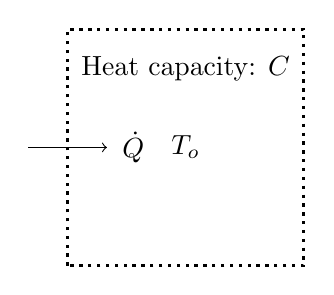
\begin{tikzpicture}
\draw[dotted,very thick]  (-1.5,-1.5) rectangle (1.5,1.5);
\draw (0,0) node {$T_{o}$};
\draw (0,1) node {Heat capacity: $C$};
\draw[->] (-2,0) -- ++(1,0) node[right=2pt] {$\dot{Q}$}; 
\end{tikzpicture} 
& 
%--------- Thermal Convection ''Heat Flow''
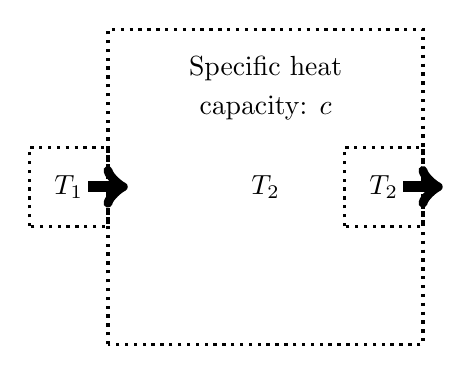
\begin{tikzpicture}
\draw[dotted,very thick]  (-2,-2) rectangle (2,2);
\draw[dotted,very thick]  (-3,-0.5) rectangle ++(1,1);
\draw[dotted,very thick]  (1,-0.5) rectangle ++(1,1);
\draw (0,1.5) node {Specific heat};
\draw (0,1.0) node {capacity: $c$};
\draw (0,0) node {$T_{2}$};
\draw (-2.5,0) node {$T_{1}$};
\draw (1.5,0) node {$T_{2}$};
\draw[->,line width=4pt] (-2.25,0) -- ++(.5,0);
\draw[->,line width=4pt] (1.75,0) -- ++(.5,0);
 \end{tikzpicture}  
 \\\hline

\rule[-8pt]{0pt}{0pt}\rule{0pt}{14pt}  
Component law & 		$T = \dot{Q}R$ & 
							$\dot{Q} = C \frac{dT_o}{dt}$ & 
							$\dot{Q} = \dot{m} c T$ \\\hline
							
\rule[-8pt]{0pt}{0pt}\rule{0pt}{14pt}							
Laplace Transform &	$T(s)=\dot{Q}(s)R$ & 
							$\dot{Q}(s)=CsT_o(s)$ & 
							$\dot{Q}(s)=\dot{m}cT(s)$ \\\hline

 							 
Impedance Component  &  
 %--------- Thermal resistance model
 \begin{tikzpicture}
\draw (5,0) node[inner sep=0,outer sep=0] (C) {\input{../DrawingElements/CircuitElements/resistor.tex}};
\draw (C) node[above=12pt] {$R$};
\draw[->] (C.0) ++(.1,0) -- node[pos=.5,below=2pt] {$\dot{Q}$} ++(.5,0);
\draw[<-] (C.180) ++(-.1,0) -- node[pos=.5,below=2pt] {$\dot{Q}$} ++(-.5,0);
\draw (C.0) node[draw,fill,inner sep=0pt,outer sep=0pt,circle] {$\rule{2pt}{0pt}$};
\draw (C.0) node[above=4pt] {$T_{2}$};
\draw (C.180) node[draw,fill,inner sep=0pt,outer sep=0pt,circle] {$\rule{2pt}{0pt}$};
\draw (C.180) node[above=4pt] {$T_{1}$};
%\draw (C) ++(0,-1) node {$\dot{Q}R = T_{1} - T_{2}$};
\draw (C) ++(0,-1) node {$T = T_{1} - T_{2}$};
\end{tikzpicture} 
& 
%--------- Thermal capacitor model
 \begin{tikzpicture} 
\draw (5,0) node[inner sep=0,outer sep=0,rotate=90] (C) {\input{../DrawingElements/CircuitElements/capacitor.tex}};
\draw (C) node[right=12pt] {$\frac{1}{Cs}$};
\draw[->] (C.0) ++(.3,0) -- node[pos=0,right=2pt] {$\dot{Q}$} ++(0,-.5);
\draw (C.0) node[draw,fill,inner sep=0pt,outer sep=0pt,circle] {$\rule{2pt}{0pt}$};
\draw (C.0) node[above=4pt] {$T_{o}$};
\draw (C.180) node[draw,fill,inner sep=0pt,outer sep=0pt,circle] {$\rule{2pt}{0pt}$};
\draw (C.180) node[below=4pt] {$T_{ref}=0$}; 
\end{tikzpicture} 
& 
 \begin{tikzpicture} 
\draw (7,0) node (C) {\input{../DrawingElements/CircuitElements/resistor.tex}};
\draw (5,0) node[isosceles triangle,draw,very thick,inner sep=2pt] (G) {$1$};
\draw (C) node[above=12pt] {$R=\frac{1}{c\dot{m}}$};
\draw[very thick] (G.180) ++(-.75,0) node[draw,fill,inner sep=0pt,outer sep=0pt,circle] (Gin) {$\rule{2pt}{0pt}$} -- (G.180);
\draw (Gin) node[above=4pt] {$T_{1}$};
\draw[<-] (Gin) ++(-.1,0) -- node[pos=-1.5,below left=2pt] {$\dot{Q}_{in}=0$} ++(-.5,0);
\draw[very thick] (G.0) ++(-0.1,0) --   ++(0.8,0) ;
\draw[very thick] (C.0) ++(-0.2,0) -- ++(.5,0) node (C_p) {} node[above=4pt]  {$T_{2}$};
\draw (C_p.0)++(-0.1,0) node[draw,fill,inner sep=0pt,outer sep=0pt,circle] {$\rule{2pt}{0pt}$};
\draw[->] (C_p.0) ++(.1,0) -- node[pos=-.5,below right=2pt] {$\dot{Q}$} ++(.5,0);
\draw (C) ++(0,-1) node {$T = T_{1} - T_{2}$};
\end{tikzpicture}

\end{tabular}
\end{center}
\end{frame}


%%%%%%%%%%%%%%%%%%%%%%%%%%%%%%%%%%%
\begin{frame}{DC Motor}
\begin{center}
\begin{tabular}{c|c}
   &   DC motor \\\hline
   
Component & 
\begin{tikzpicture}[scale=1.3,inner sep=0pt,outer sep=0pt,very thick]
\draw (0,0) node[fill=black] (a) {}; 
\draw (3.5,0) node[fill=black] (c) {};
\draw (0,-2) node[fill=black] (d) {};
\draw (2,-2) node[fill=black] (e) {};
\draw (3.5,-2) node[fill=black] (f) {};
 
\draw (1,0) node (R1) {\input{../DrawingElements/CircuitElements/resistor.tex}};
\draw (1,0) node[above=.2in] {$R_{a}$};
\draw (2.5,0) node (L1) {\input{../DrawingElements/CircuitElements/inductor.tex}};
\draw (2.5,0) node[above=.2in] {$L_{a}$};
\draw (3.5,-1) node (Rot) {\input{../DrawingElements/CircuitElements/rotor.tex}}; 
\draw[->] (4,-1) ++(0,.5)  node[above=2pt] {$\theta$}  .. controls  ++(-.15,-.3) and ++(-.15,.3) ..  ++(0,-1);
\draw[->] (4.25,-1) ++(0,.5) node[above=2pt] {$\tau_{m}$}  .. controls  ++(-.15,-.3) and ++(-.15,.3) ..  ++(0,-1);
\draw[->] (3.35,-.1) -- node[left=1pt] {$i_{a}$} ++(0,-.5); 
\draw (3.5,-1) node[left=.2in] {$\begin{matrix} + \\ v_{b} \\ -\end{matrix}$};
\draw (0,-1) node (V) {\input{../DrawingElements/CircuitElements/voltagesource.tex}};
\draw (0,-1) node[left=.2in]{$v_{a}$};
\draw (a) -- (R1);
\draw (R1) -- (L1);
\draw (L1) -| (Rot);
\draw (Rot) -- (f);
\draw (f) -- (d);
\draw (a) -- (V);
\draw (d) -- (V);


\end{tikzpicture}
 \\\hline
 
 						 
Component Law &  	
\pbox{10cm}
{$v_{b} = K_{e}\dot{\theta}$ \\ 
$\tau_{m} = K_{t} i_{a}$ \\ 
$v_a(t) = i_a(t)R + L\frac{di_a(t)}{dt} + v_b(t)$ }

\\\hline
 							 
Block Diagram  &  
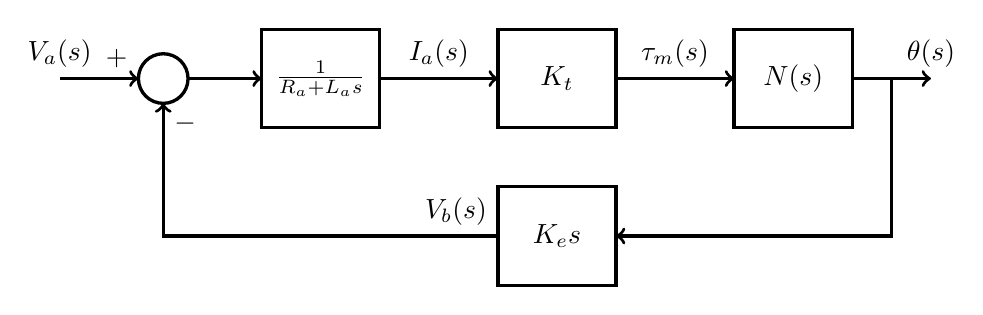
\begin{tikzpicture}[inner sep=0pt,outer sep=0pt,very thick,
sysblock/.style={draw,rectangle,inner sep=2pt,minimum width=1.5cm,minimum height=1.25cm,very thick}]
\draw (0,0) node[draw,circle] (sum) {$\rule{0pt}{18pt}$};
\draw (2,0) node[sysblock] (a) {$\frac{1}{R_{a} + L_{a}s}$};
\draw (5,0) node[sysblock] (b) {$K_{t}$};
\draw (8,0) node[sysblock] (c) {$N(s)$};
\draw (5,-2) node[sysblock] (d) {$K_{e}s$};
\draw[<-] (sum.180) node[above left=4pt] {$+$} -- ++(-1,0) node[above=4pt] {$V_{a}(s)$};
\draw[->] (sum.0) -- (a.180);
\draw[->] (a.0) -- node[pos=.5,above=4pt] {$I_{a}(s)$} (b.180);
\draw[->] (b.0) -- node[pos=.5,above=4pt] {$\tau_{m}(s)$} (c.180);
\draw[->] (c.0) -- ++(1,0) node[above=4pt] {$\theta(s)$};
\draw[->] (c.0) -- ++(.5,0) |- (d.0);
\draw[->] (d.180) node[above left=4pt] {$V_{b}(s)$} -| (sum.-90) node[below right=4pt] {$-$};
\end{tikzpicture}  
\end{tabular}
\end{center}
\end{frame}


%%%%%%%%%%%%%%%%%%%%%%%%%%%%%%%%%%%
\pagebreak
\begin{frame}{Hydraulic}
\begin{center}
\begin{tabular}{c|c}
   &   Hydraulic \\\hline

Component &    
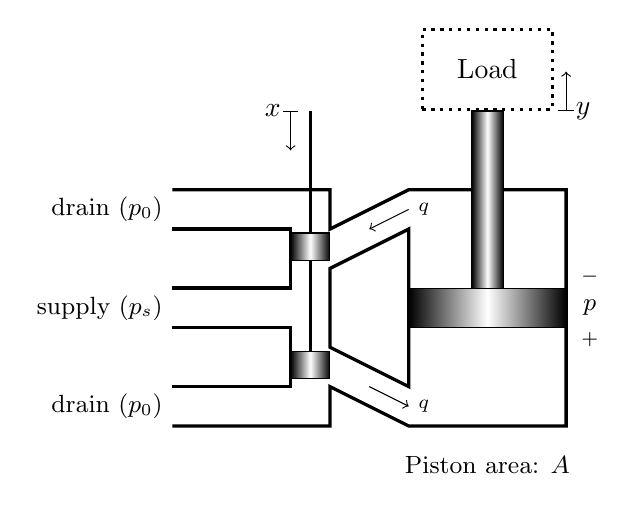
\begin{tikzpicture}
% tank
\draw[very thick] (0,0) -- ++(2,0) -- ++(0,-.5) -- ++(1,.5) -- ++(2,0) -- ++(0,-3) -- ++(-2,0) -- ++(-1,.5) -- ++(0,-.5) -- ++(-2,0);
\draw[very thick] (0,-.5) -- ++(1.5,0) -- ++(0,-.75) -- ++(-1.5,0);
\draw[very thick] (0,-1.75) -- ++(1.5,0) -- ++(0,-.75) -- ++(-1.5,0);
\draw[very thick] (2,-1) -- ++(1,.5) -- ++(0,-2) -- ++(-1,.5) -- cycle;
\draw (4,-3.5) node {\small Piston area: $A$};
\draw (0,-.25) node[left] {\small drain ($p_{0}$)};
\draw (0,-1.5) node[left] {\small supply ($p_{s}$)};
\draw (0,-2.75) node[left] {\small drain ($p_{0}$)};
\draw[->] (3,-.25) node[right] {\scriptsize$q$} -- ++(-.5,-.25);
\draw[->] (2.5,-2.5) -- ++(.5,-.25)  node[right] {\scriptsize$q$};
\draw (5.3,-1.9) node {\scriptsize $+$} ++(0,.4) node{\small $p$} ++(0,.4) node {\scriptsize$-$};

% valves
\draw[very thick,color=black] (1.75,-2.1) -- ++(0,3.1);
\draw[fill,left color=black,right color=black,middle color=white] (1.5,-.9) rectangle ++(.5,.35);
\draw[fill,left color=black,right color=black,middle color=white] (1.5,-2.4) rectangle ++(.5,.35);
\draw[|->] (1.5,1) node[left] {$x$} -- ++(0,-.5); 

% piston
\draw[fill,left color=black,right color=black,middle color=white] (4,-1.5) ++(-.2,0) rectangle ++(.4,2.5);
\draw[fill,left color=black,right color=black,middle color=white] (3,-1.75) rectangle ++(2,.5);
\draw[|->] (5,1) node[right] {$y$} -- ++(0,.5);

% load
\draw (4,1) node[draw,very thick,above,dotted,rectangle,minimum width=.65in,minimum height=.4in] {Load};
\end{tikzpicture}
\\\hline

\rule[-8pt]{0pt}{0pt}
Component Law &  
\pbox{10cm}
{$\delta q = k_x\delta x - k_p \delta p$ \\
$f = p A $ \\
$y = \frac{1}{A} \int q dt $ }

\\\hline

Block Diagram & 
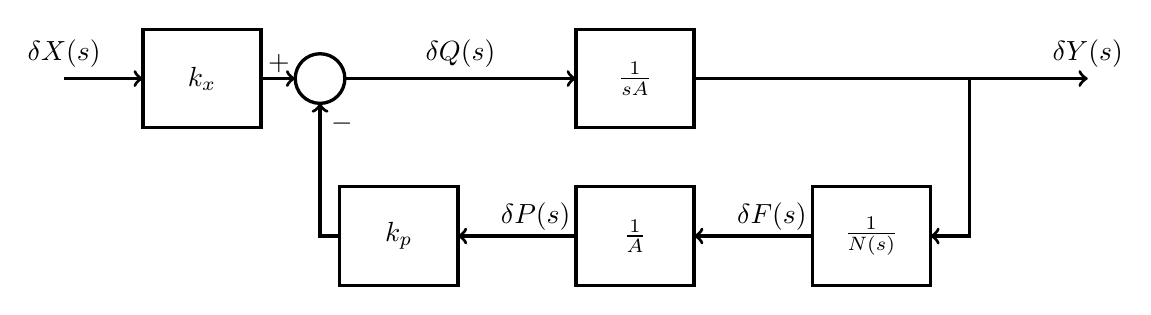
\begin{tikzpicture}[inner sep=0pt,outer sep=0pt,very thick,
sysblock/.style={draw,rectangle,inner sep=2pt,minimum width=1.5cm,minimum height=1.25cm,very thick}]
\draw (-1.5,0) node[sysblock] (d) {$k_{x}$};
\draw (0,0) node[draw,circle] (sum) {$\rule{0pt}{18pt}$};
\draw (4,0) node[sysblock] (a) {$\frac{1}{sA}$};
\draw (4,-2) node[sysblock] (b) {$\frac{1}{A}$};
\draw (7,-2) node[sysblock] (b1) {$\frac{1}{N(s)}$};
\draw (1,-2) node[sysblock] (c) {$k_{p}$};
\draw[<-] (d.180)  -- ++(-1,0) node[above=4pt] {$\delta X(s)$};
\draw[->] (d.0) -- (sum.180) node[above left=2pt] {$+$};
\draw[->] (sum.0) -- node[pos=.5,above=4pt] {$\delta Q(s)$} (a.180);
\draw[->] (a.0) -- ++(5,0) node[above=4pt] {$\delta Y(s)$};
\draw[->] (a.0) -- ++(3.5,0) |- (b1.0);
\draw[->] (b1.180) node[above left=2pt] {$\delta F(s)$} -- (b.0);
\draw[->] (b.180) node[above left=2pt] {$\delta P(s)$} -- (c.0);
\draw[->] (c.180)  -| (sum.-90) node[below right=4pt] {$-$};

\end{tikzpicture}





\end{tabular}
\end{center}
\end{frame}

\end{document}


};
\draw (k) node[above=6pt] {$\frac{1}{k}$};
\draw (1.5,-.5) node (b) {\documentclass[12pt]{article}
% \newcommand{\mainfolder}{/Users/coulston/Dropbox/EENG307Current}  	                    % @ Work PC
%\newcommand{\mainfolder}{C:/Users/Chris/Dropbox/Mycourses/EENG307Current}  	% @ Work Laptop
\newcommand{\mainfolder}{C:/Users/chris/Dropbox/Mycourses/EENG307Current}		% @ Home PC

% \newcommand{\mainfolder}{$HOME/Dropbox/EENG307Current}
\newcommand{\commonmaterial}{\mainfolder/CommonMaterial}
\input{\mainfolder/Headers/packageheader}
\input{\mainfolder/Headers/coursedefheader}

\usepackage{pbox}
%\usepackage{siunitx}
%\usepackage{draftwatermark}
%\SetWatermarkText{DRAFT}
%\SetWatermarkScale{1}

\setlength{\topmargin}{-.75in}
\setlength{\textheight}{9.25in}
\setlength{\oddsidemargin}{-0.25in}
\setlength{\evensidemargin}{-0.25in}
\setlength{\textwidth}{7in}




\begin{document}



%%%%%%%%%%%%%%%%%%%%%%%%%%%%%%%%%%%
\begin{frame}{Electrical Impedance}%
\begin{center}%
\mode<article>{

\begin{tabular}{c|ccc}
 & resistor & capacitor & inductor  \\\hline
 Component & \input{./figures/resistor.tex} & \input{./figures/capacitor.tex} & \input{./figures/inductor.tex}\\\hline
\rule[-8pt]{0pt}{0pt}\rule{0pt}{14pt} 
Component law & $v_1-v_2=iR$ & $i = C\frac{d(v_1-v_2)}{dt}$ & $v_1-v_2=L\frac{di}{dt}$  \\\hline
\rule[-8pt]{0pt}{0pt}\rule{0pt}{14pt} 
Laplace Transform & $V(s)= I(s)R$ & $V(s) = \frac{1}{Cs}I(s)$ & $V(s) = LsI(s)$ \\\hline
Impedance Component & \input{./figures/resistorimpedance.tex} & \input{./figures/capacitorimpedance.tex} & \input{./figures/inductorimpedance.tex}

\end{tabular}}
\end{center}
\end{frame}


%%%%%%%%%%%%%%%%%%%%%%%%%%%%%%%%%%%
\begin{frame}{Fluid Impedance}
\graphicspath{}
\begin{center}
\mode<article>{

\begin{tabular}{c|cc}
 & valve & tank \\\hline
%Component &\begin{tikzpicture}
\draw (.75,0) node (valve) {\input{\mainfolder/DrawingElements/FluidElements/valve.tex}};
\draw (.75,0) node[above=9pt] {$R$};
\draw (-.2,.25) node[above] {$p_{1}$};
\draw[<-] (valve.180) --  ++(-.5,0) node[left] {$q$};
\draw[->] (valve.0) -- ++(.5,0)  node[right] {$q$};
\draw (1.7,.25) node[above] {$p_{2}$};
\draw (.75,1.5) node {$p = p_{1}-p_{2}$};
\end{tikzpicture} &  \input{./figures/figurestank2.tex} \\\hline
Component &\begin{tikzpicture}
\draw (.75,0) node (valve) {\input{\mainfolder/DrawingElements/FluidElements/valve.tex}};
\draw (.75,0) node[above=9pt] {$R$};
\draw (-.2,.25) node[above] {$p_{1}$};
\draw[<-] (valve.180) --  ++(-.5,0) node[left] {$q$};
\draw[->] (valve.0) -- ++(.5,0)  node[right] {$q$};
\draw (1.7,.25) node[above] {$p_{2}$};
\draw (.75,1.5) node {$p = p_{1}-p_{2}$};
\end{tikzpicture} &  \input{./figures/tank.tex} \\\hline
\rule[-8pt]{0pt}{0pt}\rule{0pt}{14pt} Component law & $p=Rq$ & $\frac{A}{\rho g}\frac{dp}{dt} = q_{1} - q_{2}$ \\\hline
\rule[-8pt]{0pt}{0pt}\rule{0pt}{14pt} Laplace Transform & $P(s)= RQ(s)$ & $\frac{A}{\rho g}sP(s) = Q_{1}(s)-Q_{2}(s)$ \\\hline
 Impedance Component & \input{./figures/valveanalogycopy.tex} & \input{./figures/tankanalogycopy.tex}
 \end{tabular}}
 
\mode<presentation>{\resizebox{11cm}{!}{

\begin{tabular}{c|cc}
 & valve & tank \\\hline
Component &\begin{tikzpicture}
\draw (.75,0) node (valve) {\input{\mainfolder/DrawingElements/FluidElements/valve.tex}};
\draw (.75,0) node[above=9pt] {$R$};
\draw (-.2,.25) node[above] {$p_{1}$};
\draw[<-] (valve.180) --  ++(-.5,0) node[left] {$q$};
\draw[->] (valve.0) -- ++(.5,0)  node[right] {$q$};
\draw (1.7,.25) node[above] {$p_{2}$};
\draw (.75,1.5) node {$p = p_{1}-p_{2}$};
\end{tikzpicture} & \input{./figures/tank2.tex} \\\hline
\rule[-8pt]{0pt}{0pt}\rule{0pt}{14pt} Component law & $p=Rq$ & $\frac{A}{\rho g}\frac{dp}{dt} = q_{1} - q_{2}$ \\\hline
\rule[-8pt]{0pt}{0pt}\rule{0pt}{14pt} Laplace Transform & $P(s)= RQ(s)$ & $\frac{A}{\rho g}sP(s) = Q_{1}(s)-Q_{2}(s)$ \\\hline
 Impedance Component & \input{./figures/valveanalogycopy.tex} & \input{./figures/tankanalogycopy.tex}
 \end{tabular}}}
\end{center}
\end{frame}

\pagebreak

%%%%%%%%%%%%%%%%%%%%%%%%%%%%%%%%%%%
\begin{frame}{Mechanical Impedance}%
\begin{center}%
\mode<article>{\begin{tabular}{c|ccc}
 & mass & spring & damper \\\hline
 Component & \begin{tikzpicture}
%  \draw(-1,2.5) node (text) {\textsf{fixed point}};
%   \draw[->] (text.180) -- ++(-.7,0);
   \draw[inner sep=0pt,outer sep=0pt,very thick] (-3,1) node (gnd1) {\input{\mainfolder/DrawingElements/MechanicalElements/ground.tex}};
   \draw[->|,dotted] (-3,1.75) -- node[pos=.5,above] {$x_{f}$} ++(3.6,0); 
    \draw[very thick] (0,0) rectangle (1.2,1);
    \draw (.6,.5) node {$m$};
    \draw[->,thick] (1.2,.5) -- ++(.5,0) node[right] {$f$};
    \draw[|->,thick] (.6,1.2) node[above=2pt] {$x$} -- ++(.5,0);  
\end{tikzpicture}
 & \begin{tikzpicture}
\draw (.75,0) node[inner sep=0,outer sep=0] (K1) {\input{\mainfolder/DrawingElements/MechanicalElements/spring.tex}};
\draw (K1)  node[above=6pt] {$k$};
\draw[very thick] (K1.180) -- ++(-.2,0);
\draw[very thick] (K1.0) -- ++(0.2,0);
\draw[<-,thick] (K1.0) ++(.2,0) -- ++(.5,0) node[right] {$f$};
\draw[<-,thick] (K1.180) ++(-.2,0) -- ++(-.5,0) node[left] {$f$};
\draw[|->,thick] (K1.180) ++(-.2,.4) node[above=2pt] {$x_{1}$} -- ++(.5,0);  
\draw[|->,thick] (K1.0) ++(.2,.4) node[above=2pt] {$x_{2}$} -- ++(.5,0);  
\draw<2-> (K1) ++(0,-.6) node {$f=k(x_{1}-x_{2})$};
\end{tikzpicture}
 & \begin{tikzpicture}
\draw[very thick] (-.2,0) -- (0,0);
\draw (.75,0) node {\input{\mainfolder/DrawingElements/MechanicalElements/damper.tex}};
\draw (.75,0) node[above=9pt] {$b$};
\draw[very thick] (1.5,0) -- ++(.2,0);
    \draw[<-,thick] (1.5,0) ++(.2,0) -- ++(.5,0) node[right] {$f$};
    \draw[<-,thick] (-.2,0) -- ++(-.5,0) node[left] {$f$};
    \draw[|->,thick] (-.2,.4) node[above=2pt] {$x_{1}$} -- ++(.5,0);  
    \draw[|->,thick] (1.7,.4) node[above=2pt] {$x_{2}$} -- ++(.5,0);  
    \draw (.6,-.6) node {$x=x_{1}-x_{2}$};
  %  \draw (.6,-1.2) node {$f=b\dot{x}$};
\end{tikzpicture}\\\hline
\rule[-8pt]{0pt}{0pt}\rule{0pt}{14pt} 
Component law & $f = m\ddot{x}$ & $f = kx$ & $f=b\dot{x}$  \\\hline
\rule[-8pt]{0pt}{0pt}\rule{0pt}{14pt} Laplace Transform & $X(s)= \frac{1}{ms^{2}}F(s)$ & $X(s) = \frac{1}{k}F(s)$ & $X(s) = \frac{1}{bs}F(s)$ \\\hline
\begin{minipage}[b]{1.5in}\begin{center}Impedance Component \\
(positive $f$ direction agrees with positive $x$ direction)\end{center}
\end{minipage}
& \input{figures/massimpedance.tex} & \input{figures/springimpedance.tex} & \input{figures/damperimpedance.tex}
 \end{tabular}}
\mode<presentation>{\resizebox{10cm}{!}{\begin{tabular}{c|ccc}
 & mass & spring & damper \\\hline
 Component & \begin{tikzpicture}
%  \draw(-1,2.5) node (text) {\textsf{fixed point}};
%   \draw[->] (text.180) -- ++(-.7,0);
   \draw[inner sep=0pt,outer sep=0pt,very thick] (-3,1) node (gnd1) {\input{\mainfolder/DrawingElements/MechanicalElements/ground.tex}};
   \draw[->|,dotted] (-3,1.75) -- node[pos=.5,above] {$x_{f}$} ++(3.6,0); 
    \draw[very thick] (0,0) rectangle (1.2,1);
    \draw (.6,.5) node {$m$};
    \draw[->,thick] (1.2,.5) -- ++(.5,0) node[right] {$f$};
    \draw[|->,thick] (.6,1.2) node[above=2pt] {$x$} -- ++(.5,0);  
\end{tikzpicture}
& \begin{tikzpicture}
\draw (.75,0) node[inner sep=0,outer sep=0] (K1) {\input{\mainfolder/DrawingElements/MechanicalElements/spring.tex}};
\draw (K1)  node[above=6pt] {$k$};
\draw[very thick] (K1.180) -- ++(-.2,0);
\draw[very thick] (K1.0) -- ++(0.2,0);
\draw[<-,thick] (K1.0) ++(.2,0) -- ++(.5,0) node[right] {$f$};
\draw[<-,thick] (K1.180) ++(-.2,0) -- ++(-.5,0) node[left] {$f$};
\draw[|->,thick] (K1.180) ++(-.2,.4) node[above=2pt] {$x_{1}$} -- ++(.5,0);  
\draw[|->,thick] (K1.0) ++(.2,.4) node[above=2pt] {$x_{2}$} -- ++(.5,0);  
\draw<2-> (K1) ++(0,-.6) node {$f=k(x_{1}-x_{2})$};
\end{tikzpicture}
 & \begin{tikzpicture}
\draw[very thick] (-.2,0) -- (0,0);
\draw (.75,0) node {\input{\mainfolder/DrawingElements/MechanicalElements/damper.tex}};
\draw (.75,0) node[above=9pt] {$b$};
\draw[very thick] (1.5,0) -- ++(.2,0);
    \draw[<-,thick] (1.5,0) ++(.2,0) -- ++(.5,0) node[right] {$f$};
    \draw[<-,thick] (-.2,0) -- ++(-.5,0) node[left] {$f$};
    \draw[|->,thick] (-.2,.4) node[above=2pt] {$x_{1}$} -- ++(.5,0);  
    \draw[|->,thick] (1.7,.4) node[above=2pt] {$x_{2}$} -- ++(.5,0);  
    \draw (.6,-.6) node {$x=x_{1}-x_{2}$};
  %  \draw (.6,-1.2) node {$f=b\dot{x}$};
\end{tikzpicture}\\\hline
\rule{0pt}{14pt} Component law & $M\ddot{x}=f$ & $f = kx$ & $f=b\dot{x}$  \\\hline
\rule[-8pt]{0pt}{0pt}\rule{0pt}{14pt} Laplace Transform & $X(s)= \frac{1}{Ms^{2}}F(s)$ & $X(s) = \frac{1}{k}F(s)$ & $X(s) = \frac{1}{bs}F(s)$ \\\hline
\begin{minipage}[b]{1.5in}\begin{center}Impedance Component \\
(positive $f$ direction agrees with positive $x$ direction)\end{center}
\end{minipage}
& \input{./figures/massimpedance.tex} & \input{./figures/springimpedance.tex} & \input{./figures/damperimpedance.tex}
 \end{tabular}}}
\end{center}
\end{frame}


%%%%%%%%%%%%%%%%%%%%%%%%%%%%%%%%%%%
\begin{frame}{Rotational Impedance}
\begin{center}
\mode<article>{\begin{tabular}{c|ccc}
 & mass & spring & damper \\\hline
 Component & \begin{minipage}[b]{.75in}\begin{tikzpicture}
    \draw[very thick] (.5,0) node[cylinder,draw,shape aspect=.55,minimum width=1cm,minimum height=1.5cm] (J) {$J$};
    \draw[->] (-.2,.5) node[above] {$\theta$}  .. controls  ++(-.15,-.3) and ++(-.15,.3) ..  ++(0,-1);
    \draw[->] (1.4,-.5) node[below] {$\tau$}  .. controls  ++(.15,.3) and ++(.15,-.3) ..  ++(0,1);
    \draw (.5,-1) node {$J\ddot{\theta}=\tau$};
\end{tikzpicture}\\\vspace{.1in}\end{minipage} & \begin{tikzpicture}
\draw[very thick] (-.2,0) -- (0,0);
\draw (.75,0) node {\input{\mainfolder/DrawingElements/MechanicalElements/spring.tex}};
\draw[very  thick] (1.5,0) -- ++(.2,0);
\draw (.75,0) node[above=9pt] {$k$};
\draw[->] (-.2,.5) node[above] {$\theta_{1}$}  .. controls  ++(-.15,-.3) and ++(-.15,.3) ..  ++(0,-1);
\draw[->] (-.5,.5) node[above] {$\tau$}  .. controls  ++(-.15,-.3) and ++(-.15,.3) ..  ++(0,-1);
\draw[->] (1.5,.5) node[above] {$\theta_{2}$}  .. controls  ++(-.15,-.3) and ++(-.15,.3) ..  ++(0,-1);
\draw[->] (1.9,.5) node[above] {$\tau$}  .. controls  ++(.15,-.3) and ++(.15,.3) ..  ++(0,-1);
\draw (.5,-1) node {$\theta=\theta_{1} - \theta_{2}$};
\end{tikzpicture} & \begin{tikzpicture}
\draw[very thick] (-.2,0) -- (0,0);
\draw (.75,0) node {\input{\mainfolder/DrawingElements/MechanicalElements/damper.tex}};
\draw[very  thick] (1.5,0) -- ++(.2,0);
\draw (.75,0) node[above=9pt] {$b$};
\draw[->] (-.2,.5) node[above] {$\theta_{1}$}  .. controls  ++(-.15,-.3) and ++(-.15,.3) ..  ++(0,-1);
\draw[->] (-.5,.5) node[above] {$\tau$}  .. controls  ++(-.15,-.3) and ++(-.15,.3) ..  ++(0,-1);
\draw[->] (1.5,.5) node[above] {$\theta_{2}$}  .. controls  ++(-.15,-.3) and ++(-.15,.3) ..  ++(0,-1);
\draw[->] (1.9,.5) node[above] {$\tau$}  .. controls  ++(.15,-.3) and ++(.15,.3) ..  ++(0,-1);
\draw (.5,-1) node {$\dot{\theta}=\dot{\theta}_{1} - \dot{\theta}_{2}$};
\end{tikzpicture}\\\hline
 \rule[-8pt]{0pt}{0pt}\rule{0pt}{12pt} 
 Component Law & $\tau = J\ddot{\theta}$ & $\tau = k\theta$ & $\tau = b\dot{\theta}$ \\\hline
\rule[-8pt]{0pt}{0pt}\rule{0pt}{14pt} Laplace Transform & $\theta(s)= \frac{1}{Js^{2}}\tau(s)$ & $\theta(s) = \frac{1}{k}\tau(s)$ & $\theta(s) = \frac{1}{bs}\tau(s)$ \\\hline
\begin{minipage}[b]{1.5in}\begin{center}Impedance Component
\end{center}
\end{minipage}
& \begin{tikzpicture}
\draw (0,0) node (R) {\begin{tikzpicture}
\draw (0,0) node[circle,fill,inner sep=1pt,] {} node[above] {$\theta$};
\draw[very thick] (0,0)  -- ++(0,-.37);
\draw[very thick] (0,-1) node[rectangle,draw,minimum width=.1in,minimum height=.5in] {};
\draw[very thick] (0,-1.65) -- ++(0,-.37);
\draw[very thick] (0,-2) node{\input{\mainfolder/DrawingElements/CircuitElements/elground.tex}};
\end{tikzpicture}
};

\draw (R) node[right=6pt] {$\frac{1}{Js^{2}}$};
%\draw (6.1,.75) node[above] {$+$};
\draw (1,0) node[right] {$\begin{matrix} + \\ \\ \theta(s)\\  \\ - \end{matrix}$};
%\draw (7.9,.75) node[above] {$-$};
\draw[->] (-.3,.5) -- node[pos=.5,left] {$\tau(s)$} ++(0,-1);  

\end{tikzpicture} & \begin{tikzpicture}
\draw (7,.2) node (R) {\begin{tikzpicture}
\draw (0,0) node[circle,fill,inner sep=1pt,] {} node[above] {$\theta_{1}$};
\draw[very thick] (0,0) -- ++(.37,0);
\draw[very thick] (1,0) node[rectangle,draw,minimum width=.5in,minimum height=.1in] {};
\draw[very thick] (1.65,0) -- ++(.37,0);
\draw (2.02,0) node[circle,fill,inner sep=1pt,] {} node[above] {$\theta_{2}$};
\end{tikzpicture}
};
\draw (R) node[above=1pt] {$\frac{1}{k}$};
%\draw (6.1,.75) node[above] {$+$};
%\draw (7,.75) node[above] {$X(s)$};
%\draw (7.9,.75) node[above] {$-$};
\draw[->] (6.5,-.3) -- node[pos=.5,below] {$\tau(s)$} ++(1,0);  
\draw (7,-1.5) node[above] {$\begin{matrix} + & \theta(s) & - \end{matrix}$};

\end{tikzpicture} & \input{./figures/rotdamperimpedance.tex}
 \end{tabular}}
\mode<presentation>{\resizebox{10cm}{!}{\begin{tabular}{c|ccc}
 & mass & spring & damper \\\hline
 Component & \begin{tikzpicture}
    \draw[very thick] (.5,0) node[cylinder,draw,shape aspect=.55,minimum width=1cm,minimum height=1.5cm] (J) {$J$};
    \draw[->] (-.2,.5) node[above] {$\theta$}  .. controls  ++(-.15,-.3) and ++(-.15,.3) ..  ++(0,-1);
    \draw[->] (1.4,-.5) node[below] {$\tau$}  .. controls  ++(.15,.3) and ++(.15,-.3) ..  ++(0,1);
    \draw (.5,-1) node {$J\ddot{\theta}=\tau$};
\end{tikzpicture} & \begin{tikzpicture}
\draw[very thick] (-.2,0) -- (0,0);
\draw (.75,0) node {\input{\mainfolder/DrawingElements/MechanicalElements/spring.tex}};
\draw[very  thick] (1.5,0) -- ++(.2,0);
\draw (.75,0) node[above=9pt] {$k$};
\draw[->] (-.2,.5) node[above] {$\theta_{1}$}  .. controls  ++(-.15,-.3) and ++(-.15,.3) ..  ++(0,-1);
\draw[->] (-.5,.5) node[above] {$\tau$}  .. controls  ++(-.15,-.3) and ++(-.15,.3) ..  ++(0,-1);
\draw[->] (1.5,.5) node[above] {$\theta_{2}$}  .. controls  ++(-.15,-.3) and ++(-.15,.3) ..  ++(0,-1);
\draw[->] (1.9,.5) node[above] {$\tau$}  .. controls  ++(.15,-.3) and ++(.15,.3) ..  ++(0,-1);
\draw (.5,-1) node {$\theta=\theta_{1} - \theta_{2}$};
\end{tikzpicture} & \begin{tikzpicture}
\draw[very thick] (-.2,0) -- (0,0);
\draw (.75,0) node {\input{\mainfolder/DrawingElements/MechanicalElements/damper.tex}};
\draw[very  thick] (1.5,0) -- ++(.2,0);
\draw (.75,0) node[above=9pt] {$b$};
\draw[->] (-.2,.5) node[above] {$\theta_{1}$}  .. controls  ++(-.15,-.3) and ++(-.15,.3) ..  ++(0,-1);
\draw[->] (-.5,.5) node[above] {$\tau$}  .. controls  ++(-.15,-.3) and ++(-.15,.3) ..  ++(0,-1);
\draw[->] (1.5,.5) node[above] {$\theta_{2}$}  .. controls  ++(-.15,-.3) and ++(-.15,.3) ..  ++(0,-1);
\draw[->] (1.9,.5) node[above] {$\tau$}  .. controls  ++(.15,-.3) and ++(.15,.3) ..  ++(0,-1);
\draw (.5,-1) node {$\dot{\theta}=\dot{\theta}_{1} - \dot{\theta}_{2}$};
\end{tikzpicture}\\\hline
\rule[-8pt]{0pt}{0pt}\rule{0pt}{14pt} Laplace Transform & $\theta(s)= \frac{1}{Js^{2}}\tau(s)$ & $\theta(s) = \frac{1}{k}\tau(s)$ & $\theta(s) = \frac{1}{bs}\tau(s)$ \\\hline
\begin{minipage}[b]{1.5in}\begin{center}Impedance Component 
\end{center}
\end{minipage}
& \begin{tikzpicture}
\draw (0,0) node (R) {\begin{tikzpicture}
\draw (0,0) node[circle,fill,inner sep=1pt,] {} node[above] {$\theta$};
\draw[very thick] (0,0)  -- ++(0,-.37);
\draw[very thick] (0,-1) node[rectangle,draw,minimum width=.1in,minimum height=.5in] {};
\draw[very thick] (0,-1.65) -- ++(0,-.37);
\draw[very thick] (0,-2) node{\input{\mainfolder/DrawingElements/CircuitElements/elground.tex}};
\end{tikzpicture}
};

\draw (R) node[right=6pt] {$\frac{1}{Js^{2}}$};
%\draw (6.1,.75) node[above] {$+$};
\draw (1,0) node[right] {$\begin{matrix} + \\ \\ \theta(s)\\  \\ - \end{matrix}$};
%\draw (7.9,.75) node[above] {$-$};
\draw[->] (-.3,.5) -- node[pos=.5,left] {$\tau(s)$} ++(0,-1);  

\end{tikzpicture} & \begin{tikzpicture}
\draw (7,.2) node (R) {\begin{tikzpicture}
\draw (0,0) node[circle,fill,inner sep=1pt,] {} node[above] {$\theta_{1}$};
\draw[very thick] (0,0) -- ++(.37,0);
\draw[very thick] (1,0) node[rectangle,draw,minimum width=.5in,minimum height=.1in] {};
\draw[very thick] (1.65,0) -- ++(.37,0);
\draw (2.02,0) node[circle,fill,inner sep=1pt,] {} node[above] {$\theta_{2}$};
\end{tikzpicture}
};
\draw (R) node[above=1pt] {$\frac{1}{k}$};
%\draw (6.1,.75) node[above] {$+$};
%\draw (7,.75) node[above] {$X(s)$};
%\draw (7.9,.75) node[above] {$-$};
\draw[->] (6.5,-.3) -- node[pos=.5,below] {$\tau(s)$} ++(1,0);  
\draw (7,-1.5) node[above] {$\begin{matrix} + & \theta(s) & - \end{matrix}$};

\end{tikzpicture} & \input{./figures/rotdamperimpedance.tex}
 \end{tabular}}}
\end{center}
\end{frame}


\pagebreak

%%%%%%%%%%%%%%%%%%%%%%%%%%%%%%%%%%%
\begin{frame}{Thermal Impedance}
\begin{center}
\begin{tabular}{c|ccc}
 & Resistance & Capacitance & Convection \\\hline
 
 
Component & 
%-------- Thermal Resistance :''Brick wall''
\begin{tikzpicture}
\draw[pattern=bricks]  (0,-2) -- ++(0,4) -- ++(.25,0) -- ++(0,-4)  -- cycle;
\draw (-1,1) node {$T_{1}$};
\draw (1,1) node {$T_{2}$};
\draw[->] (-.5,0) -- ++(1,0) node[right=2pt] {$\dot{Q}$}; 
\end{tikzpicture}
 & 
 %--------- Thermal Capacitance ''Heat Chamber''
\begin{tikzpicture}
\draw[dotted,very thick]  (-1.5,-1.5) rectangle (1.5,1.5);
\draw (0,0) node {$T_{o}$};
\draw (0,1) node {Heat capacity: $C$};
\draw[->] (-2,0) -- ++(1,0) node[right=2pt] {$\dot{Q}$}; 
\end{tikzpicture} 
& 
%--------- Thermal Convection ''Heat Flow''
\begin{tikzpicture}
\draw[dotted,very thick]  (-2,-2) rectangle (2,2);
\draw[dotted,very thick]  (-3,-0.5) rectangle ++(1,1);
\draw[dotted,very thick]  (1,-0.5) rectangle ++(1,1);
\draw (0,1.5) node {Specific heat};
\draw (0,1.0) node {capacity: $c$};
\draw (0,0) node {$T_{2}$};
\draw (-2.5,0) node {$T_{1}$};
\draw (1.5,0) node {$T_{2}$};
\draw[->,line width=4pt] (-2.25,0) -- ++(.5,0);
\draw[->,line width=4pt] (1.75,0) -- ++(.5,0);
 \end{tikzpicture}  
 \\\hline

\rule[-8pt]{0pt}{0pt}\rule{0pt}{14pt}  
Component law & 		$T = \dot{Q}R$ & 
							$\dot{Q} = C \frac{dT_o}{dt}$ & 
							$\dot{Q} = \dot{m} c T$ \\\hline
							
\rule[-8pt]{0pt}{0pt}\rule{0pt}{14pt}							
Laplace Transform &	$T(s)=\dot{Q}(s)R$ & 
							$\dot{Q}(s)=CsT_o(s)$ & 
							$\dot{Q}(s)=\dot{m}cT(s)$ \\\hline

 							 
Impedance Component  &  
 %--------- Thermal resistance model
 \begin{tikzpicture}
\draw (5,0) node[inner sep=0,outer sep=0] (C) {\input{../DrawingElements/CircuitElements/resistor.tex}};
\draw (C) node[above=12pt] {$R$};
\draw[->] (C.0) ++(.1,0) -- node[pos=.5,below=2pt] {$\dot{Q}$} ++(.5,0);
\draw[<-] (C.180) ++(-.1,0) -- node[pos=.5,below=2pt] {$\dot{Q}$} ++(-.5,0);
\draw (C.0) node[draw,fill,inner sep=0pt,outer sep=0pt,circle] {$\rule{2pt}{0pt}$};
\draw (C.0) node[above=4pt] {$T_{2}$};
\draw (C.180) node[draw,fill,inner sep=0pt,outer sep=0pt,circle] {$\rule{2pt}{0pt}$};
\draw (C.180) node[above=4pt] {$T_{1}$};
%\draw (C) ++(0,-1) node {$\dot{Q}R = T_{1} - T_{2}$};
\draw (C) ++(0,-1) node {$T = T_{1} - T_{2}$};
\end{tikzpicture} 
& 
%--------- Thermal capacitor model
 \begin{tikzpicture} 
\draw (5,0) node[inner sep=0,outer sep=0,rotate=90] (C) {\input{../DrawingElements/CircuitElements/capacitor.tex}};
\draw (C) node[right=12pt] {$\frac{1}{Cs}$};
\draw[->] (C.0) ++(.3,0) -- node[pos=0,right=2pt] {$\dot{Q}$} ++(0,-.5);
\draw (C.0) node[draw,fill,inner sep=0pt,outer sep=0pt,circle] {$\rule{2pt}{0pt}$};
\draw (C.0) node[above=4pt] {$T_{o}$};
\draw (C.180) node[draw,fill,inner sep=0pt,outer sep=0pt,circle] {$\rule{2pt}{0pt}$};
\draw (C.180) node[below=4pt] {$T_{ref}=0$}; 
\end{tikzpicture} 
& 
 \begin{tikzpicture} 
\draw (7,0) node (C) {\input{../DrawingElements/CircuitElements/resistor.tex}};
\draw (5,0) node[isosceles triangle,draw,very thick,inner sep=2pt] (G) {$1$};
\draw (C) node[above=12pt] {$R=\frac{1}{c\dot{m}}$};
\draw[very thick] (G.180) ++(-.75,0) node[draw,fill,inner sep=0pt,outer sep=0pt,circle] (Gin) {$\rule{2pt}{0pt}$} -- (G.180);
\draw (Gin) node[above=4pt] {$T_{1}$};
\draw[<-] (Gin) ++(-.1,0) -- node[pos=-1.5,below left=2pt] {$\dot{Q}_{in}=0$} ++(-.5,0);
\draw[very thick] (G.0) ++(-0.1,0) --   ++(0.8,0) ;
\draw[very thick] (C.0) ++(-0.2,0) -- ++(.5,0) node (C_p) {} node[above=4pt]  {$T_{2}$};
\draw (C_p.0)++(-0.1,0) node[draw,fill,inner sep=0pt,outer sep=0pt,circle] {$\rule{2pt}{0pt}$};
\draw[->] (C_p.0) ++(.1,0) -- node[pos=-.5,below right=2pt] {$\dot{Q}$} ++(.5,0);
\draw (C) ++(0,-1) node {$T = T_{1} - T_{2}$};
\end{tikzpicture}

\end{tabular}
\end{center}
\end{frame}


%%%%%%%%%%%%%%%%%%%%%%%%%%%%%%%%%%%
\begin{frame}{DC Motor}
\begin{center}
\begin{tabular}{c|c}
   &   DC motor \\\hline
   
Component & 
\begin{tikzpicture}[scale=1.3,inner sep=0pt,outer sep=0pt,very thick]
\draw (0,0) node[fill=black] (a) {}; 
\draw (3.5,0) node[fill=black] (c) {};
\draw (0,-2) node[fill=black] (d) {};
\draw (2,-2) node[fill=black] (e) {};
\draw (3.5,-2) node[fill=black] (f) {};
 
\draw (1,0) node (R1) {\input{../DrawingElements/CircuitElements/resistor.tex}};
\draw (1,0) node[above=.2in] {$R_{a}$};
\draw (2.5,0) node (L1) {\input{../DrawingElements/CircuitElements/inductor.tex}};
\draw (2.5,0) node[above=.2in] {$L_{a}$};
\draw (3.5,-1) node (Rot) {\input{../DrawingElements/CircuitElements/rotor.tex}}; 
\draw[->] (4,-1) ++(0,.5)  node[above=2pt] {$\theta$}  .. controls  ++(-.15,-.3) and ++(-.15,.3) ..  ++(0,-1);
\draw[->] (4.25,-1) ++(0,.5) node[above=2pt] {$\tau_{m}$}  .. controls  ++(-.15,-.3) and ++(-.15,.3) ..  ++(0,-1);
\draw[->] (3.35,-.1) -- node[left=1pt] {$i_{a}$} ++(0,-.5); 
\draw (3.5,-1) node[left=.2in] {$\begin{matrix} + \\ v_{b} \\ -\end{matrix}$};
\draw (0,-1) node (V) {\input{../DrawingElements/CircuitElements/voltagesource.tex}};
\draw (0,-1) node[left=.2in]{$v_{a}$};
\draw (a) -- (R1);
\draw (R1) -- (L1);
\draw (L1) -| (Rot);
\draw (Rot) -- (f);
\draw (f) -- (d);
\draw (a) -- (V);
\draw (d) -- (V);


\end{tikzpicture}
 \\\hline
 
 						 
Component Law &  	
\pbox{10cm}
{$v_{b} = K_{e}\dot{\theta}$ \\ 
$\tau_{m} = K_{t} i_{a}$ \\ 
$v_a(t) = i_a(t)R + L\frac{di_a(t)}{dt} + v_b(t)$ }

\\\hline
 							 
Block Diagram  &  
\begin{tikzpicture}[inner sep=0pt,outer sep=0pt,very thick,
sysblock/.style={draw,rectangle,inner sep=2pt,minimum width=1.5cm,minimum height=1.25cm,very thick}]
\draw (0,0) node[draw,circle] (sum) {$\rule{0pt}{18pt}$};
\draw (2,0) node[sysblock] (a) {$\frac{1}{R_{a} + L_{a}s}$};
\draw (5,0) node[sysblock] (b) {$K_{t}$};
\draw (8,0) node[sysblock] (c) {$N(s)$};
\draw (5,-2) node[sysblock] (d) {$K_{e}s$};
\draw[<-] (sum.180) node[above left=4pt] {$+$} -- ++(-1,0) node[above=4pt] {$V_{a}(s)$};
\draw[->] (sum.0) -- (a.180);
\draw[->] (a.0) -- node[pos=.5,above=4pt] {$I_{a}(s)$} (b.180);
\draw[->] (b.0) -- node[pos=.5,above=4pt] {$\tau_{m}(s)$} (c.180);
\draw[->] (c.0) -- ++(1,0) node[above=4pt] {$\theta(s)$};
\draw[->] (c.0) -- ++(.5,0) |- (d.0);
\draw[->] (d.180) node[above left=4pt] {$V_{b}(s)$} -| (sum.-90) node[below right=4pt] {$-$};
\end{tikzpicture}  
\end{tabular}
\end{center}
\end{frame}


%%%%%%%%%%%%%%%%%%%%%%%%%%%%%%%%%%%
\pagebreak
\begin{frame}{Hydraulic}
\begin{center}
\begin{tabular}{c|c}
   &   Hydraulic \\\hline

Component &    
\begin{tikzpicture}
% tank
\draw[very thick] (0,0) -- ++(2,0) -- ++(0,-.5) -- ++(1,.5) -- ++(2,0) -- ++(0,-3) -- ++(-2,0) -- ++(-1,.5) -- ++(0,-.5) -- ++(-2,0);
\draw[very thick] (0,-.5) -- ++(1.5,0) -- ++(0,-.75) -- ++(-1.5,0);
\draw[very thick] (0,-1.75) -- ++(1.5,0) -- ++(0,-.75) -- ++(-1.5,0);
\draw[very thick] (2,-1) -- ++(1,.5) -- ++(0,-2) -- ++(-1,.5) -- cycle;
\draw (4,-3.5) node {\small Piston area: $A$};
\draw (0,-.25) node[left] {\small drain ($p_{0}$)};
\draw (0,-1.5) node[left] {\small supply ($p_{s}$)};
\draw (0,-2.75) node[left] {\small drain ($p_{0}$)};
\draw[->] (3,-.25) node[right] {\scriptsize$q$} -- ++(-.5,-.25);
\draw[->] (2.5,-2.5) -- ++(.5,-.25)  node[right] {\scriptsize$q$};
\draw (5.3,-1.9) node {\scriptsize $+$} ++(0,.4) node{\small $p$} ++(0,.4) node {\scriptsize$-$};

% valves
\draw[very thick,color=black] (1.75,-2.1) -- ++(0,3.1);
\draw[fill,left color=black,right color=black,middle color=white] (1.5,-.9) rectangle ++(.5,.35);
\draw[fill,left color=black,right color=black,middle color=white] (1.5,-2.4) rectangle ++(.5,.35);
\draw[|->] (1.5,1) node[left] {$x$} -- ++(0,-.5); 

% piston
\draw[fill,left color=black,right color=black,middle color=white] (4,-1.5) ++(-.2,0) rectangle ++(.4,2.5);
\draw[fill,left color=black,right color=black,middle color=white] (3,-1.75) rectangle ++(2,.5);
\draw[|->] (5,1) node[right] {$y$} -- ++(0,.5);

% load
\draw (4,1) node[draw,very thick,above,dotted,rectangle,minimum width=.65in,minimum height=.4in] {Load};
\end{tikzpicture}
\\\hline

\rule[-8pt]{0pt}{0pt}
Component Law &  
\pbox{10cm}
{$\delta q = k_x\delta x - k_p \delta p$ \\
$f = p A $ \\
$y = \frac{1}{A} \int q dt $ }

\\\hline

Block Diagram & 
\begin{tikzpicture}[inner sep=0pt,outer sep=0pt,very thick,
sysblock/.style={draw,rectangle,inner sep=2pt,minimum width=1.5cm,minimum height=1.25cm,very thick}]
\draw (-1.5,0) node[sysblock] (d) {$k_{x}$};
\draw (0,0) node[draw,circle] (sum) {$\rule{0pt}{18pt}$};
\draw (4,0) node[sysblock] (a) {$\frac{1}{sA}$};
\draw (4,-2) node[sysblock] (b) {$\frac{1}{A}$};
\draw (7,-2) node[sysblock] (b1) {$\frac{1}{N(s)}$};
\draw (1,-2) node[sysblock] (c) {$k_{p}$};
\draw[<-] (d.180)  -- ++(-1,0) node[above=4pt] {$\delta X(s)$};
\draw[->] (d.0) -- (sum.180) node[above left=2pt] {$+$};
\draw[->] (sum.0) -- node[pos=.5,above=4pt] {$\delta Q(s)$} (a.180);
\draw[->] (a.0) -- ++(5,0) node[above=4pt] {$\delta Y(s)$};
\draw[->] (a.0) -- ++(3.5,0) |- (b1.0);
\draw[->] (b1.180) node[above left=2pt] {$\delta F(s)$} -- (b.0);
\draw[->] (b.180) node[above left=2pt] {$\delta P(s)$} -- (c.0);
\draw[->] (c.180)  -| (sum.-90) node[below right=4pt] {$-$};

\end{tikzpicture}





\end{tabular}
\end{center}
\end{frame}

\end{document}


};
\draw (b) node[above=6pt] {$\frac{1}{bs}$};
\draw (0,-1) node[rotate=90] (J1) {\documentclass[12pt]{article}
% \newcommand{\mainfolder}{/Users/coulston/Dropbox/EENG307Current}  	                    % @ Work PC
%\newcommand{\mainfolder}{C:/Users/Chris/Dropbox/Mycourses/EENG307Current}  	% @ Work Laptop
\newcommand{\mainfolder}{C:/Users/chris/Dropbox/Mycourses/EENG307Current}		% @ Home PC

% \newcommand{\mainfolder}{$HOME/Dropbox/EENG307Current}
\newcommand{\commonmaterial}{\mainfolder/CommonMaterial}
\input{\mainfolder/Headers/packageheader}
\input{\mainfolder/Headers/coursedefheader}

\usepackage{pbox}
%\usepackage{siunitx}
%\usepackage{draftwatermark}
%\SetWatermarkText{DRAFT}
%\SetWatermarkScale{1}

\setlength{\topmargin}{-.75in}
\setlength{\textheight}{9.25in}
\setlength{\oddsidemargin}{-0.25in}
\setlength{\evensidemargin}{-0.25in}
\setlength{\textwidth}{7in}




\begin{document}



%%%%%%%%%%%%%%%%%%%%%%%%%%%%%%%%%%%
\begin{frame}{Electrical Impedance}%
\begin{center}%
\mode<article>{

\begin{tabular}{c|ccc}
 & resistor & capacitor & inductor  \\\hline
 Component & \input{./figures/resistor.tex} & \input{./figures/capacitor.tex} & \input{./figures/inductor.tex}\\\hline
\rule[-8pt]{0pt}{0pt}\rule{0pt}{14pt} 
Component law & $v_1-v_2=iR$ & $i = C\frac{d(v_1-v_2)}{dt}$ & $v_1-v_2=L\frac{di}{dt}$  \\\hline
\rule[-8pt]{0pt}{0pt}\rule{0pt}{14pt} 
Laplace Transform & $V(s)= I(s)R$ & $V(s) = \frac{1}{Cs}I(s)$ & $V(s) = LsI(s)$ \\\hline
Impedance Component & \input{./figures/resistorimpedance.tex} & \input{./figures/capacitorimpedance.tex} & \input{./figures/inductorimpedance.tex}

\end{tabular}}
\end{center}
\end{frame}


%%%%%%%%%%%%%%%%%%%%%%%%%%%%%%%%%%%
\begin{frame}{Fluid Impedance}
\graphicspath{}
\begin{center}
\mode<article>{

\begin{tabular}{c|cc}
 & valve & tank \\\hline
%Component &\begin{tikzpicture}
\draw (.75,0) node (valve) {\input{\mainfolder/DrawingElements/FluidElements/valve.tex}};
\draw (.75,0) node[above=9pt] {$R$};
\draw (-.2,.25) node[above] {$p_{1}$};
\draw[<-] (valve.180) --  ++(-.5,0) node[left] {$q$};
\draw[->] (valve.0) -- ++(.5,0)  node[right] {$q$};
\draw (1.7,.25) node[above] {$p_{2}$};
\draw (.75,1.5) node {$p = p_{1}-p_{2}$};
\end{tikzpicture} &  \input{./figures/figurestank2.tex} \\\hline
Component &\begin{tikzpicture}
\draw (.75,0) node (valve) {\input{\mainfolder/DrawingElements/FluidElements/valve.tex}};
\draw (.75,0) node[above=9pt] {$R$};
\draw (-.2,.25) node[above] {$p_{1}$};
\draw[<-] (valve.180) --  ++(-.5,0) node[left] {$q$};
\draw[->] (valve.0) -- ++(.5,0)  node[right] {$q$};
\draw (1.7,.25) node[above] {$p_{2}$};
\draw (.75,1.5) node {$p = p_{1}-p_{2}$};
\end{tikzpicture} &  \input{./figures/tank.tex} \\\hline
\rule[-8pt]{0pt}{0pt}\rule{0pt}{14pt} Component law & $p=Rq$ & $\frac{A}{\rho g}\frac{dp}{dt} = q_{1} - q_{2}$ \\\hline
\rule[-8pt]{0pt}{0pt}\rule{0pt}{14pt} Laplace Transform & $P(s)= RQ(s)$ & $\frac{A}{\rho g}sP(s) = Q_{1}(s)-Q_{2}(s)$ \\\hline
 Impedance Component & \input{./figures/valveanalogycopy.tex} & \input{./figures/tankanalogycopy.tex}
 \end{tabular}}
 
\mode<presentation>{\resizebox{11cm}{!}{

\begin{tabular}{c|cc}
 & valve & tank \\\hline
Component &\begin{tikzpicture}
\draw (.75,0) node (valve) {\input{\mainfolder/DrawingElements/FluidElements/valve.tex}};
\draw (.75,0) node[above=9pt] {$R$};
\draw (-.2,.25) node[above] {$p_{1}$};
\draw[<-] (valve.180) --  ++(-.5,0) node[left] {$q$};
\draw[->] (valve.0) -- ++(.5,0)  node[right] {$q$};
\draw (1.7,.25) node[above] {$p_{2}$};
\draw (.75,1.5) node {$p = p_{1}-p_{2}$};
\end{tikzpicture} & \input{./figures/tank2.tex} \\\hline
\rule[-8pt]{0pt}{0pt}\rule{0pt}{14pt} Component law & $p=Rq$ & $\frac{A}{\rho g}\frac{dp}{dt} = q_{1} - q_{2}$ \\\hline
\rule[-8pt]{0pt}{0pt}\rule{0pt}{14pt} Laplace Transform & $P(s)= RQ(s)$ & $\frac{A}{\rho g}sP(s) = Q_{1}(s)-Q_{2}(s)$ \\\hline
 Impedance Component & \input{./figures/valveanalogycopy.tex} & \input{./figures/tankanalogycopy.tex}
 \end{tabular}}}
\end{center}
\end{frame}

\pagebreak

%%%%%%%%%%%%%%%%%%%%%%%%%%%%%%%%%%%
\begin{frame}{Mechanical Impedance}%
\begin{center}%
\mode<article>{\begin{tabular}{c|ccc}
 & mass & spring & damper \\\hline
 Component & \begin{tikzpicture}
%  \draw(-1,2.5) node (text) {\textsf{fixed point}};
%   \draw[->] (text.180) -- ++(-.7,0);
   \draw[inner sep=0pt,outer sep=0pt,very thick] (-3,1) node (gnd1) {\input{\mainfolder/DrawingElements/MechanicalElements/ground.tex}};
   \draw[->|,dotted] (-3,1.75) -- node[pos=.5,above] {$x_{f}$} ++(3.6,0); 
    \draw[very thick] (0,0) rectangle (1.2,1);
    \draw (.6,.5) node {$m$};
    \draw[->,thick] (1.2,.5) -- ++(.5,0) node[right] {$f$};
    \draw[|->,thick] (.6,1.2) node[above=2pt] {$x$} -- ++(.5,0);  
\end{tikzpicture}
 & \begin{tikzpicture}
\draw (.75,0) node[inner sep=0,outer sep=0] (K1) {\input{\mainfolder/DrawingElements/MechanicalElements/spring.tex}};
\draw (K1)  node[above=6pt] {$k$};
\draw[very thick] (K1.180) -- ++(-.2,0);
\draw[very thick] (K1.0) -- ++(0.2,0);
\draw[<-,thick] (K1.0) ++(.2,0) -- ++(.5,0) node[right] {$f$};
\draw[<-,thick] (K1.180) ++(-.2,0) -- ++(-.5,0) node[left] {$f$};
\draw[|->,thick] (K1.180) ++(-.2,.4) node[above=2pt] {$x_{1}$} -- ++(.5,0);  
\draw[|->,thick] (K1.0) ++(.2,.4) node[above=2pt] {$x_{2}$} -- ++(.5,0);  
\draw<2-> (K1) ++(0,-.6) node {$f=k(x_{1}-x_{2})$};
\end{tikzpicture}
 & \begin{tikzpicture}
\draw[very thick] (-.2,0) -- (0,0);
\draw (.75,0) node {\input{\mainfolder/DrawingElements/MechanicalElements/damper.tex}};
\draw (.75,0) node[above=9pt] {$b$};
\draw[very thick] (1.5,0) -- ++(.2,0);
    \draw[<-,thick] (1.5,0) ++(.2,0) -- ++(.5,0) node[right] {$f$};
    \draw[<-,thick] (-.2,0) -- ++(-.5,0) node[left] {$f$};
    \draw[|->,thick] (-.2,.4) node[above=2pt] {$x_{1}$} -- ++(.5,0);  
    \draw[|->,thick] (1.7,.4) node[above=2pt] {$x_{2}$} -- ++(.5,0);  
    \draw (.6,-.6) node {$x=x_{1}-x_{2}$};
  %  \draw (.6,-1.2) node {$f=b\dot{x}$};
\end{tikzpicture}\\\hline
\rule[-8pt]{0pt}{0pt}\rule{0pt}{14pt} 
Component law & $f = m\ddot{x}$ & $f = kx$ & $f=b\dot{x}$  \\\hline
\rule[-8pt]{0pt}{0pt}\rule{0pt}{14pt} Laplace Transform & $X(s)= \frac{1}{ms^{2}}F(s)$ & $X(s) = \frac{1}{k}F(s)$ & $X(s) = \frac{1}{bs}F(s)$ \\\hline
\begin{minipage}[b]{1.5in}\begin{center}Impedance Component \\
(positive $f$ direction agrees with positive $x$ direction)\end{center}
\end{minipage}
& \input{figures/massimpedance.tex} & \input{figures/springimpedance.tex} & \input{figures/damperimpedance.tex}
 \end{tabular}}
\mode<presentation>{\resizebox{10cm}{!}{\begin{tabular}{c|ccc}
 & mass & spring & damper \\\hline
 Component & \begin{tikzpicture}
%  \draw(-1,2.5) node (text) {\textsf{fixed point}};
%   \draw[->] (text.180) -- ++(-.7,0);
   \draw[inner sep=0pt,outer sep=0pt,very thick] (-3,1) node (gnd1) {\input{\mainfolder/DrawingElements/MechanicalElements/ground.tex}};
   \draw[->|,dotted] (-3,1.75) -- node[pos=.5,above] {$x_{f}$} ++(3.6,0); 
    \draw[very thick] (0,0) rectangle (1.2,1);
    \draw (.6,.5) node {$m$};
    \draw[->,thick] (1.2,.5) -- ++(.5,0) node[right] {$f$};
    \draw[|->,thick] (.6,1.2) node[above=2pt] {$x$} -- ++(.5,0);  
\end{tikzpicture}
& \begin{tikzpicture}
\draw (.75,0) node[inner sep=0,outer sep=0] (K1) {\input{\mainfolder/DrawingElements/MechanicalElements/spring.tex}};
\draw (K1)  node[above=6pt] {$k$};
\draw[very thick] (K1.180) -- ++(-.2,0);
\draw[very thick] (K1.0) -- ++(0.2,0);
\draw[<-,thick] (K1.0) ++(.2,0) -- ++(.5,0) node[right] {$f$};
\draw[<-,thick] (K1.180) ++(-.2,0) -- ++(-.5,0) node[left] {$f$};
\draw[|->,thick] (K1.180) ++(-.2,.4) node[above=2pt] {$x_{1}$} -- ++(.5,0);  
\draw[|->,thick] (K1.0) ++(.2,.4) node[above=2pt] {$x_{2}$} -- ++(.5,0);  
\draw<2-> (K1) ++(0,-.6) node {$f=k(x_{1}-x_{2})$};
\end{tikzpicture}
 & \begin{tikzpicture}
\draw[very thick] (-.2,0) -- (0,0);
\draw (.75,0) node {\input{\mainfolder/DrawingElements/MechanicalElements/damper.tex}};
\draw (.75,0) node[above=9pt] {$b$};
\draw[very thick] (1.5,0) -- ++(.2,0);
    \draw[<-,thick] (1.5,0) ++(.2,0) -- ++(.5,0) node[right] {$f$};
    \draw[<-,thick] (-.2,0) -- ++(-.5,0) node[left] {$f$};
    \draw[|->,thick] (-.2,.4) node[above=2pt] {$x_{1}$} -- ++(.5,0);  
    \draw[|->,thick] (1.7,.4) node[above=2pt] {$x_{2}$} -- ++(.5,0);  
    \draw (.6,-.6) node {$x=x_{1}-x_{2}$};
  %  \draw (.6,-1.2) node {$f=b\dot{x}$};
\end{tikzpicture}\\\hline
\rule{0pt}{14pt} Component law & $M\ddot{x}=f$ & $f = kx$ & $f=b\dot{x}$  \\\hline
\rule[-8pt]{0pt}{0pt}\rule{0pt}{14pt} Laplace Transform & $X(s)= \frac{1}{Ms^{2}}F(s)$ & $X(s) = \frac{1}{k}F(s)$ & $X(s) = \frac{1}{bs}F(s)$ \\\hline
\begin{minipage}[b]{1.5in}\begin{center}Impedance Component \\
(positive $f$ direction agrees with positive $x$ direction)\end{center}
\end{minipage}
& \input{./figures/massimpedance.tex} & \input{./figures/springimpedance.tex} & \input{./figures/damperimpedance.tex}
 \end{tabular}}}
\end{center}
\end{frame}


%%%%%%%%%%%%%%%%%%%%%%%%%%%%%%%%%%%
\begin{frame}{Rotational Impedance}
\begin{center}
\mode<article>{\begin{tabular}{c|ccc}
 & mass & spring & damper \\\hline
 Component & \begin{minipage}[b]{.75in}\begin{tikzpicture}
    \draw[very thick] (.5,0) node[cylinder,draw,shape aspect=.55,minimum width=1cm,minimum height=1.5cm] (J) {$J$};
    \draw[->] (-.2,.5) node[above] {$\theta$}  .. controls  ++(-.15,-.3) and ++(-.15,.3) ..  ++(0,-1);
    \draw[->] (1.4,-.5) node[below] {$\tau$}  .. controls  ++(.15,.3) and ++(.15,-.3) ..  ++(0,1);
    \draw (.5,-1) node {$J\ddot{\theta}=\tau$};
\end{tikzpicture}\\\vspace{.1in}\end{minipage} & \begin{tikzpicture}
\draw[very thick] (-.2,0) -- (0,0);
\draw (.75,0) node {\input{\mainfolder/DrawingElements/MechanicalElements/spring.tex}};
\draw[very  thick] (1.5,0) -- ++(.2,0);
\draw (.75,0) node[above=9pt] {$k$};
\draw[->] (-.2,.5) node[above] {$\theta_{1}$}  .. controls  ++(-.15,-.3) and ++(-.15,.3) ..  ++(0,-1);
\draw[->] (-.5,.5) node[above] {$\tau$}  .. controls  ++(-.15,-.3) and ++(-.15,.3) ..  ++(0,-1);
\draw[->] (1.5,.5) node[above] {$\theta_{2}$}  .. controls  ++(-.15,-.3) and ++(-.15,.3) ..  ++(0,-1);
\draw[->] (1.9,.5) node[above] {$\tau$}  .. controls  ++(.15,-.3) and ++(.15,.3) ..  ++(0,-1);
\draw (.5,-1) node {$\theta=\theta_{1} - \theta_{2}$};
\end{tikzpicture} & \begin{tikzpicture}
\draw[very thick] (-.2,0) -- (0,0);
\draw (.75,0) node {\input{\mainfolder/DrawingElements/MechanicalElements/damper.tex}};
\draw[very  thick] (1.5,0) -- ++(.2,0);
\draw (.75,0) node[above=9pt] {$b$};
\draw[->] (-.2,.5) node[above] {$\theta_{1}$}  .. controls  ++(-.15,-.3) and ++(-.15,.3) ..  ++(0,-1);
\draw[->] (-.5,.5) node[above] {$\tau$}  .. controls  ++(-.15,-.3) and ++(-.15,.3) ..  ++(0,-1);
\draw[->] (1.5,.5) node[above] {$\theta_{2}$}  .. controls  ++(-.15,-.3) and ++(-.15,.3) ..  ++(0,-1);
\draw[->] (1.9,.5) node[above] {$\tau$}  .. controls  ++(.15,-.3) and ++(.15,.3) ..  ++(0,-1);
\draw (.5,-1) node {$\dot{\theta}=\dot{\theta}_{1} - \dot{\theta}_{2}$};
\end{tikzpicture}\\\hline
 \rule[-8pt]{0pt}{0pt}\rule{0pt}{12pt} 
 Component Law & $\tau = J\ddot{\theta}$ & $\tau = k\theta$ & $\tau = b\dot{\theta}$ \\\hline
\rule[-8pt]{0pt}{0pt}\rule{0pt}{14pt} Laplace Transform & $\theta(s)= \frac{1}{Js^{2}}\tau(s)$ & $\theta(s) = \frac{1}{k}\tau(s)$ & $\theta(s) = \frac{1}{bs}\tau(s)$ \\\hline
\begin{minipage}[b]{1.5in}\begin{center}Impedance Component
\end{center}
\end{minipage}
& \begin{tikzpicture}
\draw (0,0) node (R) {\begin{tikzpicture}
\draw (0,0) node[circle,fill,inner sep=1pt,] {} node[above] {$\theta$};
\draw[very thick] (0,0)  -- ++(0,-.37);
\draw[very thick] (0,-1) node[rectangle,draw,minimum width=.1in,minimum height=.5in] {};
\draw[very thick] (0,-1.65) -- ++(0,-.37);
\draw[very thick] (0,-2) node{\input{\mainfolder/DrawingElements/CircuitElements/elground.tex}};
\end{tikzpicture}
};

\draw (R) node[right=6pt] {$\frac{1}{Js^{2}}$};
%\draw (6.1,.75) node[above] {$+$};
\draw (1,0) node[right] {$\begin{matrix} + \\ \\ \theta(s)\\  \\ - \end{matrix}$};
%\draw (7.9,.75) node[above] {$-$};
\draw[->] (-.3,.5) -- node[pos=.5,left] {$\tau(s)$} ++(0,-1);  

\end{tikzpicture} & \begin{tikzpicture}
\draw (7,.2) node (R) {\begin{tikzpicture}
\draw (0,0) node[circle,fill,inner sep=1pt,] {} node[above] {$\theta_{1}$};
\draw[very thick] (0,0) -- ++(.37,0);
\draw[very thick] (1,0) node[rectangle,draw,minimum width=.5in,minimum height=.1in] {};
\draw[very thick] (1.65,0) -- ++(.37,0);
\draw (2.02,0) node[circle,fill,inner sep=1pt,] {} node[above] {$\theta_{2}$};
\end{tikzpicture}
};
\draw (R) node[above=1pt] {$\frac{1}{k}$};
%\draw (6.1,.75) node[above] {$+$};
%\draw (7,.75) node[above] {$X(s)$};
%\draw (7.9,.75) node[above] {$-$};
\draw[->] (6.5,-.3) -- node[pos=.5,below] {$\tau(s)$} ++(1,0);  
\draw (7,-1.5) node[above] {$\begin{matrix} + & \theta(s) & - \end{matrix}$};

\end{tikzpicture} & \input{./figures/rotdamperimpedance.tex}
 \end{tabular}}
\mode<presentation>{\resizebox{10cm}{!}{\begin{tabular}{c|ccc}
 & mass & spring & damper \\\hline
 Component & \begin{tikzpicture}
    \draw[very thick] (.5,0) node[cylinder,draw,shape aspect=.55,minimum width=1cm,minimum height=1.5cm] (J) {$J$};
    \draw[->] (-.2,.5) node[above] {$\theta$}  .. controls  ++(-.15,-.3) and ++(-.15,.3) ..  ++(0,-1);
    \draw[->] (1.4,-.5) node[below] {$\tau$}  .. controls  ++(.15,.3) and ++(.15,-.3) ..  ++(0,1);
    \draw (.5,-1) node {$J\ddot{\theta}=\tau$};
\end{tikzpicture} & \begin{tikzpicture}
\draw[very thick] (-.2,0) -- (0,0);
\draw (.75,0) node {\input{\mainfolder/DrawingElements/MechanicalElements/spring.tex}};
\draw[very  thick] (1.5,0) -- ++(.2,0);
\draw (.75,0) node[above=9pt] {$k$};
\draw[->] (-.2,.5) node[above] {$\theta_{1}$}  .. controls  ++(-.15,-.3) and ++(-.15,.3) ..  ++(0,-1);
\draw[->] (-.5,.5) node[above] {$\tau$}  .. controls  ++(-.15,-.3) and ++(-.15,.3) ..  ++(0,-1);
\draw[->] (1.5,.5) node[above] {$\theta_{2}$}  .. controls  ++(-.15,-.3) and ++(-.15,.3) ..  ++(0,-1);
\draw[->] (1.9,.5) node[above] {$\tau$}  .. controls  ++(.15,-.3) and ++(.15,.3) ..  ++(0,-1);
\draw (.5,-1) node {$\theta=\theta_{1} - \theta_{2}$};
\end{tikzpicture} & \begin{tikzpicture}
\draw[very thick] (-.2,0) -- (0,0);
\draw (.75,0) node {\input{\mainfolder/DrawingElements/MechanicalElements/damper.tex}};
\draw[very  thick] (1.5,0) -- ++(.2,0);
\draw (.75,0) node[above=9pt] {$b$};
\draw[->] (-.2,.5) node[above] {$\theta_{1}$}  .. controls  ++(-.15,-.3) and ++(-.15,.3) ..  ++(0,-1);
\draw[->] (-.5,.5) node[above] {$\tau$}  .. controls  ++(-.15,-.3) and ++(-.15,.3) ..  ++(0,-1);
\draw[->] (1.5,.5) node[above] {$\theta_{2}$}  .. controls  ++(-.15,-.3) and ++(-.15,.3) ..  ++(0,-1);
\draw[->] (1.9,.5) node[above] {$\tau$}  .. controls  ++(.15,-.3) and ++(.15,.3) ..  ++(0,-1);
\draw (.5,-1) node {$\dot{\theta}=\dot{\theta}_{1} - \dot{\theta}_{2}$};
\end{tikzpicture}\\\hline
\rule[-8pt]{0pt}{0pt}\rule{0pt}{14pt} Laplace Transform & $\theta(s)= \frac{1}{Js^{2}}\tau(s)$ & $\theta(s) = \frac{1}{k}\tau(s)$ & $\theta(s) = \frac{1}{bs}\tau(s)$ \\\hline
\begin{minipage}[b]{1.5in}\begin{center}Impedance Component 
\end{center}
\end{minipage}
& \begin{tikzpicture}
\draw (0,0) node (R) {\begin{tikzpicture}
\draw (0,0) node[circle,fill,inner sep=1pt,] {} node[above] {$\theta$};
\draw[very thick] (0,0)  -- ++(0,-.37);
\draw[very thick] (0,-1) node[rectangle,draw,minimum width=.1in,minimum height=.5in] {};
\draw[very thick] (0,-1.65) -- ++(0,-.37);
\draw[very thick] (0,-2) node{\input{\mainfolder/DrawingElements/CircuitElements/elground.tex}};
\end{tikzpicture}
};

\draw (R) node[right=6pt] {$\frac{1}{Js^{2}}$};
%\draw (6.1,.75) node[above] {$+$};
\draw (1,0) node[right] {$\begin{matrix} + \\ \\ \theta(s)\\  \\ - \end{matrix}$};
%\draw (7.9,.75) node[above] {$-$};
\draw[->] (-.3,.5) -- node[pos=.5,left] {$\tau(s)$} ++(0,-1);  

\end{tikzpicture} & \begin{tikzpicture}
\draw (7,.2) node (R) {\begin{tikzpicture}
\draw (0,0) node[circle,fill,inner sep=1pt,] {} node[above] {$\theta_{1}$};
\draw[very thick] (0,0) -- ++(.37,0);
\draw[very thick] (1,0) node[rectangle,draw,minimum width=.5in,minimum height=.1in] {};
\draw[very thick] (1.65,0) -- ++(.37,0);
\draw (2.02,0) node[circle,fill,inner sep=1pt,] {} node[above] {$\theta_{2}$};
\end{tikzpicture}
};
\draw (R) node[above=1pt] {$\frac{1}{k}$};
%\draw (6.1,.75) node[above] {$+$};
%\draw (7,.75) node[above] {$X(s)$};
%\draw (7.9,.75) node[above] {$-$};
\draw[->] (6.5,-.3) -- node[pos=.5,below] {$\tau(s)$} ++(1,0);  
\draw (7,-1.5) node[above] {$\begin{matrix} + & \theta(s) & - \end{matrix}$};

\end{tikzpicture} & \input{./figures/rotdamperimpedance.tex}
 \end{tabular}}}
\end{center}
\end{frame}


\pagebreak

%%%%%%%%%%%%%%%%%%%%%%%%%%%%%%%%%%%
\begin{frame}{Thermal Impedance}
\begin{center}
\begin{tabular}{c|ccc}
 & Resistance & Capacitance & Convection \\\hline
 
 
Component & 
%-------- Thermal Resistance :''Brick wall''
\begin{tikzpicture}
\draw[pattern=bricks]  (0,-2) -- ++(0,4) -- ++(.25,0) -- ++(0,-4)  -- cycle;
\draw (-1,1) node {$T_{1}$};
\draw (1,1) node {$T_{2}$};
\draw[->] (-.5,0) -- ++(1,0) node[right=2pt] {$\dot{Q}$}; 
\end{tikzpicture}
 & 
 %--------- Thermal Capacitance ''Heat Chamber''
\begin{tikzpicture}
\draw[dotted,very thick]  (-1.5,-1.5) rectangle (1.5,1.5);
\draw (0,0) node {$T_{o}$};
\draw (0,1) node {Heat capacity: $C$};
\draw[->] (-2,0) -- ++(1,0) node[right=2pt] {$\dot{Q}$}; 
\end{tikzpicture} 
& 
%--------- Thermal Convection ''Heat Flow''
\begin{tikzpicture}
\draw[dotted,very thick]  (-2,-2) rectangle (2,2);
\draw[dotted,very thick]  (-3,-0.5) rectangle ++(1,1);
\draw[dotted,very thick]  (1,-0.5) rectangle ++(1,1);
\draw (0,1.5) node {Specific heat};
\draw (0,1.0) node {capacity: $c$};
\draw (0,0) node {$T_{2}$};
\draw (-2.5,0) node {$T_{1}$};
\draw (1.5,0) node {$T_{2}$};
\draw[->,line width=4pt] (-2.25,0) -- ++(.5,0);
\draw[->,line width=4pt] (1.75,0) -- ++(.5,0);
 \end{tikzpicture}  
 \\\hline

\rule[-8pt]{0pt}{0pt}\rule{0pt}{14pt}  
Component law & 		$T = \dot{Q}R$ & 
							$\dot{Q} = C \frac{dT_o}{dt}$ & 
							$\dot{Q} = \dot{m} c T$ \\\hline
							
\rule[-8pt]{0pt}{0pt}\rule{0pt}{14pt}							
Laplace Transform &	$T(s)=\dot{Q}(s)R$ & 
							$\dot{Q}(s)=CsT_o(s)$ & 
							$\dot{Q}(s)=\dot{m}cT(s)$ \\\hline

 							 
Impedance Component  &  
 %--------- Thermal resistance model
 \begin{tikzpicture}
\draw (5,0) node[inner sep=0,outer sep=0] (C) {\input{../DrawingElements/CircuitElements/resistor.tex}};
\draw (C) node[above=12pt] {$R$};
\draw[->] (C.0) ++(.1,0) -- node[pos=.5,below=2pt] {$\dot{Q}$} ++(.5,0);
\draw[<-] (C.180) ++(-.1,0) -- node[pos=.5,below=2pt] {$\dot{Q}$} ++(-.5,0);
\draw (C.0) node[draw,fill,inner sep=0pt,outer sep=0pt,circle] {$\rule{2pt}{0pt}$};
\draw (C.0) node[above=4pt] {$T_{2}$};
\draw (C.180) node[draw,fill,inner sep=0pt,outer sep=0pt,circle] {$\rule{2pt}{0pt}$};
\draw (C.180) node[above=4pt] {$T_{1}$};
%\draw (C) ++(0,-1) node {$\dot{Q}R = T_{1} - T_{2}$};
\draw (C) ++(0,-1) node {$T = T_{1} - T_{2}$};
\end{tikzpicture} 
& 
%--------- Thermal capacitor model
 \begin{tikzpicture} 
\draw (5,0) node[inner sep=0,outer sep=0,rotate=90] (C) {\input{../DrawingElements/CircuitElements/capacitor.tex}};
\draw (C) node[right=12pt] {$\frac{1}{Cs}$};
\draw[->] (C.0) ++(.3,0) -- node[pos=0,right=2pt] {$\dot{Q}$} ++(0,-.5);
\draw (C.0) node[draw,fill,inner sep=0pt,outer sep=0pt,circle] {$\rule{2pt}{0pt}$};
\draw (C.0) node[above=4pt] {$T_{o}$};
\draw (C.180) node[draw,fill,inner sep=0pt,outer sep=0pt,circle] {$\rule{2pt}{0pt}$};
\draw (C.180) node[below=4pt] {$T_{ref}=0$}; 
\end{tikzpicture} 
& 
 \begin{tikzpicture} 
\draw (7,0) node (C) {\input{../DrawingElements/CircuitElements/resistor.tex}};
\draw (5,0) node[isosceles triangle,draw,very thick,inner sep=2pt] (G) {$1$};
\draw (C) node[above=12pt] {$R=\frac{1}{c\dot{m}}$};
\draw[very thick] (G.180) ++(-.75,0) node[draw,fill,inner sep=0pt,outer sep=0pt,circle] (Gin) {$\rule{2pt}{0pt}$} -- (G.180);
\draw (Gin) node[above=4pt] {$T_{1}$};
\draw[<-] (Gin) ++(-.1,0) -- node[pos=-1.5,below left=2pt] {$\dot{Q}_{in}=0$} ++(-.5,0);
\draw[very thick] (G.0) ++(-0.1,0) --   ++(0.8,0) ;
\draw[very thick] (C.0) ++(-0.2,0) -- ++(.5,0) node (C_p) {} node[above=4pt]  {$T_{2}$};
\draw (C_p.0)++(-0.1,0) node[draw,fill,inner sep=0pt,outer sep=0pt,circle] {$\rule{2pt}{0pt}$};
\draw[->] (C_p.0) ++(.1,0) -- node[pos=-.5,below right=2pt] {$\dot{Q}$} ++(.5,0);
\draw (C) ++(0,-1) node {$T = T_{1} - T_{2}$};
\end{tikzpicture}

\end{tabular}
\end{center}
\end{frame}


%%%%%%%%%%%%%%%%%%%%%%%%%%%%%%%%%%%
\begin{frame}{DC Motor}
\begin{center}
\begin{tabular}{c|c}
   &   DC motor \\\hline
   
Component & 
\begin{tikzpicture}[scale=1.3,inner sep=0pt,outer sep=0pt,very thick]
\draw (0,0) node[fill=black] (a) {}; 
\draw (3.5,0) node[fill=black] (c) {};
\draw (0,-2) node[fill=black] (d) {};
\draw (2,-2) node[fill=black] (e) {};
\draw (3.5,-2) node[fill=black] (f) {};
 
\draw (1,0) node (R1) {\input{../DrawingElements/CircuitElements/resistor.tex}};
\draw (1,0) node[above=.2in] {$R_{a}$};
\draw (2.5,0) node (L1) {\input{../DrawingElements/CircuitElements/inductor.tex}};
\draw (2.5,0) node[above=.2in] {$L_{a}$};
\draw (3.5,-1) node (Rot) {\input{../DrawingElements/CircuitElements/rotor.tex}}; 
\draw[->] (4,-1) ++(0,.5)  node[above=2pt] {$\theta$}  .. controls  ++(-.15,-.3) and ++(-.15,.3) ..  ++(0,-1);
\draw[->] (4.25,-1) ++(0,.5) node[above=2pt] {$\tau_{m}$}  .. controls  ++(-.15,-.3) and ++(-.15,.3) ..  ++(0,-1);
\draw[->] (3.35,-.1) -- node[left=1pt] {$i_{a}$} ++(0,-.5); 
\draw (3.5,-1) node[left=.2in] {$\begin{matrix} + \\ v_{b} \\ -\end{matrix}$};
\draw (0,-1) node (V) {\input{../DrawingElements/CircuitElements/voltagesource.tex}};
\draw (0,-1) node[left=.2in]{$v_{a}$};
\draw (a) -- (R1);
\draw (R1) -- (L1);
\draw (L1) -| (Rot);
\draw (Rot) -- (f);
\draw (f) -- (d);
\draw (a) -- (V);
\draw (d) -- (V);


\end{tikzpicture}
 \\\hline
 
 						 
Component Law &  	
\pbox{10cm}
{$v_{b} = K_{e}\dot{\theta}$ \\ 
$\tau_{m} = K_{t} i_{a}$ \\ 
$v_a(t) = i_a(t)R + L\frac{di_a(t)}{dt} + v_b(t)$ }

\\\hline
 							 
Block Diagram  &  
\begin{tikzpicture}[inner sep=0pt,outer sep=0pt,very thick,
sysblock/.style={draw,rectangle,inner sep=2pt,minimum width=1.5cm,minimum height=1.25cm,very thick}]
\draw (0,0) node[draw,circle] (sum) {$\rule{0pt}{18pt}$};
\draw (2,0) node[sysblock] (a) {$\frac{1}{R_{a} + L_{a}s}$};
\draw (5,0) node[sysblock] (b) {$K_{t}$};
\draw (8,0) node[sysblock] (c) {$N(s)$};
\draw (5,-2) node[sysblock] (d) {$K_{e}s$};
\draw[<-] (sum.180) node[above left=4pt] {$+$} -- ++(-1,0) node[above=4pt] {$V_{a}(s)$};
\draw[->] (sum.0) -- (a.180);
\draw[->] (a.0) -- node[pos=.5,above=4pt] {$I_{a}(s)$} (b.180);
\draw[->] (b.0) -- node[pos=.5,above=4pt] {$\tau_{m}(s)$} (c.180);
\draw[->] (c.0) -- ++(1,0) node[above=4pt] {$\theta(s)$};
\draw[->] (c.0) -- ++(.5,0) |- (d.0);
\draw[->] (d.180) node[above left=4pt] {$V_{b}(s)$} -| (sum.-90) node[below right=4pt] {$-$};
\end{tikzpicture}  
\end{tabular}
\end{center}
\end{frame}


%%%%%%%%%%%%%%%%%%%%%%%%%%%%%%%%%%%
\pagebreak
\begin{frame}{Hydraulic}
\begin{center}
\begin{tabular}{c|c}
   &   Hydraulic \\\hline

Component &    
\begin{tikzpicture}
% tank
\draw[very thick] (0,0) -- ++(2,0) -- ++(0,-.5) -- ++(1,.5) -- ++(2,0) -- ++(0,-3) -- ++(-2,0) -- ++(-1,.5) -- ++(0,-.5) -- ++(-2,0);
\draw[very thick] (0,-.5) -- ++(1.5,0) -- ++(0,-.75) -- ++(-1.5,0);
\draw[very thick] (0,-1.75) -- ++(1.5,0) -- ++(0,-.75) -- ++(-1.5,0);
\draw[very thick] (2,-1) -- ++(1,.5) -- ++(0,-2) -- ++(-1,.5) -- cycle;
\draw (4,-3.5) node {\small Piston area: $A$};
\draw (0,-.25) node[left] {\small drain ($p_{0}$)};
\draw (0,-1.5) node[left] {\small supply ($p_{s}$)};
\draw (0,-2.75) node[left] {\small drain ($p_{0}$)};
\draw[->] (3,-.25) node[right] {\scriptsize$q$} -- ++(-.5,-.25);
\draw[->] (2.5,-2.5) -- ++(.5,-.25)  node[right] {\scriptsize$q$};
\draw (5.3,-1.9) node {\scriptsize $+$} ++(0,.4) node{\small $p$} ++(0,.4) node {\scriptsize$-$};

% valves
\draw[very thick,color=black] (1.75,-2.1) -- ++(0,3.1);
\draw[fill,left color=black,right color=black,middle color=white] (1.5,-.9) rectangle ++(.5,.35);
\draw[fill,left color=black,right color=black,middle color=white] (1.5,-2.4) rectangle ++(.5,.35);
\draw[|->] (1.5,1) node[left] {$x$} -- ++(0,-.5); 

% piston
\draw[fill,left color=black,right color=black,middle color=white] (4,-1.5) ++(-.2,0) rectangle ++(.4,2.5);
\draw[fill,left color=black,right color=black,middle color=white] (3,-1.75) rectangle ++(2,.5);
\draw[|->] (5,1) node[right] {$y$} -- ++(0,.5);

% load
\draw (4,1) node[draw,very thick,above,dotted,rectangle,minimum width=.65in,minimum height=.4in] {Load};
\end{tikzpicture}
\\\hline

\rule[-8pt]{0pt}{0pt}
Component Law &  
\pbox{10cm}
{$\delta q = k_x\delta x - k_p \delta p$ \\
$f = p A $ \\
$y = \frac{1}{A} \int q dt $ }

\\\hline

Block Diagram & 
\begin{tikzpicture}[inner sep=0pt,outer sep=0pt,very thick,
sysblock/.style={draw,rectangle,inner sep=2pt,minimum width=1.5cm,minimum height=1.25cm,very thick}]
\draw (-1.5,0) node[sysblock] (d) {$k_{x}$};
\draw (0,0) node[draw,circle] (sum) {$\rule{0pt}{18pt}$};
\draw (4,0) node[sysblock] (a) {$\frac{1}{sA}$};
\draw (4,-2) node[sysblock] (b) {$\frac{1}{A}$};
\draw (7,-2) node[sysblock] (b1) {$\frac{1}{N(s)}$};
\draw (1,-2) node[sysblock] (c) {$k_{p}$};
\draw[<-] (d.180)  -- ++(-1,0) node[above=4pt] {$\delta X(s)$};
\draw[->] (d.0) -- (sum.180) node[above left=2pt] {$+$};
\draw[->] (sum.0) -- node[pos=.5,above=4pt] {$\delta Q(s)$} (a.180);
\draw[->] (a.0) -- ++(5,0) node[above=4pt] {$\delta Y(s)$};
\draw[->] (a.0) -- ++(3.5,0) |- (b1.0);
\draw[->] (b1.180) node[above left=2pt] {$\delta F(s)$} -- (b.0);
\draw[->] (b.180) node[above left=2pt] {$\delta P(s)$} -- (c.0);
\draw[->] (c.180)  -| (sum.-90) node[below right=4pt] {$-$};

\end{tikzpicture}





\end{tabular}
\end{center}
\end{frame}

\end{document}


};
\draw (J1) node[right=6pt] {$\frac{1}{J_{1}s^{2}}$};
\draw (3,-1) node[rotate=90] (J2) {\documentclass[12pt]{article}
% \newcommand{\mainfolder}{/Users/coulston/Dropbox/EENG307Current}  	                    % @ Work PC
%\newcommand{\mainfolder}{C:/Users/Chris/Dropbox/Mycourses/EENG307Current}  	% @ Work Laptop
\newcommand{\mainfolder}{C:/Users/chris/Dropbox/Mycourses/EENG307Current}		% @ Home PC

% \newcommand{\mainfolder}{$HOME/Dropbox/EENG307Current}
\newcommand{\commonmaterial}{\mainfolder/CommonMaterial}
\input{\mainfolder/Headers/packageheader}
\input{\mainfolder/Headers/coursedefheader}

\usepackage{pbox}
%\usepackage{siunitx}
%\usepackage{draftwatermark}
%\SetWatermarkText{DRAFT}
%\SetWatermarkScale{1}

\setlength{\topmargin}{-.75in}
\setlength{\textheight}{9.25in}
\setlength{\oddsidemargin}{-0.25in}
\setlength{\evensidemargin}{-0.25in}
\setlength{\textwidth}{7in}




\begin{document}



%%%%%%%%%%%%%%%%%%%%%%%%%%%%%%%%%%%
\begin{frame}{Electrical Impedance}%
\begin{center}%
\mode<article>{

\begin{tabular}{c|ccc}
 & resistor & capacitor & inductor  \\\hline
 Component & \input{./figures/resistor.tex} & \input{./figures/capacitor.tex} & \input{./figures/inductor.tex}\\\hline
\rule[-8pt]{0pt}{0pt}\rule{0pt}{14pt} 
Component law & $v_1-v_2=iR$ & $i = C\frac{d(v_1-v_2)}{dt}$ & $v_1-v_2=L\frac{di}{dt}$  \\\hline
\rule[-8pt]{0pt}{0pt}\rule{0pt}{14pt} 
Laplace Transform & $V(s)= I(s)R$ & $V(s) = \frac{1}{Cs}I(s)$ & $V(s) = LsI(s)$ \\\hline
Impedance Component & \input{./figures/resistorimpedance.tex} & \input{./figures/capacitorimpedance.tex} & \input{./figures/inductorimpedance.tex}

\end{tabular}}
\end{center}
\end{frame}


%%%%%%%%%%%%%%%%%%%%%%%%%%%%%%%%%%%
\begin{frame}{Fluid Impedance}
\graphicspath{}
\begin{center}
\mode<article>{

\begin{tabular}{c|cc}
 & valve & tank \\\hline
%Component &\begin{tikzpicture}
\draw (.75,0) node (valve) {\input{\mainfolder/DrawingElements/FluidElements/valve.tex}};
\draw (.75,0) node[above=9pt] {$R$};
\draw (-.2,.25) node[above] {$p_{1}$};
\draw[<-] (valve.180) --  ++(-.5,0) node[left] {$q$};
\draw[->] (valve.0) -- ++(.5,0)  node[right] {$q$};
\draw (1.7,.25) node[above] {$p_{2}$};
\draw (.75,1.5) node {$p = p_{1}-p_{2}$};
\end{tikzpicture} &  \input{./figures/figurestank2.tex} \\\hline
Component &\begin{tikzpicture}
\draw (.75,0) node (valve) {\input{\mainfolder/DrawingElements/FluidElements/valve.tex}};
\draw (.75,0) node[above=9pt] {$R$};
\draw (-.2,.25) node[above] {$p_{1}$};
\draw[<-] (valve.180) --  ++(-.5,0) node[left] {$q$};
\draw[->] (valve.0) -- ++(.5,0)  node[right] {$q$};
\draw (1.7,.25) node[above] {$p_{2}$};
\draw (.75,1.5) node {$p = p_{1}-p_{2}$};
\end{tikzpicture} &  \input{./figures/tank.tex} \\\hline
\rule[-8pt]{0pt}{0pt}\rule{0pt}{14pt} Component law & $p=Rq$ & $\frac{A}{\rho g}\frac{dp}{dt} = q_{1} - q_{2}$ \\\hline
\rule[-8pt]{0pt}{0pt}\rule{0pt}{14pt} Laplace Transform & $P(s)= RQ(s)$ & $\frac{A}{\rho g}sP(s) = Q_{1}(s)-Q_{2}(s)$ \\\hline
 Impedance Component & \input{./figures/valveanalogycopy.tex} & \input{./figures/tankanalogycopy.tex}
 \end{tabular}}
 
\mode<presentation>{\resizebox{11cm}{!}{

\begin{tabular}{c|cc}
 & valve & tank \\\hline
Component &\begin{tikzpicture}
\draw (.75,0) node (valve) {\input{\mainfolder/DrawingElements/FluidElements/valve.tex}};
\draw (.75,0) node[above=9pt] {$R$};
\draw (-.2,.25) node[above] {$p_{1}$};
\draw[<-] (valve.180) --  ++(-.5,0) node[left] {$q$};
\draw[->] (valve.0) -- ++(.5,0)  node[right] {$q$};
\draw (1.7,.25) node[above] {$p_{2}$};
\draw (.75,1.5) node {$p = p_{1}-p_{2}$};
\end{tikzpicture} & \input{./figures/tank2.tex} \\\hline
\rule[-8pt]{0pt}{0pt}\rule{0pt}{14pt} Component law & $p=Rq$ & $\frac{A}{\rho g}\frac{dp}{dt} = q_{1} - q_{2}$ \\\hline
\rule[-8pt]{0pt}{0pt}\rule{0pt}{14pt} Laplace Transform & $P(s)= RQ(s)$ & $\frac{A}{\rho g}sP(s) = Q_{1}(s)-Q_{2}(s)$ \\\hline
 Impedance Component & \input{./figures/valveanalogycopy.tex} & \input{./figures/tankanalogycopy.tex}
 \end{tabular}}}
\end{center}
\end{frame}

\pagebreak

%%%%%%%%%%%%%%%%%%%%%%%%%%%%%%%%%%%
\begin{frame}{Mechanical Impedance}%
\begin{center}%
\mode<article>{\begin{tabular}{c|ccc}
 & mass & spring & damper \\\hline
 Component & \begin{tikzpicture}
%  \draw(-1,2.5) node (text) {\textsf{fixed point}};
%   \draw[->] (text.180) -- ++(-.7,0);
   \draw[inner sep=0pt,outer sep=0pt,very thick] (-3,1) node (gnd1) {\input{\mainfolder/DrawingElements/MechanicalElements/ground.tex}};
   \draw[->|,dotted] (-3,1.75) -- node[pos=.5,above] {$x_{f}$} ++(3.6,0); 
    \draw[very thick] (0,0) rectangle (1.2,1);
    \draw (.6,.5) node {$m$};
    \draw[->,thick] (1.2,.5) -- ++(.5,0) node[right] {$f$};
    \draw[|->,thick] (.6,1.2) node[above=2pt] {$x$} -- ++(.5,0);  
\end{tikzpicture}
 & \begin{tikzpicture}
\draw (.75,0) node[inner sep=0,outer sep=0] (K1) {\input{\mainfolder/DrawingElements/MechanicalElements/spring.tex}};
\draw (K1)  node[above=6pt] {$k$};
\draw[very thick] (K1.180) -- ++(-.2,0);
\draw[very thick] (K1.0) -- ++(0.2,0);
\draw[<-,thick] (K1.0) ++(.2,0) -- ++(.5,0) node[right] {$f$};
\draw[<-,thick] (K1.180) ++(-.2,0) -- ++(-.5,0) node[left] {$f$};
\draw[|->,thick] (K1.180) ++(-.2,.4) node[above=2pt] {$x_{1}$} -- ++(.5,0);  
\draw[|->,thick] (K1.0) ++(.2,.4) node[above=2pt] {$x_{2}$} -- ++(.5,0);  
\draw<2-> (K1) ++(0,-.6) node {$f=k(x_{1}-x_{2})$};
\end{tikzpicture}
 & \begin{tikzpicture}
\draw[very thick] (-.2,0) -- (0,0);
\draw (.75,0) node {\input{\mainfolder/DrawingElements/MechanicalElements/damper.tex}};
\draw (.75,0) node[above=9pt] {$b$};
\draw[very thick] (1.5,0) -- ++(.2,0);
    \draw[<-,thick] (1.5,0) ++(.2,0) -- ++(.5,0) node[right] {$f$};
    \draw[<-,thick] (-.2,0) -- ++(-.5,0) node[left] {$f$};
    \draw[|->,thick] (-.2,.4) node[above=2pt] {$x_{1}$} -- ++(.5,0);  
    \draw[|->,thick] (1.7,.4) node[above=2pt] {$x_{2}$} -- ++(.5,0);  
    \draw (.6,-.6) node {$x=x_{1}-x_{2}$};
  %  \draw (.6,-1.2) node {$f=b\dot{x}$};
\end{tikzpicture}\\\hline
\rule[-8pt]{0pt}{0pt}\rule{0pt}{14pt} 
Component law & $f = m\ddot{x}$ & $f = kx$ & $f=b\dot{x}$  \\\hline
\rule[-8pt]{0pt}{0pt}\rule{0pt}{14pt} Laplace Transform & $X(s)= \frac{1}{ms^{2}}F(s)$ & $X(s) = \frac{1}{k}F(s)$ & $X(s) = \frac{1}{bs}F(s)$ \\\hline
\begin{minipage}[b]{1.5in}\begin{center}Impedance Component \\
(positive $f$ direction agrees with positive $x$ direction)\end{center}
\end{minipage}
& \input{figures/massimpedance.tex} & \input{figures/springimpedance.tex} & \input{figures/damperimpedance.tex}
 \end{tabular}}
\mode<presentation>{\resizebox{10cm}{!}{\begin{tabular}{c|ccc}
 & mass & spring & damper \\\hline
 Component & \begin{tikzpicture}
%  \draw(-1,2.5) node (text) {\textsf{fixed point}};
%   \draw[->] (text.180) -- ++(-.7,0);
   \draw[inner sep=0pt,outer sep=0pt,very thick] (-3,1) node (gnd1) {\input{\mainfolder/DrawingElements/MechanicalElements/ground.tex}};
   \draw[->|,dotted] (-3,1.75) -- node[pos=.5,above] {$x_{f}$} ++(3.6,0); 
    \draw[very thick] (0,0) rectangle (1.2,1);
    \draw (.6,.5) node {$m$};
    \draw[->,thick] (1.2,.5) -- ++(.5,0) node[right] {$f$};
    \draw[|->,thick] (.6,1.2) node[above=2pt] {$x$} -- ++(.5,0);  
\end{tikzpicture}
& \begin{tikzpicture}
\draw (.75,0) node[inner sep=0,outer sep=0] (K1) {\input{\mainfolder/DrawingElements/MechanicalElements/spring.tex}};
\draw (K1)  node[above=6pt] {$k$};
\draw[very thick] (K1.180) -- ++(-.2,0);
\draw[very thick] (K1.0) -- ++(0.2,0);
\draw[<-,thick] (K1.0) ++(.2,0) -- ++(.5,0) node[right] {$f$};
\draw[<-,thick] (K1.180) ++(-.2,0) -- ++(-.5,0) node[left] {$f$};
\draw[|->,thick] (K1.180) ++(-.2,.4) node[above=2pt] {$x_{1}$} -- ++(.5,0);  
\draw[|->,thick] (K1.0) ++(.2,.4) node[above=2pt] {$x_{2}$} -- ++(.5,0);  
\draw<2-> (K1) ++(0,-.6) node {$f=k(x_{1}-x_{2})$};
\end{tikzpicture}
 & \begin{tikzpicture}
\draw[very thick] (-.2,0) -- (0,0);
\draw (.75,0) node {\input{\mainfolder/DrawingElements/MechanicalElements/damper.tex}};
\draw (.75,0) node[above=9pt] {$b$};
\draw[very thick] (1.5,0) -- ++(.2,0);
    \draw[<-,thick] (1.5,0) ++(.2,0) -- ++(.5,0) node[right] {$f$};
    \draw[<-,thick] (-.2,0) -- ++(-.5,0) node[left] {$f$};
    \draw[|->,thick] (-.2,.4) node[above=2pt] {$x_{1}$} -- ++(.5,0);  
    \draw[|->,thick] (1.7,.4) node[above=2pt] {$x_{2}$} -- ++(.5,0);  
    \draw (.6,-.6) node {$x=x_{1}-x_{2}$};
  %  \draw (.6,-1.2) node {$f=b\dot{x}$};
\end{tikzpicture}\\\hline
\rule{0pt}{14pt} Component law & $M\ddot{x}=f$ & $f = kx$ & $f=b\dot{x}$  \\\hline
\rule[-8pt]{0pt}{0pt}\rule{0pt}{14pt} Laplace Transform & $X(s)= \frac{1}{Ms^{2}}F(s)$ & $X(s) = \frac{1}{k}F(s)$ & $X(s) = \frac{1}{bs}F(s)$ \\\hline
\begin{minipage}[b]{1.5in}\begin{center}Impedance Component \\
(positive $f$ direction agrees with positive $x$ direction)\end{center}
\end{minipage}
& \input{./figures/massimpedance.tex} & \input{./figures/springimpedance.tex} & \input{./figures/damperimpedance.tex}
 \end{tabular}}}
\end{center}
\end{frame}


%%%%%%%%%%%%%%%%%%%%%%%%%%%%%%%%%%%
\begin{frame}{Rotational Impedance}
\begin{center}
\mode<article>{\begin{tabular}{c|ccc}
 & mass & spring & damper \\\hline
 Component & \begin{minipage}[b]{.75in}\begin{tikzpicture}
    \draw[very thick] (.5,0) node[cylinder,draw,shape aspect=.55,minimum width=1cm,minimum height=1.5cm] (J) {$J$};
    \draw[->] (-.2,.5) node[above] {$\theta$}  .. controls  ++(-.15,-.3) and ++(-.15,.3) ..  ++(0,-1);
    \draw[->] (1.4,-.5) node[below] {$\tau$}  .. controls  ++(.15,.3) and ++(.15,-.3) ..  ++(0,1);
    \draw (.5,-1) node {$J\ddot{\theta}=\tau$};
\end{tikzpicture}\\\vspace{.1in}\end{minipage} & \begin{tikzpicture}
\draw[very thick] (-.2,0) -- (0,0);
\draw (.75,0) node {\input{\mainfolder/DrawingElements/MechanicalElements/spring.tex}};
\draw[very  thick] (1.5,0) -- ++(.2,0);
\draw (.75,0) node[above=9pt] {$k$};
\draw[->] (-.2,.5) node[above] {$\theta_{1}$}  .. controls  ++(-.15,-.3) and ++(-.15,.3) ..  ++(0,-1);
\draw[->] (-.5,.5) node[above] {$\tau$}  .. controls  ++(-.15,-.3) and ++(-.15,.3) ..  ++(0,-1);
\draw[->] (1.5,.5) node[above] {$\theta_{2}$}  .. controls  ++(-.15,-.3) and ++(-.15,.3) ..  ++(0,-1);
\draw[->] (1.9,.5) node[above] {$\tau$}  .. controls  ++(.15,-.3) and ++(.15,.3) ..  ++(0,-1);
\draw (.5,-1) node {$\theta=\theta_{1} - \theta_{2}$};
\end{tikzpicture} & \begin{tikzpicture}
\draw[very thick] (-.2,0) -- (0,0);
\draw (.75,0) node {\input{\mainfolder/DrawingElements/MechanicalElements/damper.tex}};
\draw[very  thick] (1.5,0) -- ++(.2,0);
\draw (.75,0) node[above=9pt] {$b$};
\draw[->] (-.2,.5) node[above] {$\theta_{1}$}  .. controls  ++(-.15,-.3) and ++(-.15,.3) ..  ++(0,-1);
\draw[->] (-.5,.5) node[above] {$\tau$}  .. controls  ++(-.15,-.3) and ++(-.15,.3) ..  ++(0,-1);
\draw[->] (1.5,.5) node[above] {$\theta_{2}$}  .. controls  ++(-.15,-.3) and ++(-.15,.3) ..  ++(0,-1);
\draw[->] (1.9,.5) node[above] {$\tau$}  .. controls  ++(.15,-.3) and ++(.15,.3) ..  ++(0,-1);
\draw (.5,-1) node {$\dot{\theta}=\dot{\theta}_{1} - \dot{\theta}_{2}$};
\end{tikzpicture}\\\hline
 \rule[-8pt]{0pt}{0pt}\rule{0pt}{12pt} 
 Component Law & $\tau = J\ddot{\theta}$ & $\tau = k\theta$ & $\tau = b\dot{\theta}$ \\\hline
\rule[-8pt]{0pt}{0pt}\rule{0pt}{14pt} Laplace Transform & $\theta(s)= \frac{1}{Js^{2}}\tau(s)$ & $\theta(s) = \frac{1}{k}\tau(s)$ & $\theta(s) = \frac{1}{bs}\tau(s)$ \\\hline
\begin{minipage}[b]{1.5in}\begin{center}Impedance Component
\end{center}
\end{minipage}
& \begin{tikzpicture}
\draw (0,0) node (R) {\begin{tikzpicture}
\draw (0,0) node[circle,fill,inner sep=1pt,] {} node[above] {$\theta$};
\draw[very thick] (0,0)  -- ++(0,-.37);
\draw[very thick] (0,-1) node[rectangle,draw,minimum width=.1in,minimum height=.5in] {};
\draw[very thick] (0,-1.65) -- ++(0,-.37);
\draw[very thick] (0,-2) node{\input{\mainfolder/DrawingElements/CircuitElements/elground.tex}};
\end{tikzpicture}
};

\draw (R) node[right=6pt] {$\frac{1}{Js^{2}}$};
%\draw (6.1,.75) node[above] {$+$};
\draw (1,0) node[right] {$\begin{matrix} + \\ \\ \theta(s)\\  \\ - \end{matrix}$};
%\draw (7.9,.75) node[above] {$-$};
\draw[->] (-.3,.5) -- node[pos=.5,left] {$\tau(s)$} ++(0,-1);  

\end{tikzpicture} & \begin{tikzpicture}
\draw (7,.2) node (R) {\begin{tikzpicture}
\draw (0,0) node[circle,fill,inner sep=1pt,] {} node[above] {$\theta_{1}$};
\draw[very thick] (0,0) -- ++(.37,0);
\draw[very thick] (1,0) node[rectangle,draw,minimum width=.5in,minimum height=.1in] {};
\draw[very thick] (1.65,0) -- ++(.37,0);
\draw (2.02,0) node[circle,fill,inner sep=1pt,] {} node[above] {$\theta_{2}$};
\end{tikzpicture}
};
\draw (R) node[above=1pt] {$\frac{1}{k}$};
%\draw (6.1,.75) node[above] {$+$};
%\draw (7,.75) node[above] {$X(s)$};
%\draw (7.9,.75) node[above] {$-$};
\draw[->] (6.5,-.3) -- node[pos=.5,below] {$\tau(s)$} ++(1,0);  
\draw (7,-1.5) node[above] {$\begin{matrix} + & \theta(s) & - \end{matrix}$};

\end{tikzpicture} & \input{./figures/rotdamperimpedance.tex}
 \end{tabular}}
\mode<presentation>{\resizebox{10cm}{!}{\begin{tabular}{c|ccc}
 & mass & spring & damper \\\hline
 Component & \begin{tikzpicture}
    \draw[very thick] (.5,0) node[cylinder,draw,shape aspect=.55,minimum width=1cm,minimum height=1.5cm] (J) {$J$};
    \draw[->] (-.2,.5) node[above] {$\theta$}  .. controls  ++(-.15,-.3) and ++(-.15,.3) ..  ++(0,-1);
    \draw[->] (1.4,-.5) node[below] {$\tau$}  .. controls  ++(.15,.3) and ++(.15,-.3) ..  ++(0,1);
    \draw (.5,-1) node {$J\ddot{\theta}=\tau$};
\end{tikzpicture} & \begin{tikzpicture}
\draw[very thick] (-.2,0) -- (0,0);
\draw (.75,0) node {\input{\mainfolder/DrawingElements/MechanicalElements/spring.tex}};
\draw[very  thick] (1.5,0) -- ++(.2,0);
\draw (.75,0) node[above=9pt] {$k$};
\draw[->] (-.2,.5) node[above] {$\theta_{1}$}  .. controls  ++(-.15,-.3) and ++(-.15,.3) ..  ++(0,-1);
\draw[->] (-.5,.5) node[above] {$\tau$}  .. controls  ++(-.15,-.3) and ++(-.15,.3) ..  ++(0,-1);
\draw[->] (1.5,.5) node[above] {$\theta_{2}$}  .. controls  ++(-.15,-.3) and ++(-.15,.3) ..  ++(0,-1);
\draw[->] (1.9,.5) node[above] {$\tau$}  .. controls  ++(.15,-.3) and ++(.15,.3) ..  ++(0,-1);
\draw (.5,-1) node {$\theta=\theta_{1} - \theta_{2}$};
\end{tikzpicture} & \begin{tikzpicture}
\draw[very thick] (-.2,0) -- (0,0);
\draw (.75,0) node {\input{\mainfolder/DrawingElements/MechanicalElements/damper.tex}};
\draw[very  thick] (1.5,0) -- ++(.2,0);
\draw (.75,0) node[above=9pt] {$b$};
\draw[->] (-.2,.5) node[above] {$\theta_{1}$}  .. controls  ++(-.15,-.3) and ++(-.15,.3) ..  ++(0,-1);
\draw[->] (-.5,.5) node[above] {$\tau$}  .. controls  ++(-.15,-.3) and ++(-.15,.3) ..  ++(0,-1);
\draw[->] (1.5,.5) node[above] {$\theta_{2}$}  .. controls  ++(-.15,-.3) and ++(-.15,.3) ..  ++(0,-1);
\draw[->] (1.9,.5) node[above] {$\tau$}  .. controls  ++(.15,-.3) and ++(.15,.3) ..  ++(0,-1);
\draw (.5,-1) node {$\dot{\theta}=\dot{\theta}_{1} - \dot{\theta}_{2}$};
\end{tikzpicture}\\\hline
\rule[-8pt]{0pt}{0pt}\rule{0pt}{14pt} Laplace Transform & $\theta(s)= \frac{1}{Js^{2}}\tau(s)$ & $\theta(s) = \frac{1}{k}\tau(s)$ & $\theta(s) = \frac{1}{bs}\tau(s)$ \\\hline
\begin{minipage}[b]{1.5in}\begin{center}Impedance Component 
\end{center}
\end{minipage}
& \begin{tikzpicture}
\draw (0,0) node (R) {\begin{tikzpicture}
\draw (0,0) node[circle,fill,inner sep=1pt,] {} node[above] {$\theta$};
\draw[very thick] (0,0)  -- ++(0,-.37);
\draw[very thick] (0,-1) node[rectangle,draw,minimum width=.1in,minimum height=.5in] {};
\draw[very thick] (0,-1.65) -- ++(0,-.37);
\draw[very thick] (0,-2) node{\input{\mainfolder/DrawingElements/CircuitElements/elground.tex}};
\end{tikzpicture}
};

\draw (R) node[right=6pt] {$\frac{1}{Js^{2}}$};
%\draw (6.1,.75) node[above] {$+$};
\draw (1,0) node[right] {$\begin{matrix} + \\ \\ \theta(s)\\  \\ - \end{matrix}$};
%\draw (7.9,.75) node[above] {$-$};
\draw[->] (-.3,.5) -- node[pos=.5,left] {$\tau(s)$} ++(0,-1);  

\end{tikzpicture} & \begin{tikzpicture}
\draw (7,.2) node (R) {\begin{tikzpicture}
\draw (0,0) node[circle,fill,inner sep=1pt,] {} node[above] {$\theta_{1}$};
\draw[very thick] (0,0) -- ++(.37,0);
\draw[very thick] (1,0) node[rectangle,draw,minimum width=.5in,minimum height=.1in] {};
\draw[very thick] (1.65,0) -- ++(.37,0);
\draw (2.02,0) node[circle,fill,inner sep=1pt,] {} node[above] {$\theta_{2}$};
\end{tikzpicture}
};
\draw (R) node[above=1pt] {$\frac{1}{k}$};
%\draw (6.1,.75) node[above] {$+$};
%\draw (7,.75) node[above] {$X(s)$};
%\draw (7.9,.75) node[above] {$-$};
\draw[->] (6.5,-.3) -- node[pos=.5,below] {$\tau(s)$} ++(1,0);  
\draw (7,-1.5) node[above] {$\begin{matrix} + & \theta(s) & - \end{matrix}$};

\end{tikzpicture} & \input{./figures/rotdamperimpedance.tex}
 \end{tabular}}}
\end{center}
\end{frame}


\pagebreak

%%%%%%%%%%%%%%%%%%%%%%%%%%%%%%%%%%%
\begin{frame}{Thermal Impedance}
\begin{center}
\begin{tabular}{c|ccc}
 & Resistance & Capacitance & Convection \\\hline
 
 
Component & 
%-------- Thermal Resistance :''Brick wall''
\begin{tikzpicture}
\draw[pattern=bricks]  (0,-2) -- ++(0,4) -- ++(.25,0) -- ++(0,-4)  -- cycle;
\draw (-1,1) node {$T_{1}$};
\draw (1,1) node {$T_{2}$};
\draw[->] (-.5,0) -- ++(1,0) node[right=2pt] {$\dot{Q}$}; 
\end{tikzpicture}
 & 
 %--------- Thermal Capacitance ''Heat Chamber''
\begin{tikzpicture}
\draw[dotted,very thick]  (-1.5,-1.5) rectangle (1.5,1.5);
\draw (0,0) node {$T_{o}$};
\draw (0,1) node {Heat capacity: $C$};
\draw[->] (-2,0) -- ++(1,0) node[right=2pt] {$\dot{Q}$}; 
\end{tikzpicture} 
& 
%--------- Thermal Convection ''Heat Flow''
\begin{tikzpicture}
\draw[dotted,very thick]  (-2,-2) rectangle (2,2);
\draw[dotted,very thick]  (-3,-0.5) rectangle ++(1,1);
\draw[dotted,very thick]  (1,-0.5) rectangle ++(1,1);
\draw (0,1.5) node {Specific heat};
\draw (0,1.0) node {capacity: $c$};
\draw (0,0) node {$T_{2}$};
\draw (-2.5,0) node {$T_{1}$};
\draw (1.5,0) node {$T_{2}$};
\draw[->,line width=4pt] (-2.25,0) -- ++(.5,0);
\draw[->,line width=4pt] (1.75,0) -- ++(.5,0);
 \end{tikzpicture}  
 \\\hline

\rule[-8pt]{0pt}{0pt}\rule{0pt}{14pt}  
Component law & 		$T = \dot{Q}R$ & 
							$\dot{Q} = C \frac{dT_o}{dt}$ & 
							$\dot{Q} = \dot{m} c T$ \\\hline
							
\rule[-8pt]{0pt}{0pt}\rule{0pt}{14pt}							
Laplace Transform &	$T(s)=\dot{Q}(s)R$ & 
							$\dot{Q}(s)=CsT_o(s)$ & 
							$\dot{Q}(s)=\dot{m}cT(s)$ \\\hline

 							 
Impedance Component  &  
 %--------- Thermal resistance model
 \begin{tikzpicture}
\draw (5,0) node[inner sep=0,outer sep=0] (C) {\input{../DrawingElements/CircuitElements/resistor.tex}};
\draw (C) node[above=12pt] {$R$};
\draw[->] (C.0) ++(.1,0) -- node[pos=.5,below=2pt] {$\dot{Q}$} ++(.5,0);
\draw[<-] (C.180) ++(-.1,0) -- node[pos=.5,below=2pt] {$\dot{Q}$} ++(-.5,0);
\draw (C.0) node[draw,fill,inner sep=0pt,outer sep=0pt,circle] {$\rule{2pt}{0pt}$};
\draw (C.0) node[above=4pt] {$T_{2}$};
\draw (C.180) node[draw,fill,inner sep=0pt,outer sep=0pt,circle] {$\rule{2pt}{0pt}$};
\draw (C.180) node[above=4pt] {$T_{1}$};
%\draw (C) ++(0,-1) node {$\dot{Q}R = T_{1} - T_{2}$};
\draw (C) ++(0,-1) node {$T = T_{1} - T_{2}$};
\end{tikzpicture} 
& 
%--------- Thermal capacitor model
 \begin{tikzpicture} 
\draw (5,0) node[inner sep=0,outer sep=0,rotate=90] (C) {\input{../DrawingElements/CircuitElements/capacitor.tex}};
\draw (C) node[right=12pt] {$\frac{1}{Cs}$};
\draw[->] (C.0) ++(.3,0) -- node[pos=0,right=2pt] {$\dot{Q}$} ++(0,-.5);
\draw (C.0) node[draw,fill,inner sep=0pt,outer sep=0pt,circle] {$\rule{2pt}{0pt}$};
\draw (C.0) node[above=4pt] {$T_{o}$};
\draw (C.180) node[draw,fill,inner sep=0pt,outer sep=0pt,circle] {$\rule{2pt}{0pt}$};
\draw (C.180) node[below=4pt] {$T_{ref}=0$}; 
\end{tikzpicture} 
& 
 \begin{tikzpicture} 
\draw (7,0) node (C) {\input{../DrawingElements/CircuitElements/resistor.tex}};
\draw (5,0) node[isosceles triangle,draw,very thick,inner sep=2pt] (G) {$1$};
\draw (C) node[above=12pt] {$R=\frac{1}{c\dot{m}}$};
\draw[very thick] (G.180) ++(-.75,0) node[draw,fill,inner sep=0pt,outer sep=0pt,circle] (Gin) {$\rule{2pt}{0pt}$} -- (G.180);
\draw (Gin) node[above=4pt] {$T_{1}$};
\draw[<-] (Gin) ++(-.1,0) -- node[pos=-1.5,below left=2pt] {$\dot{Q}_{in}=0$} ++(-.5,0);
\draw[very thick] (G.0) ++(-0.1,0) --   ++(0.8,0) ;
\draw[very thick] (C.0) ++(-0.2,0) -- ++(.5,0) node (C_p) {} node[above=4pt]  {$T_{2}$};
\draw (C_p.0)++(-0.1,0) node[draw,fill,inner sep=0pt,outer sep=0pt,circle] {$\rule{2pt}{0pt}$};
\draw[->] (C_p.0) ++(.1,0) -- node[pos=-.5,below right=2pt] {$\dot{Q}$} ++(.5,0);
\draw (C) ++(0,-1) node {$T = T_{1} - T_{2}$};
\end{tikzpicture}

\end{tabular}
\end{center}
\end{frame}


%%%%%%%%%%%%%%%%%%%%%%%%%%%%%%%%%%%
\begin{frame}{DC Motor}
\begin{center}
\begin{tabular}{c|c}
   &   DC motor \\\hline
   
Component & 
\begin{tikzpicture}[scale=1.3,inner sep=0pt,outer sep=0pt,very thick]
\draw (0,0) node[fill=black] (a) {}; 
\draw (3.5,0) node[fill=black] (c) {};
\draw (0,-2) node[fill=black] (d) {};
\draw (2,-2) node[fill=black] (e) {};
\draw (3.5,-2) node[fill=black] (f) {};
 
\draw (1,0) node (R1) {\input{../DrawingElements/CircuitElements/resistor.tex}};
\draw (1,0) node[above=.2in] {$R_{a}$};
\draw (2.5,0) node (L1) {\input{../DrawingElements/CircuitElements/inductor.tex}};
\draw (2.5,0) node[above=.2in] {$L_{a}$};
\draw (3.5,-1) node (Rot) {\input{../DrawingElements/CircuitElements/rotor.tex}}; 
\draw[->] (4,-1) ++(0,.5)  node[above=2pt] {$\theta$}  .. controls  ++(-.15,-.3) and ++(-.15,.3) ..  ++(0,-1);
\draw[->] (4.25,-1) ++(0,.5) node[above=2pt] {$\tau_{m}$}  .. controls  ++(-.15,-.3) and ++(-.15,.3) ..  ++(0,-1);
\draw[->] (3.35,-.1) -- node[left=1pt] {$i_{a}$} ++(0,-.5); 
\draw (3.5,-1) node[left=.2in] {$\begin{matrix} + \\ v_{b} \\ -\end{matrix}$};
\draw (0,-1) node (V) {\input{../DrawingElements/CircuitElements/voltagesource.tex}};
\draw (0,-1) node[left=.2in]{$v_{a}$};
\draw (a) -- (R1);
\draw (R1) -- (L1);
\draw (L1) -| (Rot);
\draw (Rot) -- (f);
\draw (f) -- (d);
\draw (a) -- (V);
\draw (d) -- (V);


\end{tikzpicture}
 \\\hline
 
 						 
Component Law &  	
\pbox{10cm}
{$v_{b} = K_{e}\dot{\theta}$ \\ 
$\tau_{m} = K_{t} i_{a}$ \\ 
$v_a(t) = i_a(t)R + L\frac{di_a(t)}{dt} + v_b(t)$ }

\\\hline
 							 
Block Diagram  &  
\begin{tikzpicture}[inner sep=0pt,outer sep=0pt,very thick,
sysblock/.style={draw,rectangle,inner sep=2pt,minimum width=1.5cm,minimum height=1.25cm,very thick}]
\draw (0,0) node[draw,circle] (sum) {$\rule{0pt}{18pt}$};
\draw (2,0) node[sysblock] (a) {$\frac{1}{R_{a} + L_{a}s}$};
\draw (5,0) node[sysblock] (b) {$K_{t}$};
\draw (8,0) node[sysblock] (c) {$N(s)$};
\draw (5,-2) node[sysblock] (d) {$K_{e}s$};
\draw[<-] (sum.180) node[above left=4pt] {$+$} -- ++(-1,0) node[above=4pt] {$V_{a}(s)$};
\draw[->] (sum.0) -- (a.180);
\draw[->] (a.0) -- node[pos=.5,above=4pt] {$I_{a}(s)$} (b.180);
\draw[->] (b.0) -- node[pos=.5,above=4pt] {$\tau_{m}(s)$} (c.180);
\draw[->] (c.0) -- ++(1,0) node[above=4pt] {$\theta(s)$};
\draw[->] (c.0) -- ++(.5,0) |- (d.0);
\draw[->] (d.180) node[above left=4pt] {$V_{b}(s)$} -| (sum.-90) node[below right=4pt] {$-$};
\end{tikzpicture}  
\end{tabular}
\end{center}
\end{frame}


%%%%%%%%%%%%%%%%%%%%%%%%%%%%%%%%%%%
\pagebreak
\begin{frame}{Hydraulic}
\begin{center}
\begin{tabular}{c|c}
   &   Hydraulic \\\hline

Component &    
\begin{tikzpicture}
% tank
\draw[very thick] (0,0) -- ++(2,0) -- ++(0,-.5) -- ++(1,.5) -- ++(2,0) -- ++(0,-3) -- ++(-2,0) -- ++(-1,.5) -- ++(0,-.5) -- ++(-2,0);
\draw[very thick] (0,-.5) -- ++(1.5,0) -- ++(0,-.75) -- ++(-1.5,0);
\draw[very thick] (0,-1.75) -- ++(1.5,0) -- ++(0,-.75) -- ++(-1.5,0);
\draw[very thick] (2,-1) -- ++(1,.5) -- ++(0,-2) -- ++(-1,.5) -- cycle;
\draw (4,-3.5) node {\small Piston area: $A$};
\draw (0,-.25) node[left] {\small drain ($p_{0}$)};
\draw (0,-1.5) node[left] {\small supply ($p_{s}$)};
\draw (0,-2.75) node[left] {\small drain ($p_{0}$)};
\draw[->] (3,-.25) node[right] {\scriptsize$q$} -- ++(-.5,-.25);
\draw[->] (2.5,-2.5) -- ++(.5,-.25)  node[right] {\scriptsize$q$};
\draw (5.3,-1.9) node {\scriptsize $+$} ++(0,.4) node{\small $p$} ++(0,.4) node {\scriptsize$-$};

% valves
\draw[very thick,color=black] (1.75,-2.1) -- ++(0,3.1);
\draw[fill,left color=black,right color=black,middle color=white] (1.5,-.9) rectangle ++(.5,.35);
\draw[fill,left color=black,right color=black,middle color=white] (1.5,-2.4) rectangle ++(.5,.35);
\draw[|->] (1.5,1) node[left] {$x$} -- ++(0,-.5); 

% piston
\draw[fill,left color=black,right color=black,middle color=white] (4,-1.5) ++(-.2,0) rectangle ++(.4,2.5);
\draw[fill,left color=black,right color=black,middle color=white] (3,-1.75) rectangle ++(2,.5);
\draw[|->] (5,1) node[right] {$y$} -- ++(0,.5);

% load
\draw (4,1) node[draw,very thick,above,dotted,rectangle,minimum width=.65in,minimum height=.4in] {Load};
\end{tikzpicture}
\\\hline

\rule[-8pt]{0pt}{0pt}
Component Law &  
\pbox{10cm}
{$\delta q = k_x\delta x - k_p \delta p$ \\
$f = p A $ \\
$y = \frac{1}{A} \int q dt $ }

\\\hline

Block Diagram & 
\begin{tikzpicture}[inner sep=0pt,outer sep=0pt,very thick,
sysblock/.style={draw,rectangle,inner sep=2pt,minimum width=1.5cm,minimum height=1.25cm,very thick}]
\draw (-1.5,0) node[sysblock] (d) {$k_{x}$};
\draw (0,0) node[draw,circle] (sum) {$\rule{0pt}{18pt}$};
\draw (4,0) node[sysblock] (a) {$\frac{1}{sA}$};
\draw (4,-2) node[sysblock] (b) {$\frac{1}{A}$};
\draw (7,-2) node[sysblock] (b1) {$\frac{1}{N(s)}$};
\draw (1,-2) node[sysblock] (c) {$k_{p}$};
\draw[<-] (d.180)  -- ++(-1,0) node[above=4pt] {$\delta X(s)$};
\draw[->] (d.0) -- (sum.180) node[above left=2pt] {$+$};
\draw[->] (sum.0) -- node[pos=.5,above=4pt] {$\delta Q(s)$} (a.180);
\draw[->] (a.0) -- ++(5,0) node[above=4pt] {$\delta Y(s)$};
\draw[->] (a.0) -- ++(3.5,0) |- (b1.0);
\draw[->] (b1.180) node[above left=2pt] {$\delta F(s)$} -- (b.0);
\draw[->] (b.180) node[above left=2pt] {$\delta P(s)$} -- (c.0);
\draw[->] (c.180)  -| (sum.-90) node[below right=4pt] {$-$};

\end{tikzpicture}





\end{tabular}
\end{center}
\end{frame}

\end{document}


};
\draw (J2) node[right=6pt] {$\frac{1}{J_{2}s^{2}}$};
\draw (-1,-1) node[scale=.8] (tau) {\input{\mainfolder/DrawingElements/CircuitElements/currentsource.tex}};
\draw (tau) node[left=12pt] {$\tau(s)$};

\draw (J1.0)  -- (T1);
\draw (T1) -| (k.180);
\draw (T1) -| (b.180);
\draw (J2.0) -- (T2);
\draw (T2) -| (k.0);
\draw (T2) -| (b.0);
\draw (J1.180) |- (Gnd);
\draw (J2.180) |- (Gnd);
\draw (tau.90) |- (T1);
\draw (tau.-90) |- (Gnd);

\end{tikzpicture}
\end{center}
\end{frame}

\item[Step 4] Find the transfer function

We can now find the transfer function from $\tau(s)$ to either $\theta_{1}(s)$ or $\theta_{2}(s)$ using our standard circuit methods. If we wanted to find $\theta_{2}(s)/\tau(s)$, the easiest way is to set up the nodal equations, which is KCL at each node.

Nodal equations:
\[
\begin{bmatrix} \tau(s) \\ 0 \end{bmatrix} = \begin{bmatrix} J_{1}s^{2} + bs + k & -(bs+k) \\
-(bs+k) & J_{2}s^{2}+bs+k \end{bmatrix} \begin{bmatrix} \theta_{1}(s) \\ \theta_{2}(s) \end{bmatrix}
\]
Solve for $\theta_{1}$ using second equation:
\[
\theta_{1}(s) = \frac{J_{2}s^{2}+bs+k}{bs+k}\theta_{2}(s)
\]
Plug into first equation:
\begin{align*}
\tau(s) &= (J_{1}s^{2} +bs +k)\frac{J_{2}s^{2}+bs+k}{bs+k}\theta_{2}(s) -  (bs+k)\theta_{2}(s)\\
& = \frac{J_{1}J_{2}s^{4} + J_{1}s^{2}(bs+k) + J_{2}s^{2}(bs +k) + (bs+k)^{2} - (bs+k)^{2}}{(bs+k)}\theta_{2}(s)\\
& = \frac{J_{1}J_{2}s^{4} + b(J_{1}+J_{2})s^{3} + k(J_{1}+J_{2})s^2}{(bs+k)}\theta_{2}(s)
\end{align*}
Thus
\[
\frac{\theta_{2}(s)}{\tau(s)} = \frac{bs+k}{J_{1}J_{2}s^{4} + b(J_{1}+J_{2})s^{3} + k(J_{1}+J_{2})s^2}
\]
\end{itemize}







%\begin{frame}{Tank example}
%Consider the problem of a single tank fed by a input at pressure $p_{in}$. Find the transfer function from $p_{in}$ to $p_{1}$. 
%\begin{center}
%\input{figures/1tank.tex}
%\end{center}
%\end{frame}

%To find the equations, we can replace each element with the impedance equivalent, along with a ``pressure source''. Since pressure is an across variable, this is like a voltage source.  Note that there are two identifiable pressures - the pressure at the bottom of the tank, $p_{1}$  and the atmospheric pressure $p_{a}$. Our circuit should thus have two identifiable voltage nodes.
%
%\begin{frame}{Tank system nodes}
%\begin{center}
%\begin{tikzpicture}
\draw (0,0) node[draw,fill,inner sep=0pt,outer sep=0pt,circle] (T1) {$\rule{2pt}{0pt}$};
\draw (T1.0) node[above=4pt,circle, inner sep=1pt,fill=yellow] {$P_{1}$};
\draw (0,-2) node[draw,fill,inner sep=0pt,outer sep=0pt,circle] (Gnd) {$\rule{2pt}{0pt}$};
\draw (Gnd.0) node[above=4pt,circle, inner sep=1pt,fill=pink] {$P_{a}$};

\end{tikzpicture}
%\end{center}
%\end{frame}
%
%We have the choice of using gauge pressure, in which case the node $p_{a}$ becomes ground. (If we do not use gauge pressure, we need to add a separate ground, along with a voltage source between ground and $p_{a}$ of magnitude $p_{a}$). However, if we do use gauge pressure, we need to define a new input relative to ground, i.e.: $p'_{in} = p_{in} - p_{a}$.
%
%\begin{frame}{Tank system impedance model}
%\begin{center}
%\begin{tikzpicture}
\draw (-2,-1.5) node[scale=.85,inner sep=0pt,outer sep=0pt] (a) {\input{\mainfolder/DrawingElements/CircuitElements/currentsource.tex}};
\draw (-.5,0) node[circle,fill=black,inner sep=0,minimum width=4pt] {} node[above=4pt,circle, inner sep=1pt,fill=yellow] {$P_{1}$};
\draw (a) node[left=9pt] {$Q_{in}(s)$};
\draw (-.5,-1.5) node[rectangle,draw,minimum width=.1in,minimum height=.5in] (tank1) {};
\draw (tank1) node[right=9pt] {$\frac{\rho g}{sA_{1}}$};
\draw (1,0) node[rectangle,draw,minimum width=.5in,minimum height=.1in] (valve1) {};
\draw (valve1) node[above=9pt] {$R_{1}$};
\draw (2.5,-3) node[inner sep=0] (pa) {};
\draw (-.5,-3) node[circle,fill=black,minimum width=4pt,inner sep=0] {};
\draw (-.5,-3) node[below=4pt,circle, inner sep=1pt,fill=pink] {$P_{a}$};
\draw (2.5,-3) node[inner sep=0,outer sep=0] (pa2) {};
\draw (-.5,-3) node[inner sep=0,outer sep=0] (pa3) {};
\draw[very thick] (a.90) |- (valve1.180);
\draw[very thick] (tank1.90) |- (valve1.180);
\draw[very thick] (valve1.0) -| (pa) -- (pa3);
\draw[very thick] (tank1.-90) -- (pa3) -| (a.-90);
\draw[->] (3,-1) -- node[pos=.5,right] {$Q_{out}(s)$} ++(0,-1);
\end{tikzpicture}
%\end{center}
%\end{frame}
%
%You can now use your circuit simplifications to find any transfer function of interest.
%The mesh equations for this system are
%\[
%\begin{bmatrix} P'_{in}(s) \\ 0  \end{bmatrix} = \begin{bmatrix} \frac{\rho g}{sA_{1}} & -\frac{\rho g}{sA_{1}}  \\
%-\frac{\rho g}{sA_{1}} & \frac{\rho g}{sA_{1}} +R_{1}   \end{bmatrix} \begin{bmatrix} Q_{1}(s) \\ Q_{out}(s) \end{bmatrix}
%\]
%
%To find $P_{1}$, we can write
%\[
%P_{1}(s) = R_{1}Q_{out}(s)
%\]

%\subsection{Thermal Impedances}
%\begin{frame}
%Node equations are often useful for thermal systems.  Complete the table for thermal impedances
%
%\begin{center}
%\resizebox{11cm}{!}{\begin{tabular}{c|ccc}
%& thermal capacitance & conduction & convection \\\hline
%\rule{0pt}{14pt} Component law & $C\dot{T}=\dot{Q}$ & $T = R\dot{Q} $ & $\dot{m}c T = \dot{Q}$  \\\hline
%\rule[-8pt]{0pt}{0pt}\rule{0pt}{14pt} Laplace Transform &  & & \\\hline
%\begin{minipage}[b]{1.5in}\begin{center}Impedance Component \\
%(force direction agrees with positive direction)\end{center}
%\end{minipage}
%& \begin{tikzpicture}
\draw (7,0) node (R) {\begin{tikzpicture}
\draw[very thick] (0,0) -- ++(.37,0);
\draw[very thick] (1,0) node[rectangle,draw,minimum width=.5in,minimum height=.1in] {};
\draw[very thick] (1.65,0) -- ++(.37,0);
\end{tikzpicture}
};
\draw[very thick] (8.2,0) node[rotate=90] {\input{\mainfolder/DrawingElements/CircuitElements/ground.tex}};

\draw (R) node[above=6pt] {$$};
%\draw (6.1,.75) node[above] {$+$};
\draw (7,-1.5) node[above] {$\begin{matrix} + & T(s) & - \end{matrix}$};
%\draw (7.9,.75) node[above] {$-$};
\draw[->] (6.5,-.3) -- node[pos=.5,below] {$\dot{Q}(s)$} ++(1,0);  

\end{tikzpicture} & \input{figures/conductionimpedance.tex} & \input{figures/conductionimpedance.tex}
%\end{tabular}}
%\end{center}
%\end{frame}



\section{Incompressible Fluid Systems}
For fluid systems, the variables that we are modeling are 
\begin{itemize}
	\item Pressure, which has units of Newtons per meter squared [Nm$^{-2}$] or equivalently [kg m$^{-1}$s$^{-2}$]
	\item Volumetric Flow, which has units of meters cubed per second [m$^{3}$s$^{-1}$]. 
\end{itemize}

\subsection{Components}

\begin{frame}{Tank}
The change in the volume $V$ of fluid inside the tank is equal to the difference between the input and output volumetric flow rates, $q_1$ and $q_2$, respectively, in this diagram: 
\begin{center}
	\input{figures/tank0.tex}
\end{center}
\end{frame}
The change in the volume of fluid in the tank with respect to time is equal to the difference between the input and output volumetric flows, so that 
\begin{equation}\label{eqn:flow1}
\frac{dV}{dt} = q_{1}-q_{2}.
\end{equation}
For a tank with constant cross-sectional area $A$ [m$^2$], $V=Ah$, and taking the derivative of both sides with respect to time gives us 
\begin{equation}\label{eqn:flow2}
\frac{dV}{dt}=A\frac{dh}{dt}.
\end{equation}
Setting (\ref{eqn:flow1}) equal to (\ref{eqn:flow2}) gives us the equation
\[
A\frac{dh}{dt} = q_{1} - q_{2}.
\]
Another way of considering this tank model is in terms of the pressure difference between the bottom and top of the tank, since $p_{1}-p_{2} = \rho g h$, where $\rho$ is the fluid density [kg m$^{-3}$], and $g$ is gravitational acceleration [m s$^{-2}$], both of which are constant. Substituting $h=\frac{p_1-p_2}{\rho g}$ results in
\[
\frac{A}{\rho g}\frac{d(p_{1}-p_{2})}{dt} = q_{1} - q_{2}.
\]


\begin{frame}{Linear Valve}
A valve causes a restriction that causes the pressure on one end of the value to be higher than the other end. When this pressure drop is proportional to the flow, the valve is linear with valve constant $R$. (Most valves are nonlinear, however.) By unit analysis, the units of valve resistance are [N s m$^{-5}$] or equivalently [kg m$^{-4}$s$^{-1}$].
\begin{center}
\input{figures/valve.tex}
\end{center}
\end{frame}

Why only two elements? We have not considered fluid inertia.

\subsection{Connection Rules and Boundary Conditions}

The connection rules and boundary conditions will sound familiar
\begin{itemize}
\item When elements are connected, the two components share the same {\em pressure}. 
\item When elements are connected, the {\em flows} sum to zero. 
\item Boundary conditions can set either the pressure or flow of one side of a component
\end{itemize}


\begin{frame}{Electrical Analogy for Fluid Elements:}{Tank}
\begin{center}
\begin{tikzpicture}
\draw (.75,0) node[above] {\input{\mainfolder/DrawingElements/FluidElements/tank.tex}};
\draw[decorate,decoration={coil,aspect=0,segment length=5.85pt}] (-.45,2.25) -- ++(2.38,0);
\draw (-1.15,1) node (pipe1) {\input{\mainfolder/DrawingElements/FluidElements/pipe.tex}};
\draw (2.65,1) node (pipe2) {\input{\mainfolder/DrawingElements/FluidElements/pipe.tex}};
\draw[->] (.2,.75) -- node[pos=.5,left] {$h$} ++(0,1.4);
\draw (.75,.65) node[below=9pt] {Tank Area: $A$};
\draw (.75,.8) node[above] {$p_{1}$};
\draw[<-] (pipe1.180) ++(.5,0) --  ++(-.5,0) node[left] {$q_{1}$};
\draw[->] (pipe2.0) ++(-.5,0) --  ++(.5,0) node[right] {$q_{2}$};
\draw (.75,2.5) node[above] {$p_{2}$};
%\draw (-1.25,-.75) node {$A\frac{dH}{dt} = Q_{1} - Q_{2}$};
%\draw (4,2) node{$P_{1}-P_{2} = \rho g H$};
\draw (.75,-.75) node {$\frac{A}{\rho g}\frac{d(p_{1}-p_{2})}{dt} = q_{1} - q_{2}$};


\draw (5.5,3.5) node[inner sep=0,outer sep=0] (a)  {};
\draw (5.5,0.5) node[inner sep=0,outer sep=0] (b) {};
\draw (8.5,3.5) node[inner sep=0,outer sep=0] (c) {};
\draw (8.5,0.5) node[inner sep=0,outer sep=0] (d) {};
\draw (7,3.5) node[circle,draw,fill=black,inner sep=1pt] {} node[above] {$p_{1}$};
\draw (7,0.5) node[circle,draw,fill=black,inner sep=1pt] {} node[below] {$p_{2}$};
\draw (7,2) node[rotate=90,inner sep=0pt,outer sep=0pt] (C) {\input{\mainfolder/DrawingElements/CircuitElements/capacitor.tex}};
\draw (C) node[right=18pt] {$C=\frac{A}{\rho g}$};
\draw[very thick] (a) -| (C.0);
\draw[very thick] (C.0) |- (c);
\draw[very thick] (b) -| (C.180);
\draw[very thick] (C.180) |- (d);
\draw[<-] (a) -- ++(-.5,0) node[left] {$q_{1}$};
\draw[->] (c) -- ++(.5,0) node[right] {$q_{2}$};
\draw (7,-.75) node {$C\frac{d(p_{1}-p_{2})}{dt} = q_{1} - q_{2}$};

\end{tikzpicture}

\end{center}
\end{frame}

\begin{frame}{Electrical Analogy for Fluid Elements:}{Valve}
\begin{center}
\begin{tikzpicture}
\draw (.75,0) node (valve) {\input{\mainfolder/DrawingElements/FluidElements/valve.tex}};
\draw (.75,0) node[above=9pt] {$R$};
\draw (-.2,.25) node[above] {$p_{1}$};
\draw[<-] (valve.180) --  ++(-.5,0) node[left] {$q$};
\draw[->] (valve.0) -- ++(.5,0)  node[right] {$q$};
\draw (1.7,.25) node[above] {$p_{2}$};
\draw (.75,-1) node {$p_{1}-p_{2} = Rq$};

\draw (7,0) node (R) {\input{\mainfolder/DrawingElements/CircuitElements/resistor.tex}};
\draw (R) node[above=9pt] {$R$};
\draw (6.05,.25) node[above] {$p_{1}$};
\draw[<-] (R.180) --  ++(-.5,0) node[left] {$q$};
\draw[->] (R.0) -- ++(.5,0)  node[right] {$q$};
\draw (7.95,.25) node[above] {$p_{2}$};
\draw (7,-1) node {$p_{1}-p_{2} = Rq$};

\end{tikzpicture}
\end{center}
\end{frame}

\subsection{Fluid Impedances}

With these two analogies to electrical components (tank as capacitor and valve as resistor), it is very clear what the impedance of fluid components are when we want to use impedance methods to find transfer functions.

For fluid systems, we have the following impedances
\begin{frame}{Fluid Impedances}
\begin{center}
\mode<article>{\begin{tabular}{c|cc}
& valve & tank \\\hline
Component &\begin{tikzpicture}
\draw (.75,0) node (valve) {\input{\mainfolder/DrawingElements/FluidElements/valve.tex}};
\draw (.75,0) node[above=9pt] {$R$};
\draw (-.2,.25) node[above] {$p_{1}$};
\draw[<-] (valve.180) --  ++(-.5,0) node[left] {$q$};
\draw[->] (valve.0) -- ++(.5,0)  node[right] {$q$};
\draw (1.7,.25) node[above] {$p_{2}$};
\draw (.75,1.5) node {$p = p_{1}-p_{2}$};
\end{tikzpicture} & \input{figures/tank2.tex} \\\hline
\rule[-8pt]{0pt}{0pt}\rule{0pt}{14pt} Component law & $p=Rq$ & $\frac{A}{\rho g}\frac{dp}{dt} = q_{in} - q_{out}$ \\\hline
\rule[-8pt]{0pt}{0pt}\rule{0pt}{14pt} Laplace Transform & $P(s)= RQ(s)$ & $\frac{A}{\rho g}sP(s) = Q_{in}(s)-Q_{out}(s)$ \\\hline
Impedance Component & \input{figures/valveanalogycopy.tex} & \input{figures/tankanalogycopy.tex}
\end{tabular}}
\mode<presentation>{\resizebox{11cm}{!}{
\begin{tabular}{c|cc}
& valve & tank \\\hline
Component &\begin{tikzpicture}
\draw (.75,0) node (valve) {\input{\mainfolder/DrawingElements/FluidElements/valve.tex}};
\draw (.75,0) node[above=9pt] {$R$};
\draw (-.2,.25) node[above] {$p_{1}$};
\draw[<-] (valve.180) --  ++(-.5,0) node[left] {$q$};
\draw[->] (valve.0) -- ++(.5,0)  node[right] {$q$};
\draw (1.7,.25) node[above] {$p_{2}$};
\draw (.75,1.5) node {$p = p_{1}-p_{2}$};
\end{tikzpicture} & \input{figures/tank2.tex} \\\hline
\rule[-8pt]{0pt}{0pt}\rule{0pt}{14pt} Component law & $p=Rq$ & $\frac{A}{\rho g}\frac{dp}{dt} = q_{in} - q_{out}$ \\\hline
\rule[-8pt]{0pt}{0pt}\rule{0pt}{14pt} Laplace Transform & $P(s)= RQ(s)$ & $\frac{A}{\rho g}sP(s) = Q_{in}(s)-Q_{out}(s)$ \\\hline
Impedance Component & \input{figures/valveanalogycopy.tex} & \input{figures/tankanalogycopy.tex}
\end{tabular}}}
\end{center}
\end{frame}

Let's return to the earlier tank and valve system and go through the modeling process with analogous elements. 

\begin{frame}{Tank and Valve Problem}

\textit{Example:} Find the equivalent impedance model of the tank and valve system below with input flow $q_{in}$ and output flow $q_{out}$.

\begin{center}
\begin{tikzpicture}
\draw (.75,0) node[above] (tank) {\input{\mainfolder/DrawingElements/FluidElements/tank.tex}};
\draw[decorate,decoration={coil,aspect=0,segment length=5.85pt}] (-.45,2.25) -- ++(2.38,0);
\draw (-1.15,1) node (pipe1) {\input{\mainfolder/DrawingElements/FluidElements/pipe.tex}};
\draw (2.65,1) node (pipe2) {\input{\mainfolder/DrawingElements/FluidElements/valve.tex}};
\draw[->] (.2,.75) -- node[pos=.5,left] {$h$} ++(0,1.4);
\draw (tank.-90) node{Tank Area: $A$};
\draw (pipe2.90) node[above] {$R$};
\draw (.75,.8) node[above] {$p_{1}$};
\draw[<-] (pipe1.180) ++(.5,0) --  ++(-.5,0) node[left] {$q_{in}$};
\draw[->] (pipe2.0) ++(-.5,0) --  ++(.5,0) node[right] {$q_{out}$};
\draw (.75,2.5) node[above] {$p_{a}$};
\draw (pipe2.0) ++(1.5,0) node {$p_{a}$};
\end{tikzpicture}
\end{center}
\end{frame}

\begin{itemize}
\item[Step 1] \textbf{Identify all node variables.} For a fluid problem, the node variables are pressure. There are two unique pressure variables: $p_{1}$, the pressure at the bottom of the tank, and $p_{a}$ atmospheric pressure. Our circuit should thus have two identifiable voltage nodes.

\begin{frame}{Tank system nodes}
\begin{center}
\begin{tikzpicture}
\draw (0,0) node[draw,fill,inner sep=0pt,outer sep=0pt,circle] (T1) {$\rule{2pt}{0pt}$};
\draw (T1.0) node[above=4pt,circle, inner sep=1pt,fill=yellow] {$P_{1}$};
\draw (0,-2) node[draw,fill,inner sep=0pt,outer sep=0pt,circle] (Gnd) {$\rule{2pt}{0pt}$};
\draw (Gnd.0) node[above=4pt,circle, inner sep=1pt,fill=pink] {$P_{a}$};

\end{tikzpicture}
\end{center}
\end{frame}

\item[Step 2] \textbf{Identify one node as ground, or add a ground node.} Most node variables are relative - for example, consider the ground on a circuit diagram. All voltages are measured with respect to ground, so the ground voltage is simply what we will consider to be 0 V. Negative voltages are lower than ground, positive voltages are higher than ground. If we identify a node as the ground, then we will measure all node variables relative to this node. For fluid systems, there are two typical choices: Either choose absolute zero pressure (i.e. a vacuum) as ground, or choose atmospheric pressure as ground. Pressure measured with respect to atmospheric pressure is called {\em gauge} pressure, and the translation is 
\[
\mbox{Absolute Pressure} = \mbox{Gauge Pressure} + \mbox{Atmospheric Pressure}
\]
For this problem, we will choose to measure pressure using gauge pressure, so that node $p_{a}$ will be considered ground.

\item[Step 3] \textbf{Connect components between nodes.} Since flow is a through variable, setting the input flow is done with a current source. The flow is into the node representing pressure $p_{1}$, and all sources representing boundary conditions have the other end connected to ground. We also connect a tank (capacitance) impedance between $p_{1}$ and $p_{a}$, because the pressure at the top of the tank is $p_{a}$. A valve (resistance) impedance is connected between $p_{1}$ and $p_{a}$ because the valve transmits flow from a node at pressure $p_{1}$ to a node at pressure $p_{a}$.

\begin{frame}{Tank system impedance model}
\begin{center}
\begin{tikzpicture}
\draw (-2,-1.5) node[scale=.85,inner sep=0pt,outer sep=0pt] (a) {\input{\mainfolder/DrawingElements/CircuitElements/currentsource.tex}};
\draw (-.5,0) node[circle,fill=black,inner sep=0,minimum width=4pt] {} node[above=4pt,circle, inner sep=1pt,fill=yellow] {$P_{1}$};
\draw (a) node[left=9pt] {$Q_{in}(s)$};
\draw (-.5,-1.5) node[rectangle,draw,minimum width=.1in,minimum height=.5in] (tank1) {};
\draw (tank1) node[right=9pt] {$\frac{\rho g}{sA_{1}}$};
\draw (1,0) node[rectangle,draw,minimum width=.5in,minimum height=.1in] (valve1) {};
\draw (valve1) node[above=9pt] {$R_{1}$};
\draw (2.5,-3) node[inner sep=0] (pa) {};
\draw (-.5,-3) node[circle,fill=black,minimum width=4pt,inner sep=0] {};
\draw (-.5,-3) node[below=4pt,circle, inner sep=1pt,fill=pink] {$P_{a}$};
\draw (2.5,-3) node[inner sep=0,outer sep=0] (pa2) {};
\draw (-.5,-3) node[inner sep=0,outer sep=0] (pa3) {};
\draw[very thick] (a.90) |- (valve1.180);
\draw[very thick] (tank1.90) |- (valve1.180);
\draw[very thick] (valve1.0) -| (pa) -- (pa3);
\draw[very thick] (tank1.-90) -- (pa3) -| (a.-90);
\draw[->] (3,-1) -- node[pos=.5,right] {$Q_{out}(s)$} ++(0,-1);
\end{tikzpicture}
\end{center}
\end{frame}

\end{itemize}



You can now use your circuit simplifications to find any transfer function of interest.


%The resulting analogous system is as follows.
%
%\begin{frame}{Example Analogy}
%\begin{center}
%\resizebox{10cm}{!}{\begin{tikzpicture}[nosep/.style={inner sep=0pt, outer sep=0pt}]
\draw (.75,0) node[above] (tank) {\input{\mainfolder/DrawingElements/FluidElements/tank.tex}};
\draw[decorate,decoration={coil,aspect=0,segment length=5.85pt}] (-.45,2.25) -- ++(2.38,0);
\draw (-1.15,1) node (pipe1) {\input{\mainfolder/DrawingElements/FluidElements/pipe.tex}};
\draw (2.65,1) node (pipe2) {\input{\mainfolder/DrawingElements/FluidElements/valve.tex}};
\draw[->] (.2,.75) -- node[pos=.5,left] {$h$} ++(0,1.4);
\draw (tank.-90) node{Tank Area: $A$};
\draw (pipe2.90) node[above] {$R$};
\draw (.75,.8) node[above] {$p_{1}$};
\draw[<-] (pipe1.180) ++(.5,0) --  ++(-.5,0) node[left] {$q_{in}$};
\draw[->] (pipe2.0) ++(-.5,0) --  ++(.5,0) node[right] {$q_{out}$};
\draw (.75,2.5) node[above] {$p_{a}$};

\draw (6,2) node[nosep,scale=.95] (I) {\input{\mainfolder/DrawingElements/CircuitElements/currentsource.tex}};
\draw (6,2) node[left=18pt] {$q_{in}$};
\draw (8,2) node[rotate=90,nosep] (C) {\input{\mainfolder/DrawingElements/CircuitElements/capacitor.tex}}; 
\draw (8,2) node[right=18pt] {$\frac{A}{\rho g}$};
\draw (9.5,3.5) node[nosep] (R) {\input{\mainfolder/DrawingElements/CircuitElements/resistor.tex}}; 
\draw (9.5,3.5) node[above=12pt] {$R$};
\draw (8,3.5) node[draw,fill=black,circle,inner sep=2pt,outer sep=0pt] (P1) {} node[above] {$p_{1}$};
\draw (8,.5) node[draw,fill=black,circle,inner sep=2pt,outer sep=0pt] (Pa) {} node[below=2pt] {$p_{a}$};
\draw[->] (11,2) ++(.1,.5) -- node[pos=.5,right] {$q_{out}$} ++(0,-1) ;
\draw[very thick] (I.90) |- (R.180);
\draw[very thick] (C.0) |- (P1);
\draw[very thick] (R.0) |- (Pa);
\draw[very thick] (C.180) |- (Pa);
\draw[very thick] (Pa) -| (I.-90);
\end{tikzpicture}}
%\end{center}
%\end{frame}

Again, it should be emphasized that in this case we have chosen the ambient pressure $p_{a}$ as the reference pressure. This means that all pressure nodes in this ``circuit'' are measured with respect to ambient pressure, so that the pressure at node $p_{1}$ is in fact $p_{1}+p_{a}$.

%\section{Application Example}
%\textcolor{red}{Fukushima nuclear reactor example currently commented out; idea is good, but needs a modeling question to be really helpful in this lecture}
%\textit{A real world example information related to a fluid system that must be carefully controlled}\\
%
%\noindent A video explaining what went wrong at the Fukushima Nuclear Reactor in 2011 is available at \url{https://www.youtube.com/watch?v=BdbitRlbLDc}
%
%These two snapshots are from the video and show (top) one of the safety feedback loops and (bottom) the water level dropping in the reactor rod cooling system.
%
%\begin{center}
%\includegraphics[width=5in]{figures/fukushima1.png}
%\end{center}
%\begin{center}
%\includegraphics[width=5in]{figures/fukushima2.png}
%\end{center}
%
%\noindent What do we need to know before we can begin to design the three separate water-cooling-based safety control loops for the nuclear reactor cooling system?\\
%
%\noindent Compare the tank example in this lecture
%\begin{center}
%\includegraphics[width=3.5in]{figures/fukushimaDiagram1.png}
%\includegraphics[width=1.5in]{figures/fukushimaDiagram2.png}
%\end{center}
%to the Fukushima set-up
%\begin{center}
%\includegraphics[width=3in]{figures/fukushima3.png}
%\end{center}
%
%\noindent What are some key simplifications?
%
%% Note: this application example needs a good modeling question associated with it

\section{Application Example}

%T\textcolor{red}{wind turbine example currently commented out}
Consider a wind turbine as a rotating mechanical system. Occasionally it is desirable to use the generator in reverse (as a motor providing torque \(\tau\)) to turn the rotor to a certain angular position \(\theta\) so that maintenance can be performed. An automatic controller can be designed to position the rotor, but before designing the controller first we need to be able \textit{to model the turbine in transfer function form}.

\begin{center}
	\includegraphics[height=2in]{figures/applicationExample/windturbine1.png}
	\includegraphics[height=2in]{figures/applicationExample/windturbine2.png}
\end{center}

\noindent \textbf{Step 0:} to model the turbine's rotor, first determine which ideal components we need:

a)	rotational mass with inertia \(J\)

b)	rotational damper with damping constant \(b\) (to represent friction)\\
Note that a wind turbine would not have a rotational spring \(k\). If it did, the spring would get more and more extended as the rotor rotated, and eventually it would need to unwind.\\

\noindent \textbf{Step 1:} sketch the ideal element diagram
\begin{center}
	\includegraphics[width=3.1in]{figures/applicationExample/idealElementDiagram.png}
\end{center}

\noindent \textbf{Step 2:} sketch the required nodes (in this case: just one since there is only one rotational position)
\begin{center}
	\includegraphics[width=.8in]{figures/applicationExample/requiredNodes.png}
\end{center}

\noindent \textbf{Step 3:} connect the node to the ground with impedances for both the mass and damper
\begin{center}
	\includegraphics[width=2.6in]{figures/applicationExample/nodeGroundwithImpedences.png}
\end{center}

\noindent \textbf{Step 4:} add the source (torque is analogous to a current source). The current source goes into the node if a positive torque would tend to cause a positive \(\theta\).
\begin{center}
	\includegraphics[width=3.1in]{figures/applicationExample/positiveTorque.png}
\end{center}

Now that we have an impedance network, we can use circuit methods to find the transfer function. Note that the two impedances are in parallel; therefore, the total impedance is
\begin{equation*}
Z_{eq}(s) = \frac{\big(\frac{1}{Js^2}\big)\big(\frac{1}{bs}\big)}{\frac{1}{Js^2}+\frac{1}{bs}} = \frac{1}{bs+Js^2}
\end{equation*}
From the impedance version of Ohm's law, we know that \(\theta(s) = \tau(s)Z_{eq}(s)\). Therefore, our transfer function from torque to position is
\begin{equation*}
\frac{\theta(s)}{\tau(s)} = \frac{1}{Js^2+bs}
\end{equation*}
Now we have our ``plant'' (turbine) transfer function from our input signal $\tau$ to our output signal $\theta$. Later on this semester, we'll use information in this transfer function to design a proportional-integral-derivative (PID) feedback controller to achieve the desired position.



\section{Lecture Highlights}
The primary takeaways from this article include
\begin{enumerate}
	\setlength{\itemsep}{5pt}
	\setlength{\parskip}{0pt}
	\setlength{\parsep}{0pt}
	\item Rotational mechanical systems are very similar to translational mechanical systems, with rotational inertia replacing mass, rotational dampers replacing translational dampers, rotational springs replacing translational springs, torque replacing force, and angular position replacing position. If you're struggling with a sign convention when determining a system's differential equation, you might try replacing each rotational system component with its analogous translational component to see if the signs make more sense.
\item In this class, we model fluid systems using two ideal components: tanks and linear valves.
\item The component law for a tank is a differential equation and the component law for a linear valve is an algebraic equation. You can take the Laplace transform of each equation to find the component's impedance: the transfer function from the flow to the pressure.
\item Individual impedances can be connected together according to the connection rules to form an equivalent circuit, which enables circuit-based system analysis.
\item The process for sketching the equivalent impedance circuit is to identify and sketch all nodes (including the ground), then connect nodes using component impedances and sources. 
\item As with all linear dynamic systems, system transfer functions can also be found by taking the Laplace transform of the system's differential equations, but many students find these impedance-based techniques more straightforward after some practice.
\end{enumerate}

\section{Quiz Yourself}

\subsection{Questions}


\begin{enumerate}
	\setlength{\itemsep}{5pt}
	\setlength{\parskip}{0pt}
	\setlength{\parsep}{0pt}
%\item Find a differential equation that describes this system in terms of $p_{1}$, $p_{a}$ and $q_{in}$. The fluid density is $\rho$. 
%\begin{center}
%	\begin{tikzpicture}
\draw (.75,0) node[above] (tank) {\input{\mainfolder/DrawingElements/FluidElements/tank.tex}};
\draw[decorate,decoration={coil,aspect=0,segment length=5.85pt}] (-.45,2.25) -- ++(2.38,0);
\draw (-1.15,1) node (pipe1) {\input{\mainfolder/DrawingElements/FluidElements/pipe.tex}};
\draw (2.65,1) node (pipe2) {\input{\mainfolder/DrawingElements/FluidElements/valve.tex}};
\draw[->] (.2,.75) -- node[pos=.5,left] {$h$} ++(0,1.4);
\draw (tank.-90) node{Tank Area: $A$};
\draw (pipe2.90) node[above] {$R$};
\draw (.75,.8) node[above] {$p_{1}$};
\draw[<-] (pipe1.180) ++(.5,0) --  ++(-.5,0) node[left] {$q_{in}$};
\draw[->] (pipe2.0) ++(-.5,0) --  ++(.5,0) node[right] {$q_{out}$};
\draw (.75,2.5) node[above] {$p_{a}$};
\draw (pipe2.0) ++(1.5,0) node {$p_{a}$};
\end{tikzpicture}
%\end{center}
\item Find an equivalent circuit using current and/or voltage sources, resistor(s), and capacitor(s) (not Laplace-domain impedance blocks) for the following system\vspace{.1in}. Note that \\
\begin{center}
	\input{quizfigures/fluidsystem1.tex}
\end{center}
\item Find an equivalent circuit using current and/or voltage sources, resistor(s), and capacitor(s) (not Laplace-domain impedance blocks) for the following fluid system. The fluid density is $\rho$. Note that there are two sources.
\begin{center}
	\input{quizfigures/fluidsystem2}
\end{center}


	\item Two tanks are connected in series, with the supply at pressure $p_{in}$, measured relative to atmospheric pressure. Use impedance network concepts to find the Laplace-domain equations that describe the behavior of the tanks, including the height of the second tank, $H_{2}(s)$.
	
	\begin{center}
		\begin{tikzpicture}
\draw (.75,0) node[above] (tank) {\input{\mainfolder/DrawingElements/FluidElements/tank.tex}};
\draw[decorate,decoration={coil,aspect=0,segment length=5.85pt}] (-.45,2.25) -- ++(2.38,0);
\draw (4.55,0) node[above] (tank2) {\input{\mainfolder/DrawingElements/FluidElements/tank.tex}};
\draw[decorate,decoration={coil,aspect=0,segment length=5.85pt}] (3.35,2.00) -- ++(2.38,0);
\draw (6,3.75) node (pipe1) {\input{\mainfolder/DrawingElements/FluidElements/pipe.tex}};
\draw (-1.15,1) node (pipe0) {\input{\mainfolder/DrawingElements/FluidElements/pipe.tex}};
\draw (2.65,1) node (pipe2) {\input{\mainfolder/DrawingElements/FluidElements/valve.tex}};
\draw (6.45,1) node (pipe3) {\input{\mainfolder/DrawingElements/FluidElements/valve.tex}};
%\draw[->] (.2,.75) -- node[pos=.5,left] {$H_{1}$} ++(0,1.4);
%\draw[->] (4.0,.75) -- node[pos=.5,left] {$h_{2}$} ++(0,1.2);
\draw (tank.-90) node{Tank Area: $A_{1}$};
\draw (tank2.-90) node{Tank Area: $A_{2}$};
\draw (pipe2.90) node[above] {$R_{1}$};
\draw (pipe3.90) node[above] {$R_{2}$};
\draw (.75,.8) node[above] {$p_{1}$};
\draw (4.55,.8) node[above] {$p_{2}$};
\draw[<-] (pipe0.180) ++(.5,0) -- ++(-.5,0) node[left] {$p_{in}$};
\draw[->] (pipe3.0) ++(-.5,0) -- ++(.5,0) node[right] {$q_{out}$};
\draw[->,rounded corners] (pipe1.180) --  node[pos=.5,above] {$q_{in}$}  ++(-0.5,0) -- ++(0,-.5);
%\draw (.75,2.5) node[above] {$p_{a}$};
%\draw (4.45,2.5) node[above] {$p_{a}$};
\draw (pipe3.0) ++(1.5,0) node {$p_{a}$};
\end{tikzpicture}
	\end{center}
	\item Find the transfer function relating $\tau$ to $\theta$ for the following system\vspace{.1in}\\
	\begin{center}
		\begin{tikzpicture}[scale=1.75,inner sep=0pt,outer sep=0pt,very thick]

\draw (2.5,0) node (M1) {\begin{tikzpicture}
    \draw[very thick] (.5,0) node[cylinder,draw,shape aspect=.55,minimum width=1cm,minimum height=1.5cm] (J) {$J$};
    \draw[->] (-.2,.5) node[above] {$\theta$}  .. controls  ++(-.15,-.3) and ++(-.15,.3) ..  ++(0,-1);
    \draw[->] (1.4,-.5) node[below] {$\tau$}  .. controls  ++(.15,.3) and ++(.15,-.3) ..  ++(0,1);
    \draw (.5,-1) node {$J\ddot{\theta}=\tau$};
\end{tikzpicture}};
\draw (2.5,0) node {$J$} ++(0,-.6) node {\small arm};
\draw[->] (M1.135) node[above] {$\theta$} ++(-.1,-.1) .. controls  ++(-.15,-.3) and ++(-.15,.3) ..  ++(0,-.8);
\draw[->] (M1.135) ++(-.3,0) node[above=2pt] {$\tau$} ++(-.1,-.1) .. controls  ++(-.15,-.3) and ++(-.15,.3) ..  ++(0,-.8);
\draw (4,.5) node (K) {\begin{tikzpicture}
\draw (.75,0) node[inner sep=0,outer sep=0] (K1) {\begin{tikzpicture}
\draw (.75,0) node[inner sep=0,outer sep=0] (K1) {\input{\mainfolder/DrawingElements/MechanicalElements/spring.tex}};
\draw (K1)  node[above=6pt] {$k$};
\draw[very thick] (K1.180) -- ++(-.2,0);
\draw[very thick] (K1.0) -- ++(0.2,0);
\draw[<-,thick] (K1.0) ++(.2,0) -- ++(.5,0) node[right] {$f$};
\draw[<-,thick] (K1.180) ++(-.2,0) -- ++(-.5,0) node[left] {$f$};
\draw[|->,thick] (K1.180) ++(-.2,.4) node[above=2pt] {$x_{1}$} -- ++(.5,0);  
\draw[|->,thick] (K1.0) ++(.2,.4) node[above=2pt] {$x_{2}$} -- ++(.5,0);  
\draw<2-> (K1) ++(0,-.6) node {$f=k(x_{1}-x_{2})$};
\end{tikzpicture}
};
\draw (K1)  node[above=6pt] {$k$};
\draw[very thick] (K1.180) -- ++(-.2,0);
\draw[very thick] (K1.0) -- ++(0.2,0);
\draw[<-,thick] (K1.0) ++(.2,0) -- ++(.5,0) node[right] {$f$};
\draw[<-,thick] (K1.180) ++(-.2,0) -- ++(-.5,0) node[left] {$f$};
\draw[|->,thick] (K1.180) ++(-.2,.4) node[above=2pt] {$x_{1}$} -- ++(.5,0);  
\draw[|->,thick] (K1.0) ++(.2,.4) node[above=2pt] {$x_{2}$} -- ++(.5,0);  
\draw<2-> (K1) ++(0,-.6) node {$f=k(x_{1}-x_{2})$};
\end{tikzpicture}
};
\draw (4,-.5) node (D) {\begin{tikzpicture}
\draw[very thick] (-.2,0) -- (0,0);
\draw (.75,0) node {\begin{tikzpicture}
\draw[very thick] (-.2,0) -- (0,0);
\draw (.75,0) node {\input{\mainfolder/DrawingElements/MechanicalElements/damper.tex}};
\draw (.75,0) node[above=9pt] {$b$};
\draw[very thick] (1.5,0) -- ++(.2,0);
    \draw[<-,thick] (1.5,0) ++(.2,0) -- ++(.5,0) node[right] {$f$};
    \draw[<-,thick] (-.2,0) -- ++(-.5,0) node[left] {$f$};
    \draw[|->,thick] (-.2,.4) node[above=2pt] {$x_{1}$} -- ++(.5,0);  
    \draw[|->,thick] (1.7,.4) node[above=2pt] {$x_{2}$} -- ++(.5,0);  
    \draw (.6,-.6) node {$x=x_{1}-x_{2}$};
  %  \draw (.6,-1.2) node {$f=b\dot{x}$};
\end{tikzpicture}};
\draw (.75,0) node[above=9pt] {$b$};
\draw[very thick] (1.5,0) -- ++(.2,0);
    \draw[<-,thick] (1.5,0) ++(.2,0) -- ++(.5,0) node[right] {$f$};
    \draw[<-,thick] (-.2,0) -- ++(-.5,0) node[left] {$f$};
    \draw[|->,thick] (-.2,.4) node[above=2pt] {$x_{1}$} -- ++(.5,0);  
    \draw[|->,thick] (1.7,.4) node[above=2pt] {$x_{2}$} -- ++(.5,0);  
    \draw (.6,-.6) node {$x=x_{1}-x_{2}$};
  %  \draw (.6,-1.2) node {$f=b\dot{x}$};
\end{tikzpicture}};
\draw (4,.5) node[above=.25in] {$k$};
\draw (4,-.5) node[above=.25in] {$b$};
\draw (5.5,0) node[rotate=180] (M2) {\input{\mainfolder/DrawingElements/MechanicalElements/ground.tex}};


\draw (M1.0) |- (D.180);
\draw (M1.0) |- (K.180);
\draw (D.0) -- ++(.25,0) |- (M2.0);
\draw (K.0) -- ++(.25,0) |- (M2.0);
\end{tikzpicture}

	\end{center}\vspace{.1in}
	
\end{enumerate}

\subsection{Solutions}
\begin{enumerate}
	\setlength{\itemsep}{5pt}
	\setlength{\parskip}{0pt}
	\setlength{\parsep}{0pt}
% Rotating Mechanical
%\item \rule{0pt}{12pt}\\
%\begin{center}
%	\includegraphics[width=4in]{quizfigures/2soln}
%\end{center}
\item \rule{0pt}{12pt}\\
\begin{center}
	\includegraphics[width=4in]{quizfigures/1soln}
\end{center}
\item \rule{0pt}{12pt}\\
\begin{center}
	\includegraphics[width=4in]{quizfigures/3soln}
\end{center}


% Fluid Systems
	\item To find the equations, we can replace each element with the impedance equivalent, along with a ``pressure source''.  Note that there are three identifiable pressures - the pressure at the bottom of each tank, $p_{1}$ and $p_{2}$ and the atmospheric pressure $p_{a}$. Our circuit should thus have three identifiable voltage nodes (one of which will be ground)
	
	\begin{center}
		\input{figures/2tankmesh.tex}
	\end{center}
	
	The mesh equations for this system are
	\[
	\begin{bmatrix} P_{in}(s) \\ 0 \\ 0 \end{bmatrix} = \begin{bmatrix} \frac{\rho g}{sA_{1}} & -\frac{\rho g}{sA_{1}} & 0 \\
	-\frac{\rho g}{sA_{1}} & \frac{\rho g}{sA_{1}} +R_{1} + \frac{\rho g}{sA_{2}} & -\frac{\rho g}{sA_{2}} \\
	0 & -\frac{\rho g}{sA_{2}} & \frac{\rho g}{sA_{2}} +R_{2} \end{bmatrix} \begin{bmatrix} Q_{1}(s) \\ Q_{2}(s) \\ Q_{out}(s) \end{bmatrix}
	\]
	To find the relationship with $h_{2}$, we can write
	\[
	P_{2}(s) = R_{2}Q_{out}(s),
	\]
	and use the fact that
	\[
	H_{2}(s) = \frac{ P_{2}(s)}{\rho g}.
	\]
	\newpage\item \rule{0pt}{12pt}\\
	\begin{center}
		\includegraphics[width=4in]{quizfigures/4soln}
	\end{center}
	
\end{enumerate}




\section{Resources}

\subsection{Books}


\begin{itemize}
\item Fluid systems occur in the feedback control context when using hydraulic actuators and also in chemical processing. The following textbooks discuss modeling fluid systems.
\begin{itemize}
\item Gene F. Franklin, J. David Powell and Abbas Emami-Naeini,  {\em Feedback Control of Dynamic Systems}, Pearson, 6th and 7th edition: Section 2.4
\end{itemize}
\item Mechanical impedance is nothing more than using the Laplace Transform of the mechanical component laws, but this connection is not always emphasized in introductory textbooks. This is often done via the graphical modeling technique of bond graphs, which are an alternate way of drawing impedance networks. For those who are interested, the following textbook covers modeling from this point of view.
\begin{itemize}
	\item Javier A. Kypuros {\em System Dynamics and Control with Bond Graph Modeling}, CRC Press, 2013
\end{itemize}
\end{itemize}



\subsection{Web resources}
There are a variety of web resources, with differing levels of modeling for both fluid and rotating mechanical systems. In this lecture, we did not consider fluid inertia, which you may find in some on-line resources. If you find something useful, or if you find a link that no longer works, please inform your instructor!


\begin{itemize}
\item \url{http://web.mit.edu/2.151/www/Handouts/Impedances.pdf}: A handout from a system dynamics course at MIT. Note that they use velocity as the across variable, but this is just the derivative of position. 
\item A YouTube video on lumped modeling of fluid systems: \url{https://www.youtube.com/watch?v=_cpubJ94ugc}
\end{itemize}


\section{Appendix: Fluid Example with Differential Equations}

%\subsection{Example}
Although experience has shown that most students prefer to use the impedance or equivalent circuit methods to model fluid systems, for completeness we include this example: find the differential  equation that describes the relationship between $q_{in}$, and $h$ for the following system:
\begin{frame}{Tank and Valve Example}
Assume the valve is linear with valve constant $R$ and that the density of the fluid is $\rho$. The valve empties to atmospheric pressure, $p_{a}$, which is the same as the pressure at the top of the tank.
\begin{center}
	\begin{tikzpicture}
\draw (.75,0) node[above] (tank) {\input{\mainfolder/DrawingElements/FluidElements/tank.tex}};
\draw[decorate,decoration={coil,aspect=0,segment length=5.85pt}] (-.45,2.25) -- ++(2.38,0);
\draw (-1.15,1) node (pipe1) {\input{\mainfolder/DrawingElements/FluidElements/pipe.tex}};
\draw (2.65,1) node (pipe2) {\input{\mainfolder/DrawingElements/FluidElements/valve.tex}};
\draw[->] (.2,.75) -- node[pos=.5,left] {$h$} ++(0,1.4);
\draw (tank.-90) node{Tank Area: $A$};
\draw (pipe2.90) node[above] {$R$};
\draw (.75,.8) node[above] {$p_{1}$};
\draw[<-] (pipe1.180) ++(.5,0) --  ++(-.5,0) node[left] {$q_{in}$};
\draw[->] (pipe2.0) ++(-.5,0) --  ++(.5,0) node[right] {$q_{out}$};
\draw (.75,2.5) node[above] {$p_{a}$};
\draw (pipe2.0) ++(1.5,0) node {$p_{a}$};
\end{tikzpicture}
\end{center}
\end{frame}

We use the following steps:
\begin{itemize}
\item Write down the component laws for the tank and valve, along with connection laws where applicable.
\item Write down the relationship between the pressures and the tank height.
\item Eliminate unwanted variables. 
\end{itemize}
The component laws are:
\begin{align*}
A\frac{dh}{dt} &= q_{in} - q_{out}, \\
p_{1} - p_{2} &= Rq_{out}.
\end{align*}
Note that we used a connection law to establish that the flow out of the tank is $q_{out}$, the pressure at the left side of the valve is $p_{1}$, and the pressure on the right side of the valve is $p_{a}$ where $p_a$ corresponds to $p_2$ in the component law above.  We also know that
\[
\rho g h = p_{1} - p_{2}.
\] 
Thus,
\begin{align*}
A\frac{dh}{dt} &= q_{in} - q_{out}, \\
\rho g h &= Rq_{out}.
\end{align*}
Eliminating $q_{out}$,
\[
A\frac{dh}{dt} = q_{in} - \frac{\rho g}{R} h, \\
\]
or
\[
A \frac{dh}{dt} + \frac{\rho g}{R} h = q_{in}.  \\
\]



\end{document}


